%% LyX 2.3.3 created this file.  For more info, see http://www.lyx.org/.
%% Do not edit unless you really know what you are doing.
\documentclass[12pt,english]{article}
\usepackage[osf]{mathpazo}
\renewcommand{\sfdefault}{lmss}
\renewcommand{\ttdefault}{lmtt}
\usepackage[T1]{fontenc}
\usepackage[latin9]{inputenc}
\usepackage[paperwidth=30cm,paperheight=35cm]{geometry}
\geometry{verbose,tmargin=2cm,bmargin=2cm}
\setlength{\parindent}{0bp}
\usepackage{amsmath}
\usepackage{amssymb}

\makeatletter

%%%%%%%%%%%%%%%%%%%%%%%%%%%%%% LyX specific LaTeX commands.
%% Because html converters don't know tabularnewline
\providecommand{\tabularnewline}{\\}

\@ifundefined{date}{}{\date{}}
%%%%%%%%%%%%%%%%%%%%%%%%%%%%%% User specified LaTeX commands.
\usepackage{tikz}
\usetikzlibrary{matrix,arrows,decorations.pathmorphing}
\usetikzlibrary{shapes.geometric}
\usepackage{tikz-cd}
\usepackage{amsthm}
\usepackage{xparse,etoolbox}

\theoremstyle{plain}
\newtheorem{theorem}{Theorem}[section]
\newtheorem{lemma}[theorem]{Lemma}
\newtheorem{prop}{Proposition}[section]
\newtheorem{cor}{Corollary}
\newtheorem{conj}{Conjecture}
\theoremstyle{definition}
\newtheorem{defn}{Definition}[section]
\newtheorem{ex}{Exercise}
\newtheorem{sol}{Solution} 
\newtheorem{example}{Example}[section]
\theoremstyle{remark}
\newtheorem{rem}{Remark}
\newtheorem{note}{Note}
\newtheorem{case}{Case}
\usepackage{graphicx}
\usepackage{amssymb}
\usepackage{tikz-cd}
\usetikzlibrary{calc,arrows,decorations.pathreplacing}
\tikzset{mydot/.style={circle,fill,inner sep=1.5pt},
commutative diagrams/.cd,
  arrow style=tikz,
  diagrams={>={Straight Barb[scale=0.8]}},
}

\usepackage{babel}
\usepackage{hyperref}
\hypersetup{
    colorlinks,
    citecolor=blue,
    filecolor=blue,
    linkcolor=blue,
    urlcolor=blue
}
\usepackage{pgfplots}
\usetikzlibrary{decorations.markings}
\pgfplotsset{compat=1.9}


\newcommand{\blocktheorem}[1]{%
  \csletcs{old#1}{#1}% Store \begin
  \csletcs{endold#1}{end#1}% Store \end
  \RenewDocumentEnvironment{#1}{o}
    {\par\addvspace{1.5ex}
     \noindent\begin{minipage}{\textwidth}
     \IfNoValueTF{##1}
       {\csuse{old#1}}
       {\csuse{old#1}[##1]}}
    {\csuse{endold#1}
     \end{minipage}
     \par\addvspace{1.5ex}}
}

\raggedbottom

\blocktheorem{theorem}% Make theo into a block
\blocktheorem{defn}% Make defi into a block
\blocktheorem{lemma}% Make lem into a block
\blocktheorem{rem}% Make rem into a block
\blocktheorem{cor}% Make col into a block
\blocktheorem{prop}% Make prop into a block


\makeatletter
\newcommand*{\@old@slash}{}\let\@old@slash\slash
\def\slash{\relax\ifmmode\delimiter"502F30E\mathopen{}\else\@old@slash\fi}
\makeatother

\def\backslash{\delimiter"526E30F\mathopen{}}



\usepackage[bottom]{footmisc}

\makeatother

\usepackage{babel}
\usepackage{listings}
\renewcommand{\lstlistingname}{Listing}

\begin{document}
\title{MDG}
\author{Michael Nelson}

\maketitle
\tableofcontents{}

\newpage{}
\begin{abstract}
We study a class of objects called MDG algebras and MDG modules, which
are just DG algebras and DG modules except we don't require the associative
law to hold. Many interesting questions regarding DG algebras and
DG modules can be studied in the broader class of MDG algebras and
MDG modules. Using ideas from homological algebra as well as the theory
of Gr�bner bases, we develop tools which help us measure how far away
MDG objects are from being DG objects.
\end{abstract}

\section*{Introduction}

In this paper, we study algebraic structures which are similar to
DG algebras, but without the requirement that they be associative.
In particular, let $R$ be a local noetherian ring and let $F$ be
the minimal $R$-free resolution of a cyclic $R$-algebra $S=R\slash I$.
The multiplication map $\mathrm{m}\colon S\otimes_{R}S\to S$ can
be extended to a chain map $\mu\colon F\otimes_{R}F\to F$, denoted
\[
\mu(a_{1}\otimes a_{2})=a_{1}\star_{\mu}a_{2}=a_{1}a_{2}
\]
for all $a_{1},a_{2}\in F$ (where we make the further simplification
$a_{1}\star_{\mu}a_{2}=a_{1}a_{2}$ whenever context is clear). Up
to homotopy, $\mu$ is unital, strictly graded-commutative, and associative.
It is clear that we can always choose $\mu$ to be unital on the nose
(with $1\in F$ being the identity element). Buchsbaum and Eisenbud
\cite{BE77} showed that $\mu$ can be chosen to be strictly graded-commutative
on the nose as well. On the other hand, it is known that $\mu$ can't
be chosen to be associative on the nose in general (see \cite{Avr81,Luk26}).
In any case, we call $\mu$ a multiplication\textbf{ }on $F$ when
it is unital and strictly graded-commutative (though not necessarily
associative), and we call $F=(F,\mathrm{d},\mu)$ an MDG\textbf{ $R$}-algebra.\footnote{The ``M'' stands for multiplication, the ``D'' stands for differential,
and the ``G'' stands for grading; this explains our terminology. } If $\mu$ also satisfies the associativity axiom, then we call $F$
a\textbf{ }DG\textbf{ $R$}-algebra. Ever since \cite{BE77}, a lot
of research has been dedicated to the question: 

\hfill

\textbf{Question: }Does there exist a DG $R$-algebra structure on
$F$? In other words, can we find a multiplication $\mu$ on $F$
which is associative?

\hfill

~~~One reason this question is interesting is that when we know
the answer is ``yes'', then we gain a lot of information about the
``shape'' of $F$. For instance, Buchsbaum and Eisenbud \cite{BE77}
proved that if we further assume $R$ is a domain and we know that
an associative multiplication on $F$ exists, then one obtains important
lower bounds of the Betti numbers $\beta_{i}$ of $R\slash I$. In
particular, let $\boldsymbol{t}=t_{1},\dots,t_{g}$ be a maximal $R$-sequence
contained in $I$ and let $E=\mathcal{K}(\boldsymbol{t})$ be the
Koszul $R$-algebra resolution of $R\slash\boldsymbol{t}$. Any expression
of the $t_{i}$ in terms of the generators for $I$ yields a canonical
comparison map $E\to F$. Buchsbaum and Eisenbud showed that under
all of these assumptions, this comparison map $E\to F$ is injective,
hence we get the lower bound ${m \choose i}\leq\beta_{i}$ for each
$i\leq g$. One of the starting points for this paper is based on
the observation that one can still obtain these lower bounds even
in cases where it is known that $F$ does not possess the structure
of a DG $R$-algebra or even a DG $E$-module. Indeed, we just need
to find a multiplication $\mu$ on $F$ together with a comparison
map $\varphi\colon E\to F$ such that $\varphi\colon E\to F$ is multiplicative,
meaning
\[
\varphi(a_{1}a_{2})=\varphi(a_{1})\varphi(a_{2})
\]
for all $a_{1},a_{2}\in E$. The proof given in \cite{BE77} which
shows $\varphi\colon E\to F$ is injective would still apply to this
case. To see that we really do gain something new from this perspective,
we will look at an example in Example~(\ref{examplemultiplicative})
where it is known that we can't find a $\mu$ which is associative,
nonetheless we can still find a non-associative $\mu$ together with
a comparison map $\varphi\colon E\to F$ such that $\varphi$ is multiplicative.
Consequently, the lower bounds of the Betti numbers continues to hold
even in this case. In their proof, Buchsbaum and Eisenbud used a property
that the Koszul algebra $E$ satisfies, namely that every nonzero
DG ideal of $E$ intersects the top degree $E_{g}$ nontrivially.
However there are many other MDG algebras which satisfy this property
as well (the property being that their nonzero MDG ideals intersect
the top degree nontrivially). Thus one may be able to generalize this
result even further by replacing $\boldsymbol{t}$ with an ideal $J$
such that $\boldsymbol{t}\subseteq J\subseteq I$ and such that there
exists a multiplication on the minimal $R$-free resolution $G$ of
$R\slash J$ which satisfies this property. It is for this and many
other reasons why we believe it will be fruitful to initiate the study
of MDG objects.

\hfill

~~~This paper is organized into four sections. In the first section,
we work over an arbitrary commutative ring $R$ and define the category
of MDG $R$-algebras. An MDG $R$-algebra $A$ is essentially just
a DG $R$-algebra except we don't require the associative law to hold.
We also define the category of MDG $A$-modules. An MDG $A$-module
$X$ is essentially just a DG $A$-module except we don't require
the associative law to hold. In the second section, we introduce tools
which help us measure how far away MDG objects are from being DG objects.
In particular, we define the associator\textbf{ }of $X$ to be the
chain map $[\cdot]\colon A\otimes A\otimes X\to X$ defined on elementary
tensors by
\[
[a_{1}\otimes a_{2}\otimes x]=(a_{1}a_{2})x-a_{1}(a_{2}x)=[a_{1},a_{2},x]
\]
for all $a_{1},a_{2}\in A$ and $x\in X$, where we denote by $[\cdot,\cdot,\cdot]\colon A\times A\times X\to X$
to be the unique map corresponding to $[\cdot]$ via the universal
mapping property of tensor products. We set $\langle X\rangle$ to
be the smallest MDG $A$-submodule of $X$ which contains the image
of the associator of $X$. The quotient $X\slash\langle X\rangle$
is called the maximal associative quotient\textbf{ }of $X$: it plays
a role analogous to the role of the maximal abelian quotient of a
group. We study the homology of $\langle X\rangle$ as well as the
homology of $X\slash\langle X\rangle$. In Theorem~(\ref{theoremhomologyassociator}),
we show under certain conditions (e.g. minimal / local / bounded below
/ finitely generated) that $X$ is associative if and only if $\mathrm{H}(\langle X\rangle)$
vanishes. We also define the multiplicator\textbf{ }of a chain map
$\varphi\colon X\to Y$, where $X$ and $Y$ are MDG $A$-modules,
to be the chain map $[\cdot]_{\varphi}\colon A\otimes X\to Y$ defined
on elementary tensors by
\[
[a\otimes x]_{\varphi}=\varphi(ax)-a\varphi(x)=[a,x]
\]
for all $a\in A$ and $x\in X$, where we denote by $[\cdot,\cdot]\colon A\times X\to Y$
to be the unique map corresponding to $[\cdot]_{\varphi}$ via the
universal mapping property of tensor products.

\hfill

~~~In the third section, we assume that $A$ is an $R$-complex
which is centered at $R$ (meaning $A_{0}=R$ and $A_{i}=0$ for all
$i<0$). We define the symmetric DG $R$-algebra of $A$, denoted
$\mathrm{S}(A)$, and characterize it in terms of a universal mapping
property. We then fix a multiplication $\mu$ on $A$, giving it the
struture of an MDG $R$-algebra, and in Theorem~(\ref{theorempresentation})
we prove that the maximal associative quotient of $A$ can be presented
as a quotient of $\mathrm{S}(A)$; that is we have an isomorphism
\[
\mathrm{S}(A)\slash\mathfrak{b}\simeq A\slash\langle A\rangle,
\]
which is natural in $A$, where $\mathfrak{b}$ is an $\mathrm{S}(A)$-ideal
whose construction is also natural in $A$ (viewed as an MDG algebra).
This has interesting Gr�bner basis applications in the case where
$R=K$ is a field and $F$ is an MDG $K$-algebra centered at $K$
such that the underlying graded $K$-vector space of $F$ is finite
and free as a $K$-vector space. Indeed, suppose that $F_{+}=Re_{1}+\cdots+Re_{n}$
where $e_{1},\dots,e_{n}$ is an ordered homogeneous basis of $F_{+}$
which is ordered in such a way that if $|e_{i'}|>|e_{i}|$, then $i'>i$,
and let $K[\boldsymbol{e}]=K[e_{1},\dots,e_{n}]$ be the free non-strict
graded-commutative $R$-algebra generated by $e_{1},\dots,e_{n}$.
We will equip $K[\boldsymbol{e}]$ with a specific monomial ordering
and show how one can use it to calculate associators! 

\hfill

~~~In the fourth and final section, we turn our attention towards
the associator functor which takes an MDG $A$-module $X$ to the
MDG $A$-module $\langle X\rangle$ and takes an MDG $A$-module homomorphism
$\varphi\colon X\to Y$ to the restriction map $\varphi\colon\langle X\rangle\to\langle Y\rangle$.
The associator functor need not be exact. Indeed, let \begin{equation}\label{diagram2342d3}\begin{tikzcd} 0 \arrow[r] & X \arrow[r,"\varphi "]  & Y \arrow[r," \psi "] & Z  \arrow[r] & 0 \end{tikzcd}\end{equation}be
a short exact sequence of MDG $A$-modules. We obtain an induced sequence
of MDG $A$-modules \begin{equation}\label{diagramfjklsdfmklsddd}\begin{tikzcd} 0 \arrow[r] & \langle X \rangle  \arrow[r," \varphi   "]  & \langle Y \rangle \arrow[r,"  \psi   "] & \langle Z \rangle \arrow[r] & 0 \end{tikzcd}\end{equation}
which is exact at $\langle X\rangle$ and $\langle Z\rangle$ but
not necessarily exact at $\langle Y\rangle$. In order to ensure exactness
of (\ref{diagramfjklsdfmklsddd}), we need to place a condition on
(\ref{diagram2342d3}); the condition being that $Y$ is an \textbf{associative
extension }of $\varphi(X)$, meaning $X\cap\langle Y\rangle=\langle\varphi(X)\rangle$.
When this happens, we obtain a long exact sequence in homology: \begin{equation}\label{diagram3}\begin{tikzcd}[row sep=40]  && \cdots \arrow[r] \arrow[d, phantom, ""{coordinate, name=Z'}] & \mathrm{H}_{i+1} \langle Z   \rangle \arrow[dll,  swap, rounded corners, to path={ -- ([xshift=2ex]\tikztostart.east) |- (Z') [near end]\tikztonodes -| ([xshift=-2ex]\tikztotarget.west) -- (\tikztotarget)}] \\  & \mathrm{H}_{i} \langle X \rangle \arrow[r] & \mathrm{H}_{i} \langle Y \rangle \arrow[r] \arrow[d, phantom, ""{coordinate, name=Z}] & \mathrm{H}_{i} \langle Z \rangle \arrow[dll,  swap, rounded corners, to path={ -- ([xshift=2ex]\tikztostart.east) |- (Z) [near end]\tikztonodes -| ([xshift=-2ex]\tikztotarget.west) -- (\tikztotarget)}] \\ & \mathrm{H}_{i-1} \langle X \rangle \arrow[r] & \cdots \end{tikzcd}\end{equation}
We end this section with a potential application of this long exact
sequence: in a future paper, we would like to assign a finite number
to a multiplication $\mu$ on a minimal $R$-free resolution $F$
of a cyclic $R$-module where $R$ is a local noetherian ring. This
quantity would measure the failure for $\mu$ to being associative.
We believe the application of the longest exact sequence that we describe
in this section will help us to move closer towards this goal.

\subsection*{Acknowledgements}

I would like to express my deepest gratitude to my advisor, Keri Wagstaff,
for her invaluable guidance and support throughout my academic journey.
I feel incredibly fortunate to have had her as my advisor and cannot
thank her enough for all that she has done for me. I also want to
extend my thanks to Saeed Nasseh, who supervised my Masters Thesis
at Georgia Southern University and recommended that I pursue further
studies under Keri Wagstaff at Clemson University. I am truly grateful
for his mentorship and guidance, as many of the ideas developed in
this paper originated from my thesis work. I would also like to thank
John Baez for being a constant source of inspiration to me, and for
introducing me to the world of LaTeX through his handwritten notes
on Category Theory. His guidance and encouragement were instrumental
in my development as a mathematician. Finally, I am deeply indebted
to my professors, Josip Derado and Jonathan Lewin, at Kennesaw State
University, where I completed my undergraduate studies. Their unwavering
support and guidance had a profound impact on my academic and personal
growth, and I cannot thank them enough for all that they have done
for me.

\section{MDG Algebras and MDG Modules}

We begin by defining MDG algebras. After defining MDG algebras, we
then motivate their study by explaining how they arise naturally in
the study of minimal free resolutions of cyclic modules. 

\subsection{MDG Algebras}

Let $R$ be a commutative ring and let $A=(A,\mathrm{d})$ be an $R$-complex:
\begin{center}\begin{tikzcd}[ampersand replacement=\&] A: = \cdots \arrow[r] \& A_{n+1} \arrow[r," \mathrm{d}_{n+1}  "] 
\& A_n \arrow[r," \mathrm{d}_n "] \& A_{n-1} \arrow[r] \& \cdots . \end{tikzcd}\end{center} We view $A$ as a graded $R$-module
\[
A=\bigoplus_{i\in\mathbb{Z}}A_{i}
\]
equipped with an $R$-linear map $\mathrm{d}\colon A\to A$ which
is graded of degree $-1$ and satisfies $\mathrm{d}^{2}=0$. We further
equip $A$ with a chain map $\mu\colon A\otimes_{R}A\to A$. We denote
by $\star_{\mu}\colon A\times A\to A$ (or more simply by $\cdot$
if context is clear) to be the unique graded $R$-bilinear map which
corresponds to $\mu$ via the universal mapping property of tensors
products. Thus we have
\[
\mu(a_{1}\otimes a_{2})=a_{1}\star_{\mu}a_{2}=a_{1}a_{2}
\]
for all $a_{1},a_{2}\in A$, where we make the further simplification
in notation $a_{1}\star_{\mu}a_{2}=a_{1}a_{2}$ when context is clear.
Note that since $\mu$ is a chain map, $\star_{\mu}$ satisfies the
\textbf{Leibniz law} which says
\[
\mathrm{d}(a_{1}a_{2})=\mathrm{d}(a_{1})a_{2}+(-1)^{|a_{1}|}a_{1}\mathrm{d}(a_{2})
\]
for all $a_{1},a_{2}\in A$ with $a_{1}$ homogeneous, where $|a_{1}|$
denotes the homological degree of $a_{1}$. Note also that the chain
map $\mu$ induces a chain map $\overline{\mu}\colon\mathrm{H}(A)\otimes_{R}\mathrm{H}(A)\to\mathrm{H}(A)$,
given by 
\begin{equation}
\overline{\mu}(\overline{a}_{1}\otimes\overline{a}_{2})=\overline{a_{1}a_{2}}\label{eq:homologyadfsd}
\end{equation}
for all $\overline{a}_{1},\overline{a}_{2}\in\mathrm{H}(A)$ (where
$a_{1},a_{2}\in A$ such that $\mathrm{d}(a_{1})=0=\mathrm{d}(a_{2})$
are representatives of $\overline{a}_{1}$ and $\overline{a}_{2}$)
where the Leibniz law ensure (\ref{eq:homologyadfsd}) is well-defined.
Here, we view $\mathrm{H}(A)$ as a trivial $R$-complex whose underlying
graded $R$-module is $\mathrm{H}(A)$ and whose differential is the
zero map. Thus $\overline{\mu}$ being a chain map is equivalent to
it being just a graded $R$-linear map. 

~~~In order to simplify our notation in what follows, we often
refer to the triple $(A,\mathrm{d},\mu)$ via its underlying graded
$R$-module $A$, where we think of $A$ as a graded $R$-module which
is equipped with a differential $\mathrm{d}\colon A\to A$, giving
it the structure of an $R$-complex, and which is further equipped
with a chain map $\mu\colon A\otimes_{R}A\to A$. For instance, if
$\mu$ satisfies a property (such as being associative), then we also
say $A$ satisfies that property. 

\begin{defn}\label{defnpropertiestobesatisfied} With the notation
as above, we make the following definitions:
\begin{enumerate}
\item We say $A$ is \textbf{unital} if there exists $1\in A$ such that
$1a=a=a1$ for all $a\in A$. 
\item We say $A$ is \textbf{graded-commutative }if $a_{1}a_{2}=(-1)^{|a_{1}||a_{2}|}a_{2}a_{1}$
for all homogeneous $a_{1},a_{2}\in A$. 
\item We say $A$ is \textbf{strictly graded-commutative }if it is graded-commutative
and satisfies the additional property that $a^{2}=0$ for all elements
$a\in A$ with $|a|$ odd.
\item We say $A$ is \textbf{associative} if $(a_{1}a_{2})a_{3}=a_{1}(a_{2}a_{3})$
for all for all $a_{1},a_{2},a_{3}\in A$. 
\end{enumerate}
We say $A$ is an \textbf{MDG $R$-algebra} if $A$ is strictly graded-commutative,
unital, and $\mathrm{H}(A)$ is associative. Thus $\mathrm{H}(A)$
obtains the structure of an associative, strictly graded-commutative
$R$-algebra. We call $\mu$ the \textbf{multiplication }of $A$ just
as we call $\mathrm{d}$ the differential of $A$. We say $A$ is
\textbf{centered }at $R$ if $A_{0}=R$ and $A_{i}=0$ for all $i<0$
. Suppose $B$ is another MDG $R$-algebra and let $\varphi\colon A\to B$
be a function.
\begin{enumerate}
\item We say $\varphi$ is \textbf{unital }if $\varphi(1)=1$.
\item We say $\varphi$ is \textbf{multiplicative }if $\varphi(a_{1}a_{2})=\varphi(a_{1})\varphi(a_{2})$
for all $a_{1},a_{2}\in A$.
\end{enumerate}
We say $\varphi\colon A\to B$ is an \textbf{MDG $R$-algebra homomorphism}
if it is a chain map which is both unital and multiplicative. We denote
by $\mathbf{MDG}_{R}$ to be the category of all MDG $R$-aglebras
and MDG $R$-algebra homomorphisms. \end{defn}

\begin{rem}\label{rem} Let $A$ be an MDG $R$-algebra. We view $R$
itself as an MDG $R$-algebra itself where $R$ has the trivial $R$-complex
structure (where $R$ sits in homological degree $0$ and where the
differential of $R$ is the zero map). We have a canonical MDG $R$-algebra
homomorphism $\iota\colon R\to A$ defined by $\iota(r)=r\cdot1$
where we write $\cdot$ to denote the $R$-scalar multiplication $R\times A\to A$.
\end{rem}

\subsubsection{MDG Algebra Resolutions of a Cyclic Module}

In this subsubsection, we describe the MDG algebras we are mostly
interested in. Let $I$ be an ideal of $R$, and let $F$ be an $R$-free
resolution of $R\slash I$ such that $F_{0}=R$. We denote by $\mathcal{C}(F\otimes_{R}F,F)$
to be the set of all chain maps from $F\otimes_{R}F$ to $F$ (more
generally, if $X$ and $Y$ are two $R$-complexes, then we denote
by $\mathcal{C}(X,Y)$ to be the set of all chain maps from $X$ to
$Y$). A \textbf{multiplication }on\textbf{ $F$} is a chain map $\mu\in\mathcal{C}(F\otimes_{R}F,F)$
which is unital (with $1\in F$ being the identity element) and strictly
graded-commutative (if we decide to equip $F$ with a particular multiplication
$\mu$, giving it the structure of an MDG $R$-algebra, then we write
$F=(F,\mathrm{d},\mu)$ and refer to $\mu$ as \emph{the} \textbf{multiplication
}of $F$). We denote by $\mathrm{Mult}(F)$ to be the set of all multiplications
on $F$.

~~~We claim that every multiplication on $F$ is automatically
a lift of the usual multiplication $\mathrm{m}$ on $R\slash I$.
Let us explain what this means: first note that $F$ comes equipped
with a canonical quasiisomorphism $\tau\colon F\to R\slash I$. Here
we view $R\slash I$ as a trivial $R$-complex which sits in homological
degree $0$. In homological degree $0$, we have $\tau_{0}\colon R\to R\slash I$
where $\tau_{0}$ is the canonical projection map. In homological
degree $i$ where $i\neq0$, we have $\tau_{i}\colon F_{i}\to0$ is
the zero map. With this understood, we say $\mu$ is a \textbf{lift
}of $\mathrm{m}$ if the following diagram of $R$-complexes commutes:

\begin{equation}\label{equationmuliftm1}\begin{tikzcd}[column sep=40, row sep=40] F \otimes _R F \arrow[r, "\mu "] \arrow[d, "\tau ^{\otimes 2 }", swap] &  F \arrow[d, "\tau " ] \\ R \slash I \otimes _R R\slash I \arrow[r, " \mathrm{m} "]  &  R \slash I . \end{tikzcd}\end{equation}
In homological degree $i\neq0$, this diagram commutes for trivial
reasons, so the only thing that we need to check is that the diagram
commutes in homologial degree $0$. In homological degree $0$, the
diagram looks like: \begin{equation}\label{equationmuliftm2}\begin{tikzcd}[column sep=40, row sep=40] R \otimes _R R \arrow[r, "\mu _0 "] \arrow[d, "\tau _0 ^{\otimes 2 }", swap] &  R \arrow[d, "\tau _0 "] \\ R \slash I \otimes _R R\slash I \arrow[r, " \mathrm{m} "]  &  R \slash I . \end{tikzcd}\end{equation}
Note that $\mu_{0}$ is $R$-linear, so it's completely determined
by where it sends $1\otimes1$. The diagram (\ref{equationmuliftm2}) 
will commute if and only if $\mu_{0}$ sends $1\otimes1$ to $1+x$
for some $x\in I$. In fact, $\mu_{0}$ is already forced to send
$1\otimes1$ to $1$ since $\mu$ is assumed to be unital with identity
element $1$. Thus if $r_{1},r_{2}\in R$, then
\[
r_{1}\star_{\mu}r_{2}=(r_{1}r_{2})(1\star_{\mu}1)=r_{1}r_{2}.
\]
In other words, $\mu_{0}$ agrees with the usual multiplication on
$R$, and the diagram (\ref{equationmuliftm2}) automatically commutes
in this case as well.

~~~Next, let $J$ be an ideal contained in $I$ and let $G$ be
an $R$-free resolution of $R\slash J$ such that $G_{0}=R$. Fix
multiplications $\mu$ on $F$ and $\nu$ on $G$ giving them the
structure of MDG $R$-algebras. Choose $\varphi\colon G\to F$ to
be a lift of the map $R\slash J\to R\slash I$. We claim that if $R$
is local and $\varphi$ is multiplicative, then $\varphi$ is automatically
unital. Indeed, suppose $\varphi$ is multiplicative and write $\varphi(1)=r$
for some $r\in R$. Since $\varphi$ is a lift of $R\slash J\to R\slash I$,
we must have $r=1+x$ for some $x\in I$. Since $R$ is local, this
implies $r$ is a unit. However multiplicativity of $\varphi$ already
implies $r^{2}=r$, and thus we must have $r=1$ since $r$ is a unit.
Thus under these assumptions, $\varphi\colon G\to F$ is an MDG algebra
homomorphism if and only if it is multiplicative. Of particular interest
is when $J$ is generated by an $R$-sequence $\boldsymbol{t}=t_{1},\dots,t_{m}$.
In this case, we can choose $G$ to be $E=\mathcal{K}(\boldsymbol{t})$:
the koszul $R$-algebra resolution of $R\slash\boldsymbol{t}$. 


\subsubsection{Multigraded MDG Algebras}

Before we dive into the theory of MDG $R$-algebras, we provide some
motivation for their study by discussing a combinatorial setting where
they show up. The following construction was first described in \cite{BPS98}:
let $R=\Bbbk[\boldsymbol{x}]=\Bbbk[x_{1},\dots,x_{d}]$ where $\Bbbk$
is a field and let $I=\langle\boldsymbol{m}\rangle=\langle m_{1},\dots,m_{r}\rangle$
is a monomial ideal in $R$. For each subset $\sigma\subseteq\{1,\dots,r\}$,
we denote $e_{\sigma}:=\{e_{i}\mid i\in\sigma\}$ (thus $e_{123}=\{e_{1},e_{2},e_{3}\}$).
We also set $m_{\sigma}:=\text{lcm}(m_{i}\mid i\in\sigma)$ and we
set $\boldsymbol{\alpha}_{\sigma}\in\mathbb{Z}^{n}$ to be the exponent
vector of $m_{\sigma}$. Let $\Delta$ be a finitely simplicial complex
with $r$-vertices denoted $e_{1},\dots,e_{r}$. The sequence of monomials
$\boldsymbol{m}$ induces a labeling of the faces of $\Delta$ as
follows: we label the vertices $e_{1},\dots,e_{r}$ of $\Delta$ by
the monomials $m_{1},\dots,m_{r}$ (so $e_{i}$ is labeled by $m_{i}$).
More generally, if $e_{\sigma}$ a face of $\Delta$, then we label
it by $m_{\sigma}$. With the faces labeled this way, we call $\Delta$
an $\boldsymbol{m}$\textbf{-labeled simplicial complex} (or a labeled
simplicial complex if $\boldsymbol{m}$ is understood from context).
Also, for each $\boldsymbol{\alpha}\in\mathbb{Z}^{n}$, let $\Delta_{\boldsymbol{\alpha}}$
be the subcomplex of $\Delta$ defined by
\[
\Delta_{\boldsymbol{\alpha}}=\{\sigma\in\Delta\mid m_{\sigma}\text{ divides }x^{\boldsymbol{\alpha}}\}.
\]
We often denote the faces of $\Delta_{\boldsymbol{\alpha}}$ by $(x^{\boldsymbol{\alpha}}/m_{\sigma})e_{\sigma}$
instead of $\sigma$ whenever context is clear. 

\begin{defn}\label{defn} We define an $R$-complex, denoted $F_{\Delta}$
(or more simply denoted $F$ if $\Delta$ is understood from context)
and called the $R$-\textbf{complex induced by $\Delta$} as follows:
the homogeneous component in homological degree $k\in\mathbb{Z}$
of the underlying graded $R$-module of $F$ is given by
\begin{align*}
F_{k} & :=\begin{cases}
\bigoplus\limits _{\substack{\dim\sigma=k-1}
}Re_{\sigma} & \text{if }\sigma\in\Delta\text{ and }0\leq k\leq\dim\Delta+1\\
0 & \text{else}
\end{cases}
\end{align*}
and the differential $\mathrm{d}$ is defined on the homogeneous generators
of $F$ by $\mathrm{d}(e_{\emptyset})=0$ and
\[
\mathrm{d}(e_{\sigma})=\sum_{i\in\sigma}(-1)^{\mathrm{pos}(i,\sigma)}\frac{m_{\sigma}}{m_{\sigma\backslash i}}e_{\sigma\backslash i}
\]
for all $\sigma\in\Delta\backslash\{\emptyset\}$ where $\mathrm{pos}(i,\sigma)$,
the \textbf{position of vertex $i$ }in $\sigma$, is the number of
elements preceding $i$ in the ordering of $\sigma$, and $\sigma\backslash i$
denotes the face obtained from $\sigma$ by removing $i$. In the
case where $\Delta$ is the $r$-simplex, we call $F$ the \textbf{Taylor
complex}. \end{defn}

~~~Observe that $F$ also has the structure of a \textbf{multigraded
$\Bbbk$}-complex (or an $\mathbb{N}^{n}$-graded $\Bbbk$-complex)
since the differential $\mathrm{d}$ respects the multigrading. In
other words, we have a decomposition of $\Bbbk$-complexes
\[
F=\bigoplus_{\boldsymbol{\alpha}\in\mathbb{N}^{n}}F_{\boldsymbol{\alpha}},
\]
where the $\Bbbk$-complex $F_{\boldsymbol{\alpha}}$ in multidegree
$\boldsymbol{\alpha}\in\mathbb{N}^{n}$ is defined as follows: the
homogeneous component in homological degree $k\in\mathbb{Z}$ of the
underlying graded $\Bbbk$-vector space is given by
\begin{align*}
F_{k,\boldsymbol{\alpha}} & :=\begin{cases}
\bigoplus\limits _{\substack{\dim\sigma=k-1}
}\Bbbk\frac{x^{\boldsymbol{\alpha}}}{m_{\sigma}}e_{\sigma} & \text{if }\sigma\in\Delta_{\boldsymbol{\alpha}}\text{ and }0\leq k\leq\dim\Delta+1\\
0 & \text{else}
\end{cases}
\end{align*}
and the differential $\mathrm{d}_{\boldsymbol{\alpha}}$ of $F_{\boldsymbol{\alpha}}$
is just the restriction of $\mathrm{d}$ to $F_{\boldsymbol{\alpha}}$.
Notice that the differential behaves exactly like boundary map of
$\Delta_{\boldsymbol{\alpha}}$ does:
\begin{align*}
\mathrm{d}_{\boldsymbol{\alpha}}\left(\frac{x^{\boldsymbol{\alpha}}}{m_{\sigma}}e_{\sigma}\right) & =\frac{\boldsymbol{x}^{\boldsymbol{\alpha}}}{m_{\sigma}}\mathrm{d}(e_{\sigma})\\
 & =\frac{\boldsymbol{x}^{\boldsymbol{\alpha}}}{m_{\sigma}}\sum_{i\in\sigma}(-1)^{\mathrm{pos}(i,\sigma)}\frac{m_{\sigma}}{m_{\sigma\backslash i}}e_{\sigma\backslash i}\\
 & =\sum_{i\in\sigma}(-1)^{\mathrm{pos}(i,\sigma)}\frac{\boldsymbol{x}^{\boldsymbol{\alpha}}m_{\sigma}}{m_{\sigma}m_{\sigma\backslash i}}e_{\sigma\backslash i}\\
 & =\sum_{i\in\sigma}(-1)^{\mathrm{pos}(i,\sigma)}\frac{\boldsymbol{x}^{\boldsymbol{\alpha}}}{m_{\sigma\backslash i}}e_{\sigma\backslash i}.
\end{align*}
Thus if we define $\varphi_{\boldsymbol{\alpha}}\colon F_{\boldsymbol{\alpha}}(1)\to\mathcal{S}(\Delta_{\boldsymbol{\alpha}})$
to be the unique graded $\Bbbk$-linear isomorphism such that $\frac{\boldsymbol{x}^{\boldsymbol{\alpha}}}{m_{\sigma}}e_{\sigma}\mapsto\sigma$,
then from the computation above, we see that $\mathrm{d}_{\boldsymbol{\alpha}}\partial_{\boldsymbol{\alpha}}=\partial_{\boldsymbol{\alpha}}\mathrm{d}_{\boldsymbol{\alpha}}$,
and hence $\varphi_{\boldsymbol{\alpha}}$ gives an isomorphism of
$\Bbbk$-complexes $\varphi\colon\Sigma^{-1}F_{\boldsymbol{\alpha}}\simeq C(\Delta_{\boldsymbol{\alpha}};\Bbbk)$,
where $C(\Delta_{\boldsymbol{\alpha}},\Bbbk)$ is the reduced chain
complex of $\Delta_{\boldsymbol{\alpha}}$ over $\Bbbk$. In particular,
this implies
\begin{align*}
\mathrm{H}(F) & =\ker\mathrm{d}\slash\mathrm{im}\,\mathrm{d}\\
 & =\left(\bigoplus_{\boldsymbol{\alpha}\in\mathbb{Z}^{n}}\ker\mathrm{d}_{\boldsymbol{\alpha}}\right)\slash\left(\bigoplus_{\boldsymbol{\alpha}\in\mathbb{Z}^{n}}\mathrm{im}\,\mathrm{d}_{\boldsymbol{\alpha}}\right)\\
 & \cong\bigoplus_{\boldsymbol{\alpha}\in\mathbb{Z}^{n}}(\ker\mathrm{d}_{\boldsymbol{\alpha}}\slash\mathrm{im}\,\mathrm{d}_{\boldsymbol{\alpha}})\\
 & =\bigoplus_{\boldsymbol{\alpha}\in\mathbb{Z}^{n}}\mathrm{H}(F_{\boldsymbol{\alpha}})\\
 & \cong\bigoplus_{\boldsymbol{\alpha}\in\mathbb{Z}^{n}}\widetilde{\mathrm{H}}(\Delta_{\boldsymbol{\alpha}},\Bbbk)(-1).
\end{align*}
In other words, we have 
\[
\mathrm{H}_{i}(F)\cong\bigoplus_{\boldsymbol{\alpha}\in\mathbb{Z}^{n}}\mathrm{H}_{i}(F_{\boldsymbol{\alpha}})\cong\bigoplus_{\boldsymbol{\alpha}\in\mathbb{Z}^{n}}\widetilde{\mathrm{H}}_{i-1}(\Delta;\Bbbk).
\]
for all $i\in\mathbb{Z}$. From this we easily get the following theorem:

\begin{theorem}\label{theoremresolutionsimpcomp} $F$ is an $R$-free
resolution of $R\slash\boldsymbol{m}$ if and only if for all $\boldsymbol{\alpha}\in\mathbb{Z}^{n}$
either $\Delta_{\boldsymbol{\alpha}}$ is the void complex or $\Delta_{\boldsymbol{\alpha}}$
is acyclic. In particular, the Taylor complex is an $R$-free resolution
of $R\slash\boldsymbol{m}$. Moreover, $F$ is minimal if and only
if $m_{\sigma}\neq m_{\sigma'}$ for every proper subface $\sigma'$
of a face $\sigma$. \end{theorem}

~~~We now assume that $\Delta$ satisfies the conditions in Theorem~(\ref{theoremresolutionsimpcomp}),
so that $F$ is the minimal free $R$-resolution of $R\slash\boldsymbol{m}$.
One can show that it is always possible choose a multiplication on
$F$ which respects the multigrading. The following was shown to be
a counterexample first discussed in \cite{Luk26} shows that we cannot
choose a multiplication which respects the multigrading and is associative:

\begin{example}\label{example1} Let $\Delta$ be the simplicial complex
whose vertex set is $\{e_{1},e_{2},e_{3},e_{4},e_{5}\}$ and whose
faces consists of all subsets of $e_{1234}=\{e_{1},e_{2},e_{3},e_{4}\}$
and $e_{345}=\{e_{3},e_{4},e_{5}\}$, pictured below: \begin{center}
\begin{center}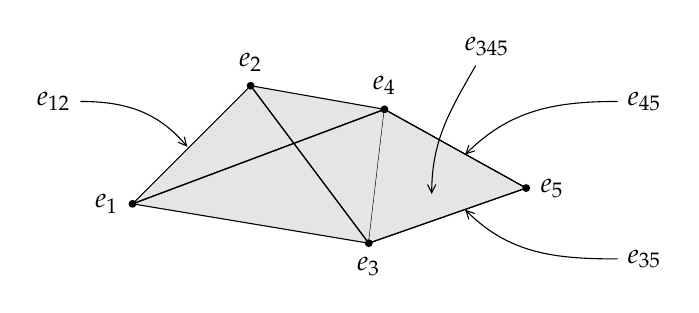
\begin{tikzpicture}[scale=1]
\draw[fill=gray!20] (0,0) -- (3,-0.5) -- (3.2,1.2)-- (0,0); 
\draw[fill=gray!20] (0,0) -- (1.5,1.5) -- (3.2,1.2)-- (0,0); \draw[] (1.5,1.5) -- (3,-0.5); 
\draw[fill=gray!20] (3,-0.5) -- (5,0.2) -- (3.2,1.2); 
\draw[color=black!100] (1.5,1.5) -- (3,-0.5) -- (5,0.2);
\draw[color=black!100] (0,0) -- (3.2,1.2) -- (5,0.2);

\node[circle, fill=black, inner sep=1pt, label=left:$e_1 $] (a) at (0,0) {}; 
\node[circle, fill=black, inner sep=1pt, label=above:$e_2 $] (b) at (1.5,1.5) {}; 
\node[circle, fill=black, inner sep=1pt, label=below:$e_3 $] (c) at (3,-0.5) {};
\node[circle, fill=black, inner sep=1pt, label=above:$e_4 $] (d) at (3.2,1.2) {}; 
\node[circle, fill=black, inner sep=1pt, label=right:$e_5 $] (e) at (5,0.2) {};

\node[] (x) at (-1,1.3) {$ e_{12} $}; \node[] (x') at (0.8,0.6) {};
\draw[-{Straight Barb[length=3pt,width=3pt]}] (x) edge[out=0, in=130] node[below] {} (x');

\node[] (y) at (6.5,1.3) {$ e_{45} $}; \node[] (y') at (4.1,0.5) {}; 
\draw[-{Straight Barb[length=3pt,width=3pt]}] (y) edge[out=180, in=45] node[below] {} (y');

\node[] (z) at (6.5,-0.7) {$e_{35} $}; \node[] (z') at (4.1,0.05) {};
\draw[-{Straight Barb[length=3pt,width=3pt]}] (z) edge[out=180, in=-45] node[below] {} (z');

\node[] (w) at (4.5,2) {$e_{345} $}; \node[] (w') at (3.8,0) {};
\draw[-{Straight Barb[length=3pt,width=3pt]}] (w) edge[out=-120, in=90] node[below] {} (w');
\end{tikzpicture} \end{center}
\par\end{center} Next suppose $R=\Bbbk[x,y,z,w]$ and let $\boldsymbol{m}_{\mathrm{K}}=x^{2},w^{2},zw,xy,y^{2}z^{2}$.
Then we obtain an $\boldsymbol{m}_{\mathrm{K}}$-labeled simplicial
complex $\Delta=(\Delta,\boldsymbol{m}_{\mathrm{K}})$ which is pictured
below: \begin{center}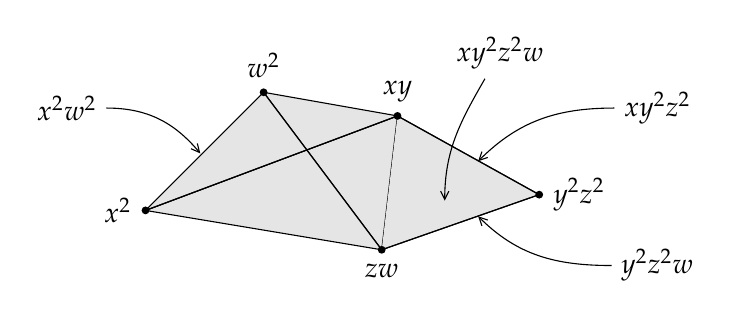
\begin{tikzpicture}[scale=1]

\draw[fill=gray!20] (0,0) -- (3,-0.5) -- (3.2,1.2)-- (0,0); 
\draw[fill=gray!20] (0,0) -- (1.5,1.5) -- (3.2,1.2)-- (0,0); 
\draw[] (1.5,1.5) -- (3,-0.5); \draw[fill=gray!20] (3,-0.5) -- (5,0.2) -- (3.2,1.2);
\draw[color=black!100] (1.5,1.5) -- (3,-0.5) -- (5,0.2);
\draw[color=black!100] (0,0) -- (3.2,1.2) -- (5,0.2);

\node[circle, fill=black, inner sep=1pt, label=left:$x^2 $] (a) at (0,0) {};
\node[circle, fill=black, inner sep=1pt, label=above:$w^2 $] (b) at (1.5,1.5) {};
\node[circle, fill=black, inner sep=1pt, label=below:$zw $] (c) at (3,-0.5) {};
\node[circle, fill=black, inner sep=1pt, label=above:$xy $] (d) at (3.2,1.2) {}; 
\node[circle, fill=black, inner sep=1pt, label=right:$y^2 z^2 $] (e) at (5,0.2) {};

\node[] (x) at (-1,1.3) {$ x^2 w^2 $}; \node[] (x') at (0.8,0.6) {};
\draw[-{Straight Barb[length=3pt,width=3pt]}] (x) edge[out=0, in=130] node[below] {} (x');

\node[] (y) at (6.5,1.3) {$ x y^2 z^2 $}; \node[] (y') at (4.1,0.5) {}; 
\draw[-{Straight Barb[length=3pt,width=3pt]}] (y) edge[out=180, in=45] node[below] {} (y');

\node[] (z) at (6.5,-0.7) {$ y^2 z^2 w $}; \node[] (z') at (4.1,0.05) {};
\draw[-{Straight Barb[length=3pt,width=3pt]}] (z) edge[out=180, in=-45] node[below] {} (z');

\node[] (w) at (4.5,2) {$ x y^2 z^2 w $}; \node[] (w') at (3.8,0) {}; 
\draw[-{Straight Barb[length=3pt,width=3pt]}] (w) edge[out=-120, in=90] node[below] {} (w');

\end{tikzpicture} \end{center} Let $F_{\mathrm{K}}$ be the $R$-complex induced by $\Delta$. Let's
write down the homogeneous components of $F_{\mathrm{K}}$ as a graded
$R$-module: we have
\begin{align*}
F_{\mathrm{K},0} & =R\\
F_{\mathrm{K},1} & =Re_{1}+Re_{2}+Re_{3}+Re_{4}+Re_{5}\\
F_{\mathrm{K},2} & =Re_{12}+Re_{13}+Re_{14}+Re_{23}+Re_{24}+Re_{34}+Re_{35}+Re_{45}\\
F_{\mathrm{K},3} & =Re_{123}+Re_{124}+Re_{134}+Re_{234}+Re_{345}\\
F_{\mathrm{K},4} & =Re_{1234}
\end{align*}
The differential $\mathrm{d}\colon F_{\mathrm{K}}\to F_{\mathrm{K}}$
behaves just like the usual simplicial boundary map except some monomials
can show up as coefficients. For instance,
\[
\mathrm{d}(e_{1234})=-ye_{123}+ze_{124}-we_{134}+xe_{234}.
\]
Now, we begin to construct a multiplication $(\mu,\star)$ on $F_{\mathrm{K}}$
as follows: first we want $\mu$ to respect the multigrading. Then
the multigrading and Leibniz law conditions that we impose on $\mu$
forces it to be defined uniquely on many homogeneous basis pairs $(e_{\sigma},e_{\tau})$.
For instance, we are forced to have
\begin{align}
e_{1}\star e_{5} & =yz^{2}e_{14}+xe_{45}\nonumber \\
e_{1}\star e_{2} & =e_{12}\nonumber \\
e_{2}\star e_{5} & =y^{2}ze_{23}+we_{35}\nonumber \\
e_{2}\star e_{45} & =-yze_{234}+we_{345}\label{eq:multkathan}\\
e_{1}\star e_{35} & =yze_{134}-xe_{345}\nonumber \\
e_{1}\star e_{23} & =e_{123}\nonumber \\
e_{2}\star e_{14} & =-e_{124}\nonumber 
\end{align}
At this point however, one can conclude that $F_{\mathrm{K}}$ is
not associative since
\begin{equation}
[e_{1},e_{5},e_{2}]:=(e_{1}\star e_{5})\star e_{2}-e_{1}\star(e_{5}\star e_{2})=-yz\mathrm{d}(e_{1234})\neq0.\label{eq:associatorsingular-1-1}
\end{equation}

One can work (\ref{eq:associatorsingular-1-1}) out by hand, however
one of the main results of our research is a method for calculating
associators like (\ref{eq:associatorsingular-1-1}) using tools from
the theory of Gr�bner bases. For instance, we used the following Singular
code below to calculate the associator $[e_{1},e_{5},e_{2}]$: \begin{center}
\begin{tabular}{|c|}
\hline 
\begin{lstlisting}
LIB "ncalg.lib"; 

intvec v= 1:3, 2:5, 3:5; 
ring A=(0,x,y,z,w),(e1,e2,e5,e12,e14,e23,e35,e45,e123,e124,e134,e234,e345),Wp(v);

matrix C[13][13]; matrix D[13][13]; int i; int j; 
for (i=1; i<=13; i++) {for (j=1; j<=13; j++) {C[i,j]=(-1)^(v[i]*v[j]);}} 
ncalgebra(C,D);

poly f(1)(5) = e1*e5-yz2*e14-x*e45;  
poly f(1)(2) = e1*e2-e12; 
poly f(2)(5) = e2*e5-y2z*e23-w*e35;  
poly f(2)(45) = e2*e45+yz*e234-w*e345;  
poly f(1)(35) = e1*e35-yz*e134+x*e345;  
poly f(1)(23) = e1*e23-e123;  
poly f(2)(14) = e2*e14+e124;
poly S(1)(5)(2) = f(1)(5)*e2+e1*f(2)(5);  

ideal I = f(2)(14),f(2)(45),f(1)(23),f(1)(35),f(2)(5),f(1)(5);
reduce(S(1)(5)(2),b); 

// [e1,e5,e2] = (y^2*z)*e123-(y*z^2)*e124+(y*z*w)*e134-(x*y*z)*e234
\end{lstlisting}
\tabularnewline
\hline 
\end{tabular}
\par\end{center} The multiplication isn't uniquely determined on all pairs $(e_{\sigma},e_{\tau})$,
for instance there are two possible ways in which we can define $\mu$
at the pair $(e_{5},e_{12})$. We choose to define $\mu$ at $(e_{5},e_{12})$
by
\[
e_{5}\star e_{12}=yz^{2}e_{124}+xyze_{234}+xwe_{345}.
\]
Finally, we would still like for $\mu$ to be as associative as possible
(even though we already know it's not associative at the triple $(e_{1},e_{5},e_{2})$).
In particular, we want $\mu$ to be associative on all triples of
the form $(e_{\sigma},e_{\sigma},e_{\tau})$. It turns out this can
be done. In fact, Singular tells us (e.g. by calculating a Gr�bner
basis of an ideal like the one in the code above) how we should define
$\mu$ at all other pairs $(e_{\sigma},e_{\tau})$ in order for this
to happen. \end{example}

\begin{example}\label{example2} Let $R=\Bbbk[x,y,z,w]$, let $\boldsymbol{m}_{\mathrm{A}}=x^{2},w^{2},zw,xy,yz$,
and let $F_{\mathrm{A}}$ be the minimal $R$-free resolution of $R\slash\boldsymbol{m}_{\mathrm{A}}$.
Then $F_{\mathrm{A}}$ can be realized as the $R$-complex induced
by the $\boldsymbol{m}_{\mathrm{A}}$-labeled cellular complex pictured
below: \begin{center}
\begin{tabular}{cccc}
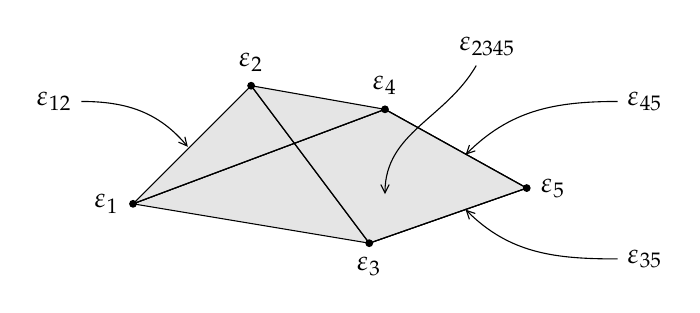
\begin{tikzpicture}[scale=1]

\draw[fill=gray!20] (0,0) -- (3,-0.5) -- (5,0.2) -- (3.2,1.2)-- (0,0); 
\draw[fill=gray!20] (0,0) -- (1.5,1.5) -- (3.2,1.2)-- (0,0); 
\draw[] (1.5,1.5) -- (3,-0.5); \draw[fill=gray!20] (3,-0.5) -- (5,0.2) -- (3.2,1.2);
\draw[color=black!100] (1.5,1.5) -- (3,-0.5) -- (5,0.2);
\draw[color=black!100] (0,0) -- (3.2,1.2) -- (5,0.2);

\node[circle, fill=black, inner sep=1pt, label=left:$\varepsilon _1 $] (a) at (0,0) {};
\node[circle, fill=black, inner sep=1pt, label=above:$\varepsilon _2 $] (b) at (1.5,1.5) {};
\node[circle, fill=black, inner sep=1pt, label=below:$\varepsilon _3 $] (c) at (3,-0.5) {};
\node[circle, fill=black, inner sep=1pt, label=above:$\varepsilon _4 $] (d) at (3.2,1.2) {}; 
\node[circle, fill=black, inner sep=1pt, label=right:$\varepsilon _5 $] (e) at (5,0.2) {};

\node[] (x) at (-1,1.3) {$ \varepsilon _{12} $}; \node[] (x') at (0.8,0.6) {};
\draw[-{Straight Barb[length=3pt,width=3pt]}] (x) edge[out=0, in=130] node[below] {} (x');

\node[] (y) at (6.5,1.3) {$ \varepsilon _{45} $}; \node[] (y') at (4.1,0.5) {}; 
\draw[-{Straight Barb[length=3pt,width=3pt]}] (y) edge[out=180, in=45] node[below] {} (y');

\node[] (z) at (6.5,-0.7) {$ \varepsilon _{35} $}; \node[] (z') at (4.1,0.05) {};
\draw[-{Straight Barb[length=3pt,width=3pt]}] (z) edge[out=180, in=-45] node[below] {} (z');

\node[] (w) at (4.5,2) {$ \varepsilon _{2345} $}; \node[] (w') at (3.2,0) {}; 
\draw[-{Straight Barb[length=3pt,width=3pt]}] (w) edge[out=-120, in=90] node[below] {} (w');

\end{tikzpicture} &  &  & 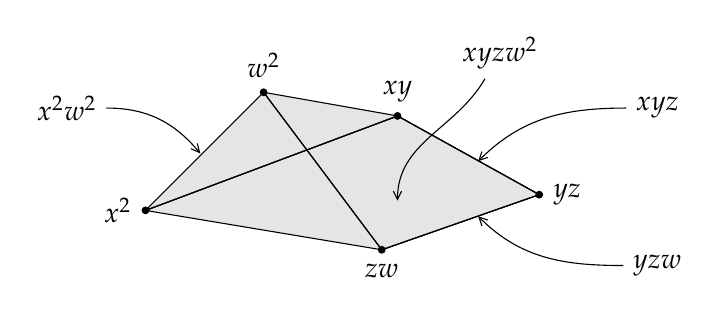
\begin{tikzpicture}[scale=1]

\draw[fill=gray!20] (0,0) -- (3,-0.5) -- (5,0.2) -- (3.2,1.2)-- (0,0); 
\draw[fill=gray!20] (0,0) -- (1.5,1.5) -- (3.2,1.2)-- (0,0); 
\draw[] (1.5,1.5) -- (3,-0.5); \draw[fill=gray!20] (3,-0.5) -- (5,0.2) -- (3.2,1.2);
\draw[color=black!100] (1.5,1.5) -- (3,-0.5) -- (5,0.2);
\draw[color=black!100] (0,0) -- (3.2,1.2) -- (5,0.2);

\node[circle, fill=black, inner sep=1pt, label=left:$x^2 $] (a) at (0,0) {};
\node[circle, fill=black, inner sep=1pt, label=above:$w^2 $] (b) at (1.5,1.5) {};
\node[circle, fill=black, inner sep=1pt, label=below:$zw $] (c) at (3,-0.5) {};
\node[circle, fill=black, inner sep=1pt, label=above:$xy $] (d) at (3.2,1.2) {}; 
\node[circle, fill=black, inner sep=1pt, label=right:$yz $] (e) at (5,0.2) {};

\node[] (x) at (-1,1.3) {$ x^2 w^2 $}; \node[] (x') at (0.8,0.6) {};
\draw[-{Straight Barb[length=3pt,width=3pt]}] (x) edge[out=0, in=130] node[below] {} (x');

\node[] (y) at (6.5,1.3) {$ x y z $}; \node[] (y') at (4.1,0.5) {}; 
\draw[-{Straight Barb[length=3pt,width=3pt]}] (y) edge[out=180, in=45] node[below] {} (y');

\node[] (z) at (6.5,-0.7) {$ y z w $}; \node[] (z') at (4.1,0.05) {};
\draw[-{Straight Barb[length=3pt,width=3pt]}] (z) edge[out=180, in=-45] node[below] {} (z');

\node[] (w) at (4.5,2) {$ x y z w^2 $}; \node[] (w') at (3.2,0) {}; 
\draw[-{Straight Barb[length=3pt,width=3pt]}] (w) edge[out=-120, in=90] node[below] {} (w');

\end{tikzpicture}\tabularnewline
\end{tabular}
\par\end{center} Let's write down the homogeneous components of $F_{\mathrm{A}}$
as a graded module: we have
\begin{align*}
F_{\mathrm{A},0} & =R\\
F_{\mathrm{A},1} & =R\varepsilon_{1}+R\varepsilon_{2}+R\varepsilon_{3}+R\varepsilon_{4}+R\varepsilon_{5}\\
F_{\mathrm{A},2} & =R\varepsilon_{12}+R\varepsilon_{13}+R\varepsilon_{14}+R\varepsilon_{23}+R\varepsilon_{24}+R\varepsilon_{35}+R\varepsilon_{45}\\
F_{\mathrm{A},3} & =R\varepsilon_{123}+R\varepsilon_{124}+R\varepsilon_{1345}+R\varepsilon_{2345}\\
F_{\mathrm{A},4} & =R\varepsilon_{12345}
\end{align*}
The differential $\mathrm{d}\colon F_{\mathrm{A}}\to F_{\mathrm{A}}$
on the non-simplicial faces is given below
\begin{align*}
\mathrm{d}(\varepsilon_{12345}) & =x\varepsilon_{2345}-z\varepsilon_{124}+w\varepsilon_{1345}-y\varepsilon_{123}\\
\mathrm{d}(\varepsilon_{1345}) & =x^{2}\varepsilon_{35}-xw\varepsilon_{45}-zw\varepsilon_{14}+y\varepsilon_{13}\\
\mathrm{d}(\varepsilon_{2345}) & =xw\varepsilon_{35}-w^{2}\varepsilon_{45}-z\varepsilon_{24}+xy\varepsilon_{23}.
\end{align*}
We obtain a multiplication on $F_{\mathrm{A}}$ from the one we constructed
on $F_{\mathrm{K}}$ as follows: first note that the canonical map
$R\slash\boldsymbol{m}_{\mathrm{K}}\to R\slash\boldsymbol{m}_{\mathrm{A}}$
induces a multigraded comparison map $\pi\colon F_{\mathrm{K}}\to F_{\mathrm{A}}$
defined by
\begin{align*}
\pi(e_{5}) & =yz\varepsilon_{5}\\
\pi(e_{35}) & =yz\varepsilon_{35}\\
\pi(e_{45}) & =yz\varepsilon_{45}\\
\pi(e_{34}) & =x\varepsilon_{35}-w\varepsilon_{45}\\
\pi(e_{345}) & =0\\
\pi(e_{234}) & =\varepsilon_{2345}\\
\pi(e_{134}) & =\varepsilon_{1345}\\
\pi(e_{1234}) & =\varepsilon_{12345}
\end{align*}
and $\pi(e_{\sigma})=\varepsilon_{\sigma}$ for the remaining homogeneous
basis elements. This map is locally invertible. Indeed, by base changing
to $R_{yz}$, we obtain quasiisomorphisms $F_{\mathrm{A},yz}\to0\leftarrow F_{\mathrm{K},yz}$.
In particular, there exists a comparison map $\iota\colon F_{\mathrm{A},yz}\to F_{\mathrm{K},yz}$
which splits comparison map $\pi\colon F_{\mathrm{K},yz}\to F_{\mathrm{A},yz}$.
By considering the multigrading as well as the Leibniz law, we see
that
\begin{align*}
\iota(\varepsilon_{5}) & =e_{5}/yz\\
\iota(\varepsilon_{35}) & =e_{35}/yz\\
\iota(\varepsilon_{45}) & =e_{45}/yz\\
\iota(\varepsilon_{2345}) & =-e_{234}+e_{345}/yz\\
\iota(\varepsilon_{1345}) & =e_{134}-e_{345}/yz\\
\iota(\varepsilon_{12345}) & =e_{1234}
\end{align*}
and $\iota(\varepsilon_{\sigma})=e_{\sigma}$ for the remaining homogeneous
basis elements. Then we defined a multiplication $\nu$ on $F$ using
the multiplication $\mu$ on $F_{\mathrm{K},yz}$ by setting
\begin{equation}
\varepsilon_{\sigma}\star_{\nu}\varepsilon_{\tau}=\pi(\iota(\varepsilon_{\sigma})\star_{\mu}\iota(\varepsilon_{\tau}))\label{eq:avmult}
\end{equation}
for all homogeneous basis elements $\varepsilon_{\sigma},\varepsilon_{\tau}$
of $F_{\mathrm{A},yz}$. It is straightforward to check that $\nu$
restricts to a multiplication on $F_{\mathrm{A}}$ (the coefficients
in (\ref{eq:avmult}) are all in $R$). Note that $\nu$ is not associative
since
\[
[\varepsilon_{1},\varepsilon_{5},\varepsilon_{2}]=-\mathrm{d}(\varepsilon_{1234})\neq0.
\]
\end{example}

\begin{example}\label{example3} Let $R=\Bbbk[x,y,z,w]$, let $\boldsymbol{m}_{\mathrm{M}}=x^{2},w^{2},zw,xy,y^{2}z,yz^{2}$,
and let $F_{\mathrm{M}}$ be the minimal $R$-free resolution of $R\slash\boldsymbol{m}_{\mathrm{M}}$.
Then $F_{\mathrm{M}}$ can be realized as the $R$-compex induced
by the $\boldsymbol{m}_{\mathrm{M}}$-labeled simplicial complex pictured
below: \begin{center}
\begin{tabular}{ccccc}
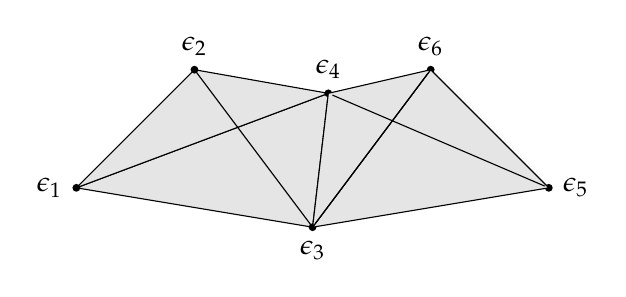
\begin{tikzpicture}[scale=1]
\draw[fill=gray!20] (0,0) -- (3,-0.5) -- (3.2,1.2)-- (0,0); 
\draw[fill=gray!20] (0,0) -- (1.5,1.5) -- (3.2,1.2)-- (0,0); 
\draw[] (1.5,1.5) -- (3,-0.5); 
 

\node[circle, fill=black, inner sep=1pt, label=left:$\epsilon _1 $] (e1) at (0,0) {}; 
\node[circle, fill=black, inner sep=1pt, label=above:$\epsilon _2 $] (e2) at (1.5,1.5) {}; 
\node[circle, fill=black, inner sep=1pt, label=below:$\epsilon _3 $] (e3) at (3,-0.5) {};
\node[circle, fill=black, inner sep=1pt, label=above:$\epsilon _4 $] (e4) at (3.2,1.2) {}; 
\node[circle, fill=black, inner sep=1pt, label=right:$\epsilon _5 $] (e5) at (6,0) {};
\node[circle, fill=black, inner sep=1pt, label=above:$\epsilon _6 $] (e6) at (4.5,1.5) {};

\draw[fill=gray!20] (3,-0.5) -- (6,0) -- (4.5,1.5) -- (3,-0.5);
\draw[fill=gray!20]  (3.2,1.2) -- (4.5,1.5) -- (3,-0.5) -- (3.2,1.2);

\draw[] (e4) -- (e5);
\draw[] (e3) -- (e6);

\end{tikzpicture} &  &  &  & 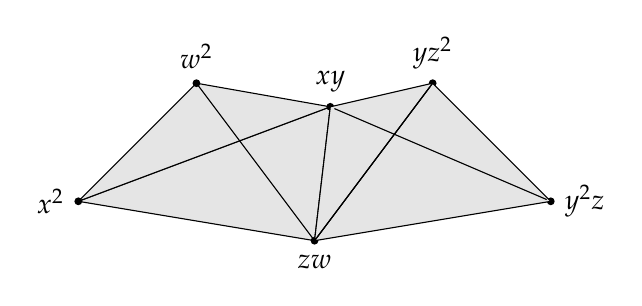
\begin{tikzpicture}[scale=1]
\draw[fill=gray!20] (0,0) -- (3,-0.5) -- (3.2,1.2)-- (0,0); 
\draw[fill=gray!20] (0,0) -- (1.5,1.5) -- (3.2,1.2)-- (0,0); 
\draw[] (1.5,1.5) -- (3,-0.5); 
 

\node[circle, fill=black, inner sep=1pt, label=left:$x^2 $] (e1) at (0,0) {}; 
\node[circle, fill=black, inner sep=1pt, label=above:$w^2 $] (e2) at (1.5,1.5) {}; 
\node[circle, fill=black, inner sep=1pt, label=below:$zw $] (e3) at (3,-0.5) {};
\node[circle, fill=black, inner sep=1pt, label=above:$xy $] (e4) at (3.2,1.2) {}; 
\node[circle, fill=black, inner sep=1pt, label=right:$y^2 z $] (e5) at (6,0) {};
\node[circle, fill=black, inner sep=1pt, label=above:$y z^2 $] (e6) at (4.5,1.5) {};

\draw[fill=gray!20] (3,-0.5) -- (6,0) -- (4.5,1.5) -- (3,-0.5);
\draw[fill=gray!20]  (3.2,1.2) -- (4.5,1.5) -- (3,-0.5) -- (3.2,1.2);

\draw[] (e4) -- (e5);
\draw[] (e3) -- (e6);

\end{tikzpicture}\tabularnewline
\end{tabular}
\par\end{center} Let's write down the homogeneous components of $F_{\mathrm{M}}$
as a graded $R$-module: we have
\begin{align*}
F_{\mathrm{M},0} & =R\\
F_{\mathrm{M},1} & =R\epsilon_{1}+R\epsilon_{2}+R\epsilon_{3}+R\epsilon_{4}+R\epsilon_{5}+R\epsilon_{6}\\
F_{\mathrm{M},2} & =R\epsilon_{12}+R\epsilon_{13}+R\epsilon_{14}+R\epsilon_{23}+R\epsilon_{24}+R\epsilon_{34}+R\epsilon_{35}+R\epsilon_{36}+R\epsilon_{45}+R\epsilon_{46}+R\epsilon_{56}\\
F_{\mathrm{M},3} & =R\epsilon_{123}+R\epsilon_{124}+R\epsilon_{134}+R\epsilon_{234}+R\epsilon_{345}+R\epsilon_{346}+R\epsilon_{356}+R\epsilon_{456}\\
F_{\mathrm{M},4} & =R\epsilon_{1234}+R\epsilon_{3456}.
\end{align*}
Note that the canonical map $R\slash\boldsymbol{m}_{\mathrm{K}}\to R\slash\boldsymbol{m}_{\mathrm{M}}$
induces a multigraded comparison map $\pi_{\lambda}\colon F_{\mathrm{K}}\to F_{\mathrm{M}}$
where $\lambda\in\Bbbk$ and where $\pi_{\lambda}$ is defined by
\begin{align*}
\pi_{\lambda}(e_{5}) & =\lambda z\epsilon_{5}+(1-\lambda)y\epsilon_{6}\\
\pi_{\lambda}(e_{35}) & =\lambda z\epsilon_{35}+(1-\lambda)y\epsilon_{36}\\
\pi_{\lambda}(e_{45}) & =\lambda z\epsilon_{45}+(1-\lambda)y\epsilon_{46}\\
\pi_{\lambda}(e_{345}) & =\lambda z\epsilon_{345}+(1-\lambda)y\epsilon_{346}
\end{align*}
and $\pi_{\lambda}(e_{\sigma})=\epsilon_{\sigma}$ for the remaining
homogeneous basis elements. We define a multiplication on $F_{\mathrm{M}}$
as follows: first we take the multiplications given in (\ref{eq:multkathan})
and we just replace $e_{1}$ with $\epsilon_{1}$, $e_{5}$ with $z\epsilon_{5}$,
$e_{14}$ with $\epsilon_{14}$, $e_{45}$ with $z\epsilon_{45}$,
and so on. For instance, we have
\begin{align*}
\epsilon_{1}\star\epsilon_{5} & =yz\epsilon_{14}+x\epsilon_{45} &  &  & \epsilon_{1}\star\epsilon_{6} & =z^{2}e_{14}+xe_{46}\\
\epsilon_{2}\star\epsilon_{5} & =y^{2}\epsilon_{23}+w\epsilon_{35} &  &  & \epsilon_{2}\star\epsilon_{6} & =yz\epsilon_{23}+w\epsilon_{36}\\
\epsilon_{2}\star\epsilon_{45} & =-y\epsilon_{234}+w\epsilon_{345} &  &  & \epsilon_{2}\star\epsilon_{46} & =-ze_{234}+w\epsilon_{345}\\
\epsilon_{1}\star\epsilon_{35} & =y\epsilon_{134}-x\epsilon_{345} &  &  & \epsilon_{1}\star\epsilon_{36} & =z\epsilon_{134}-x\epsilon_{346}.
\end{align*}
Note that $\mu$ is not associative since
\[
[\epsilon_{1},\epsilon_{5},\epsilon_{2}]=-y\mathrm{d}(\epsilon_{1234})\neq0\quad\text{and}\quad[\epsilon_{1},\epsilon_{6},\epsilon_{2}]=-z\mathrm{d}(\epsilon_{1234})\neq0.
\]

\end{example}

\begin{example}\label{example4} Let $R=\Bbbk[x,y,z,w]$, let $\boldsymbol{m}_{\mathrm{O}}=x^{2},w^{2},zw,xy,y^{2},z^{2}$,
and let $F_{\mathrm{O}}$ be the minimal $R$-free resolution of $R\slash\boldsymbol{m}_{\mathrm{O}}$.
Then $F_{\mathrm{O}}$ can be realized as the $R$-compex induced
by the $\boldsymbol{m}_{\mathrm{O}}$-labeled simplicial complex pictured
below:\begin{center}
\begin{tabular}{ccccc}
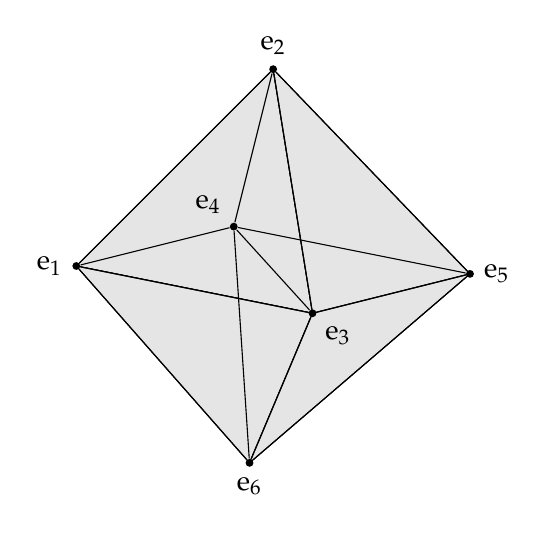
\begin{tikzpicture}

\draw[fill=gray!20] (-1,0) -- (2,-0.6) -- (1.5,2.5)-- (-1,0); 
\draw[fill=gray!20] (2,-0.6)  -- (1.5,2.5) -- (4,-0.1)-- (2,-0.6) ; 
\draw[fill=gray!20] (-1,0) -- (2,-0.6) -- (1.2,-2.5)-- (-1,0); 
\draw[fill=gray!20] (2,-0.6) -- (4,-0.1) -- (1.2,-2.5)-- (2,-0.6); 

\node[circle, fill=black, inner sep=1pt, label=left:$\mathrm{e}_1 $] (e1) at (-1,0) {}; 
\node[circle, fill=black, inner sep=1pt, label=above left :$\mathrm{e}_4 $] (e2) at (1,0.5) {}; 
\node[circle, fill=black, inner sep=1pt, label=below right:$\mathrm{e}_3 $] (e3) at (2,-0.6) {};
\node[circle, fill=black, inner sep=1pt, label=above:$\mathrm{e}_2 $] (e4) at (1.5,2.5) {}; 
\node[circle, fill=black, inner sep=1pt, label=right:$\mathrm{e}_5 $] (e5) at (4,-0.1) {};
\node[circle, fill=black, inner sep=1pt, label=below:$\mathrm{e}_6 $] (e6) at (1.2,-2.5) {};

\draw[] (e1) -- (e2);
\draw[] (e1) -- (e3);
\draw[] (e1) -- (e4);
\draw[] (e3) -- (e6);
\draw[] (e4) -- (e5);
\draw[] (e3) -- (e4);
\draw[] (e2) -- (e5);
\draw[] (e3) -- (e5);
\draw[] (e1) -- (e6);
\draw[] (e5) -- (e6);
\draw[] (e2) -- (e6);
\draw[] (e2) -- (e4);
\draw[] (e3) -- (e2);


\end{tikzpicture} &  &  &  & 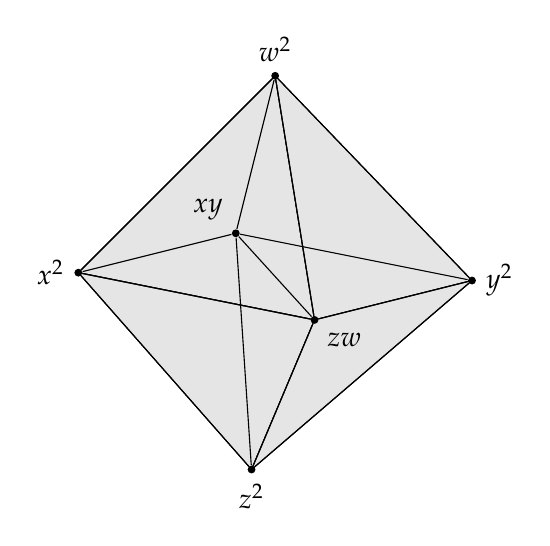
\begin{tikzpicture}

\draw[fill=gray!20] (-1,0) -- (2,-0.6) -- (1.5,2.5)-- (-1,0); 
\draw[fill=gray!20] (2,-0.6)  -- (1.5,2.5) -- (4,-0.1)-- (2,-0.6) ; 
\draw[fill=gray!20] (-1,0) -- (2,-0.6) -- (1.2,-2.5)-- (-1,0); 
\draw[fill=gray!20] (2,-0.6) -- (4,-0.1) -- (1.2,-2.5)-- (2,-0.6); 

\node[circle, fill=black, inner sep=1pt, label=left:$x^2 $] (e1) at (-1,0) {}; 
\node[circle, fill=black, inner sep=1pt, label=above left :$xy $] (e2) at (1,0.5) {}; 
\node[circle, fill=black, inner sep=1pt, label=below right:$zw $] (e3) at (2,-0.6) {};
\node[circle, fill=black, inner sep=1pt, label=above:$w^2 $] (e4) at (1.5,2.5) {}; 
\node[circle, fill=black, inner sep=1pt, label=right:$y^2 $] (e5) at (4,-0.1) {};
\node[circle, fill=black, inner sep=1pt, label=below:$z^2 $] (e6) at (1.2,-2.5) {};

\draw[] (e1) -- (e2);
\draw[] (e1) -- (e3);
\draw[] (e1) -- (e4);
\draw[] (e3) -- (e6);
\draw[] (e4) -- (e5);
\draw[] (e3) -- (e4);
\draw[] (e2) -- (e5);
\draw[] (e3) -- (e5);
\draw[] (e1) -- (e6);
\draw[] (e5) -- (e6);
\draw[] (e2) -- (e6);
\draw[] (e2) -- (e4);
\draw[] (e3) -- (e2);


\end{tikzpicture}\tabularnewline
\end{tabular}
\par\end{center} One can show that there is a multigraded multiplication that one
can define on $F_{\mathrm{O}}$ which turns out to be associative.
We define it below on some of the homogeneous basis elements:
\begin{align*}
\mathrm{e}_{1}\star\mathrm{e}_{5} & =y\mathrm{e}_{14}+x\mathrm{e}_{45}\\
\mathrm{e}_{2}\star\mathrm{e}_{6} & =z\mathrm{e}_{23}+w\mathrm{e}_{35}\\
\mathrm{e}_{1}\star\mathrm{e}_{25} & =y\mathrm{e}_{124}-x\mathrm{e}_{245}\\
\mathrm{e}_{1}\star\mathrm{e}_{35} & =y\mathrm{e}_{134}-x\mathrm{e}_{345}\\
\mathrm{e}_{1}\star\mathrm{e}_{56} & =y\mathrm{e}_{146}+x\mathrm{e}_{456}\\
\mathrm{e}_{2}\star\mathrm{e}_{16} & =-z\mathrm{e}_{123}-w\mathrm{e}_{136}\\
\mathrm{e}_{2}\star\mathrm{e}_{46} & =-z\mathrm{e}_{234}+w\mathrm{e}_{346}\\
\mathrm{e}_{2}\star\mathrm{e}_{56} & =-z\mathrm{e}_{235}+w\mathrm{e}_{356}\\
\mathrm{e}_{2}\star\mathrm{e}_{146} & =\mathrm{e}_{1234}+\mathrm{e}_{1346}\\
\mathrm{e}_{2}\star\mathrm{e}_{456} & =\mathrm{e}_{2345}+\mathrm{e}_{3456}\\
\mathrm{e}_{1}\star\mathrm{e}_{235} & =\mathrm{e}_{1234}+\mathrm{e}_{2345}\\
\mathrm{e}_{1}\star\mathrm{e}_{356} & =\mathrm{e}_{1346}+\mathrm{e}_{3456}.
\end{align*}

\end{example} 

\subsubsection{Multigraded Multiplications coming from the Taylor Algebra}

In this subsubsection, we want to explain how all of the multigraded
multiplications that we've considered in the examples above come from
a Taylor multiplication in the following sense: let $R=\Bbbk[x_{1},\dots,x_{d}]$,
let $I$ be a monomial ideal in $R$, let $F$ be the minimal $R$-free
resolution of $R\slash I$, and let $T$ be the Taylor algebra resolution
of $R\slash I$. The Taylor multiplication is denoted $\nu_{T}$.
Let $\nu$ be a possibly different multiplication on $T$. We write
$T_{\nu}$ to be the MDG $R$-algebra whose underlying $R$-complex
is the same as the underlying complex of $T$ but whose multiplication
is $\nu$. Since $F$ is the minimal $R$-free resolution of $R\slash I$
and since $T$ is an $R$-free resolution of $R\slash I$, there exists
multigraded chain maps $\iota\colon F\to T$ and $\pi\colon T\to F$
which lift the identity map $R\slash I\to R\slash I$ such that $\iota\colon F\to T$
is injective and is split by $\pi\colon T\to F$, meaning $\pi\iota=1$.
By identifying $F$ with $\iota(F)$ if necessary, we may assume that
$\iota\colon F\subseteq T$ is inclusion and that $\pi\colon T\to F$
is a \textbf{projection}, meaning $\pi\colon T\to F$ is a surjective
chain map which satisfies $\pi^{2}=\pi$, or alternatively, $\pi\colon T\to T$
is a chain map with $\mathrm{im}\,\pi=F$. In what follows, we fix
$\iota\colon F\subseteq T$ once and for all and we denote by $\mathcal{P}(T,F)$
to be the set of all projections $\pi\colon T\to F$. For each $\mu\in\mathrm{Mult}(F)$,
we denote by $\mathrm{Mult}(T\slash\mu)$ to be the set of all multiplications
on $T$ which extends $\mu$:
\[
\mathrm{Mult}(T\slash\mu)=\{\nu\in\mathrm{Mult}(T)\mid\nu|_{F^{\otimes2}}=\nu\iota^{\otimes2}=\mu\}.
\]

Observe that if $\pi\in\mathcal{P}(T,F)$ and $\nu\in\mathrm{Mult}(T\slash\mu)$,
then $\pi\nu\in\mathrm{Mult}(T\slash\mu)$. Indeed, $\pi\nu$ is clearly
a multiplication on $T$. Furthermore, since $\pi$ is a projective
and since $\mu$ lands in $F$, we have $\pi\mu=\mu$. Therefore
\[
\pi\nu\iota^{\otimes2}=\pi\mu=\mu,
\]
so $\pi\nu$ restricts to $\mu$ as well. Next, observe that if $\pi\in\mathcal{P}(T,F)$
and $\mu\in\mathrm{Mult}(F)$, then $\widehat{\mu}_{\pi}:=\mu\pi^{\otimes2}\in\mathrm{Mult}(T\slash\mu)$.
We call $\widehat{\mu}=\widehat{\mu}_{\pi}$ the \textbf{trivial extension
}of $\mu$ with respect to $\pi$ for the following reasons: first
note that for each $\nu\in\mathrm{Mult}(T\slash\mu)$, the inclusion
map $\iota\colon F_{\mu}\subseteq T_{\nu}$ is multiplicative since
$\nu\iota^{\otimes2}=\mu=\iota\mu$, however $\pi\colon T_{\nu}\to F_{\mu}$
need not be multiplicative in general. In the case of the trivial
extension $\widehat{\mu}$ however, $\pi\colon T_{\widehat{\mu}}\to F_{\mu}$
is multiplicative since
\[
\pi\widehat{\mu}=\pi\mu\pi^{\otimes2}=\mu\pi^{\otimes2}.
\]
Next, note that since $\pi\colon T\to F$ splits the inclusion $\iota\colon F\subseteq T$,
we obtain isomorphism $\theta_{\pi}\colon T\simeq F\oplus H$ of $R$-complexes,
where $H=\ker\pi$ is a trivial $R$-complex with $H_{0}=0=H_{1}$,
and where $\theta_{\pi}=(\pi,1-\pi)$. There's an obvious multiplication
that we can give $F\oplus H$, namely $\mu\oplus0$, where $0\colon H\otimes H\to H$
is the zero map. Equip $F\oplus H$ with this multiplication. We claim
that $\theta_{\pi}\colon T_{\widehat{\mu}}\to F\oplus H$ is multiplicative,
and hence an isomorphism of MDG $R$-algebras. Indeed, we have
\begin{align*}
\theta_{\pi}\widehat{\mu} & =(\pi\widehat{\mu},(1-\pi)\widehat{\mu})\\
 & =(\pi\widehat{\mu},\widehat{\mu}-\pi\widehat{\mu})\\
 & =(\widehat{\mu},\widehat{\mu}-\widehat{\mu})\\
 & =(\widehat{\mu},0)\\
 & =(\mu\pi^{\otimes2},0)\\
 & =(\mu\oplus0)(\pi^{\otimes2},1-\pi^{\otimes2})\\
 & =(\mu\oplus0)\theta_{\pi}^{\otimes2}.
\end{align*}
In particular, every $b\in T$ can expressed in the form $b=a+c$
for unique $a\in F$ and unique $c\in H$. If $b_{1},b_{2}\in T$
have the unique expressions $b_{1}=a_{1}+c_{1}$ and $b_{2}=a_{2}+c_{2}$,
then we have $b_{1}\star_{\nu}b_{2}=a_{1}\star_{\mu}a_{2}.$

\begin{example}\label{example} The multiplication $\mu$ in Example~(\ref{example1})
is given by $\mu=\pi\nu_{T}\iota^{\otimes2}$ where $T$ is the taylor
algebra resolution of $R\slash\boldsymbol{m}_{\mathrm{M}}$ and where
$\pi\colon T\to F$ is defined by
\begin{align*}
\pi(e_{15}) & =yz^{2}e_{14}+xe_{45}\\
\pi(e_{25}) & =y^{2}ze_{23}+we_{35}\\
\pi(e_{245}) & =-yze_{234}+we_{35}\\
\pi(e_{235}) & =0\\
\pi(e_{2345}) & =0\\
 & \vdots
\end{align*}
and so on. \end{example}

\subsection{MDG Modules}

We now want to define MDG $A$-modules where $A$ is an MDG $R$-algebra.

\begin{defn}\label{defn} Let $X$ be an $R$-complex equipped with
chain maps $\mu_{A,X}\colon A\otimes_{R}X\to X$ and $\mu_{X,A}\colon X\otimes_{R}A\to X$,
denoted $a\otimes x\mapsto ax$ and $x\otimes a\mapsto xa$ respectively.
\begin{enumerate}
\item We say $X$ is \textbf{unital }if $1x=x=x1$ for all $x\in X$.
\item We say $X$ is \textbf{graded-commutative} if $ax=(-1)^{|a||x|}xa$
for all $a\in A$ homogeneous and $x\in X$ homogeneous. In this case,
$\mu_{X,A}$ is completely determined by $\mu_{A,X}$, and thus we
completely forget about it and write $\mu_{X}=\mu_{A,X}$.
\item We say $X$ is \textbf{associative }if $a_{1}(a_{2}x)=(a_{1}a_{2})x$
for all $a_{1},a_{2}\in A$ and $x\in X$.
\end{enumerate}
We say $X$ is an \textbf{MDG $A$-module }if it is graded-commutative,
unital, and the graded $R$-linear map
\[
\overline{\mu}_{X}\colon\mathrm{H}(A)\otimes_{R}\mathrm{H}(X)\to\mathrm{H}(X)
\]
induced by $\mu_{X}$ gives $\mathrm{H}(X)$ the structure of an associative
graded-commutative $\mathrm{H}(A)$-module. We call $\mu_{X}$ the
$A$\textbf{-scalar multiplication }of $X$. If $X$ is also associative,
then we say $X$ is a\textbf{ DG $A$-module}. A map $\varphi\colon X\to Y$
between MDG $A$-modules $X$ and $Y$ is called an \textbf{MDG $A$-module
homomorphism }if it is a chain map which is also \textbf{multiplicative},
meaning $\varphi(ax)=a\varphi(x)$ for all $a\in A$ and $x\in X$.
We obtain a category, denoted $\mathbf{Mod}_{A}^{\star}$, whose objects
are MDG $A$-modules and whose morphisms are MDG $A$-module homomorphisms.
\end{defn}

\begin{example}\label{example} Let $A$ and $B$ be MDG $R$-algebras
and let $\varphi\colon A\to B$ be a chain map such that $\varphi(1)=1$.
Then we give $B$ the structure of an MDG $A$-module by defining
an $A$-scalar multiplication on $B$ via
\[
a\cdot b=\varphi(a)b
\]
for all $a\in A$ and $b\in B$. Note that we need $\varphi(1)=1$
in order for $B$ to be unital as an MDG $A$-module. Also note that
$\varphi$ is an MDG $A$-module homomorphism if and only if it is
an algebra homomorphism. Indeed, it is an $A$-module homomorphism
if and only if for all $a_{1},a_{2}\in A$ we have
\[
\varphi(a_{1}a_{2})=a_{1}\cdot\varphi(a_{2})=\varphi(a_{1})\varphi(a_{2}),
\]
which is equivalent to saying $\varphi$ is an algebra homomorphism
(since we already have $\varphi(1)=1$). \end{example}

\subsubsection{The Category of All MDG $A$-Modules}

Let $A$ be an MDG $R$-algebra. The category of all MDG $A$-modules
forms an abelian category which is enriched over the category of all
$R$-modules. Indeed, if $X$ and $Y$ are MDG $A$-modules, then
the set of all MDG $A$-module homomorphims from $X$ to $Y$, denoted
$\mathrm{Hom}_{A}(X,Y)$, has the structure of an $R$-module, and
moreover, the usual composition operation
\[
\circ\colon\mathrm{Hom}_{A}(Y,Z)\times\mathrm{Hom}_{A}(X,Y)\to\mathrm{Hom}_{A}(X,Z),
\]
denoted $(g,f)\mapsto g\circ f=fg$, is $R$-bilinear. We also have
a zero object, binary biproducts, as well as kernels and cokernels.
For instance, if $\varphi\colon X\to Y$ is an MDG $A$-module homomorphism,
then the kernel of $\varphi$, denoted $\ker\varphi$, is defined
in the usual way as
\[
\ker\varphi=\{x\in X\mid\varphi(x)=0\}
\]
together with the canonical inclusion map $\iota\colon\ker\varphi\to X$.
The differential and $A$-scalar multiplication of $\ker\varphi$
are simply the ones obtained from $X$ via restriction to $\ker\varphi$.
Similarly the cokernel of $\varphi$ is defined in the usual way as
well. Thus the category of all MDG $A$-modules shares many of the
same properties as the category of all DG $B$-modules where $B$
is a DG $R$-algebra. Thus, the language we use in the category of
MDG $A$-modules is often similar to the language used in the category
of all DG $B$-modules. For instance, if $X$ and $Y$ are two MDG
$A$-modules such that $X\subseteq Y$, then we say $X$ is an \textbf{MDG
$A$-submodule }of $Y$ if the inclusion map $\iota\colon X\to Y$
is an MDG $A$-module homomorphism. In particular, this means that
both the differential and $A$-scalar multiplication of $Y$ restricts
to a differential and $A$-scalar multiplication on $X$. Similarly,
the MDG $A$-submodules $\mathfrak{a}$ of $A$ are often called \textbf{MDG
ideals }of $A$ or \textbf{MDG} $A$\textbf{-ideals}. An MDG $A$-ideal
$\mathfrak{p}$ is called a \textbf{prime ideal }if it satisfies the
following property: if $a_{1},a_{2}\in A$ such that $a_{1}a_{2}\in\mathfrak{p}$
and $a_{2}\notin\mathfrak{p}$, then $a_{1}\in\mathfrak{p}$. 

~~~Having said all of this, there are some notable differences
between the category of all DG $B$-modules and the category of all
MDG $A$-modules. In particular, one must be careful when defining
localization, tensor, and hom in the latter. In particular, if $X$
and $Y$ are MDG $A$-modules, then one can define the tensor complex
$X\otimes_{A}Y$ as well as the hom complex $\mathrm{Hom}_{A}^{\star}(X,Y)$
in the usual way. Then tensor complex $X\otimes_{A}Y$ turns out to
be an MDG $A$-module with the obvious $A$-scalar multiplication,
however it need not be true that $A\otimes_{A}X\simeq X$. On the
other hand, it may not be possible to give the hom complex $\mathrm{Hom}_{A}^{\star}(X,Y)$
the structure of an MDG $A$-module by defining $A$-scalar multiplication
in the obvious way. Finally, if $S\subseteq A$ is a multiplicatively
closed set, then one can make sense of the localization $X_{S}$,
but only in the case where $S$ satisfies some extra conditions. We
include more details on this in the appendix.

\begin{rem}\label{rem} Let $A$ be an MDG algebra and let \begin{equation}\label{equationjklfsddd}\begin{tikzcd} 0 \arrow[r] &  X \arrow[r, "\varphi  "] &  Y \arrow[r, "\psi " ] &  Z \arrow[r] & 0 \end{tikzcd}\end{equation}be
a short exact sequence of MDG $A$-modules. If we just view (\ref{equationjklfsddd})
as a short exact sequence of chain complexes, then we know that we
get an induced long exact sequence of abelian groups: \begin{equation}\label{connedctingjkd}\begin{tikzcd}[row sep=40]  \cdots \arrow[r] & \mathrm{H}_{i+1} ( Y ) \arrow[r, "\psi _{i+1} "] \arrow[d, phantom, ""{coordinate, name=Z'}] & \mathrm{H}_{i+1} (Z) \arrow[dll, "\partial _{i+1}  ", swap, rounded corners, to path={ -- ([xshift=2ex]\tikztostart.east) |- (Z') [near end]\tikztonodes -| ([xshift=-2ex]\tikztotarget.west) -- (\tikztotarget)}]\\   \mathrm{H}_{i} (X) \arrow[r, "\varphi _i "] & \mathrm{H}_{i}(Y) \arrow[r, "\psi _i "] \arrow[d, phantom, ""{coordinate, name=Z'}] & \mathrm{H}_{i} (Z) \arrow[dll, "\partial _i  ", swap, rounded corners, to path={ -- ([xshift=2ex]\tikztostart.east) |- (Z') [near end]\tikztonodes -| ([xshift=-2ex]\tikztotarget.west) -- (\tikztotarget)}] \\  \mathrm{H}_{i-1} (X) \arrow[r, "\varphi _{i-1} "]  & \mathrm{H}_{i-1}( Y ) \arrow[r] & \cdots \end{tikzcd}\end{equation}where
the connecting map $\partial\colon\mathrm{H}(Z)\to\mathrm{H}(X)$
is a graded $\mathrm{H}_{0}(A)$-module homorphism of degree $-1$
which is defined as follows: let $\overline{z}\in\mathrm{H}(Z)$ where
$z\in Z$ is homogeneous and $\mathrm{d}z=0$. Choose $y\in Y$ such
that $\psi y=z$. Then there is a unique $x\in X$ such that $\varphi x=\mathrm{d}y$.
We set $\partial\overline{z}=\overline{x}$ and verify that this is
a well-defined map (i.e. doesn't depend on any of the choices we made).
However we get more when we obtain a little more when we view (\ref{equationjklfsddd})
as a short exact sequence of MDG $A$-modules. Indeed, $\partial$
is not just an $\mathrm{H}_{0}(A)$-linear: it is $\mathrm{H}(A)$-linear!
Thus we obtain a sequence of graded $\mathrm{H}(A)$-modules: \begin{center}\begin{tikzcd}  \mathrm{H}(X) \arrow[r, "\varphi "] & \mathrm{H}(Y) \arrow[r, "\psi " ] & \mathrm{H}(Z) \arrow[r, " \partial " ]  & \Sigma \mathrm{H}(X)  \arrow[r, "\varphi " ] & \Sigma \mathrm{H}(Y) \end{tikzcd}\end{center}
which is exact at $\mathrm{H}(Y)$, $\mathrm{H}(Z)$, and $\Sigma\mathrm{H}(X)$.
\end{rem}

\section{Associators and Multiplicators}

In order to get a better understanding as to how far away MDG objects
are from being DG objects, we need to discuss associators and multiplicators.
Associators will help us measure how far away an MDG $A$-module $X$
is from being associative, whereas multiplicators will help up measure
how far away a chain map $\varphi\colon X\to Y$ is from being multiplicative.

\subsection{Associators}

We begin by defining associators. Throughout this subsection, let
$A$ be an MDG $R$-algebra and let $X$ be an MDG $A$-module. 

\begin{defn}\label{defnmulthompermcomp} The \textbf{associator }of
$X$ is the chain map, denoted $[\cdot]_{X}$ (or more simply by $[\cdot]$
if $X$ is understood from context), from $A\otimes_{R}A\otimes_{R}X$
to $X$ defined by
\[
[\cdot]:=\mu(\mu\otimes1-1\otimes\mu).
\]
Note that we use $\mu$ to denote both the multiplication $\mu_{A}$
on $A$ and the $A$-scalar multiplication $\mu_{X}$ on $X$ where
context makes clear which multiplication $\mu$ refers to. We denote
by $[\cdot,\cdot,\cdot]\colon A\times A\times X\to X$ to be the unique
$R$-trilinear map which corresponds to $[\cdot]$ via the universal
mapping property of tensor products. Thus we have
\[
[a_{1}\otimes a_{2}\otimes x]=(a_{1}a_{2})x-a_{1}(a_{2}x)=[a_{1},a_{2},x]
\]
for all $a_{1},a_{2}\in A$ and $x\in X$. \end{defn}

\subsubsection{Associator Identities}

In order to familiarize ourselves with the associator we collect together
some useful identities that the associator satisfies in this subsubsection:
\begin{itemize}
\item For all $a_{1},a_{2}\in A$ homogeneous and $x\in X$ we have the
Leibniz law
\begin{equation}
\mathrm{d}[a_{1},a_{2},x]=[\mathrm{d}a_{1},a_{2},x]+(-1)^{|a_{1}|}[a_{1},\mathrm{d}a_{2},x]+(-1)^{|a_{1}|+|a_{2}|}[a_{1},a_{2},\mathrm{d}x].\label{eq:leibnizlaw7}
\end{equation}
\item For all $a_{1},a_{2}\in A$ homogeneous and $x\in X$ homogeneous
we have
\begin{equation}
[a_{1},a_{2},x]=-(-1)^{|a_{1}||a_{2}|+|a_{1}||x|+|a_{2}||x|}[x,a_{2},a_{1}].\label{eq:identity3}
\end{equation}
\item For all $a_{1},a_{2}\in A$ homogeneous and $x\in X$ homogeneous
we have
\begin{equation}
[a_{1},a_{2},x]=-(-1)^{|a_{1}||x|+|a_{2}||x|}[x,a_{1},a_{2}]-(-1)^{|a_{1}||a_{2}|+|a_{1}||x|}[a_{2},x,a_{1}]\label{eq:identity2}
\end{equation}
\item For all $a_{1},a_{2}\in A$ homogeneous and $x\in X$ homogeneous
we have
\begin{equation}
[a_{1},a_{2},x]=(-1)^{|a_{1}||a_{2}|}[a_{2},a_{1},x]+(-1)^{|a_{2}||x|}[a_{1},x,a_{2}]\label{eq:identity4-1}
\end{equation}
\item For all $a_{1},a_{2},a_{3}\in A$ and $x\in X$ we have
\begin{equation}
a_{1}[a_{2},a_{3},x]=[a_{1}a_{2},a_{3},x]-[a_{1},a_{2}a_{3},x]+[a_{1},a_{2},a_{3}x]-[a_{1},a_{2},a_{3}]x\label{eq:identity1}
\end{equation}
\end{itemize}
The way the signs in (\ref{eq:identity3}) show up can be interpreted
as follows: in order to go from $[a_{1},a_{2},x]$ to $[x,a_{2},a_{1}]$,
we have to first swap $a_{1}$ with $a_{2}$ (this is where the $(-1)^{|a_{1}|a_{2}|}$
comes from), then swap $a_{1}$ with $x$ (this is where the $(-1)^{|a_{1}||x|}$
comes from), and then finally swap $a_{2}$ with $x$ (this is where
the $(-1)^{|a_{2}||x|}$ comes from). We then obtain one extra minus
sign by swapping terms in the associator at the final step:
\begin{align*}
[a_{1},a_{2},x] & =(a_{1}a_{2})x-a_{1}(a_{2}x)\\
 & =(-1)^{|a_{1}|a_{2}|}(a_{2}a_{1})x-(-1)^{|a_{2}|||x|}a_{1}(xa_{2})\\
 & =(-1)^{|a_{1}||a_{2}|+|a_{2}||x|+|a_{1}||x|}x(a_{2}a_{1})-(-1)^{|a_{2}||x|+|a_{1}||x|+|a_{1}||a_{2}|}(xa_{2})a_{1}\\
 & =(-1)^{|a_{1}||a_{2}|+|a_{1}||x|+|a_{2}||x|}(x(a_{2}a_{1})-(xa_{2})a_{1})\\
 & =-(-1)^{|a_{1}||a_{2}|+|a_{1}||x|+|a_{2}||x|}[x,a_{2},a_{1}].
\end{align*}
A similar interpretation is also given to (\ref{eq:identity2}) and
(\ref{eq:identity4-1}). For instance, in order to get from $[a_{1},a_{2},x]$
to $[x,a_{1},a_{2}]$, we have to swap $x$ with $a_{2}$ and then
swap $x$ with $a_{1}$ (this is where the $(-1)^{|a_{1}||x|+|a_{2}||x|}$
comes from). We do add an extra minus sign in (\ref{eq:identity4-1})
however since we never swap terms in the associator:
\begin{align*}
(-1)^{|a_{1}||a_{2}|}[a_{2},a_{1},x]+(-1)^{|a_{2}||x|}[a_{1},x,a_{2}] & =(a_{1}a_{2})x-(-1)^{|a_{1}||a_{2}|}a_{2}(a_{1}x)+(-1)^{|a_{2}||x|}(a_{1}x)a_{2}-a_{1}(a_{2}x)\\
 & =(a_{1}a_{2})x-(-1)^{|a_{1}||a_{2}|}a_{2}(a_{1}x)+(-1)^{|a_{1}|a_{2}|}a_{2}(a_{1}x)-a_{1}(a_{2}x)\\
 & =(a_{1}a_{2})x-a_{1}(a_{2}x)\\
 & =[a_{1},a_{2},x].
\end{align*}


\subsubsection{Alternative MDG Modules}

If $X$ is not associative, then one is often interested in knowing
whether or not $X$ satisfies the following weaker property:

\begin{defn}\label{defn} We say $X$ is \textbf{alternative }if $[a,a,x]=0$
for all $a\in A$ and $x\in X$. \end{defn}

~~~In other words, $X$ is alternative if for each $a\in A$ and
$x\in X$, we have $a^{2}x=a(ax).$ The reason behind the name ``alternative''
comes from the fact that in the case where $X=A$, then $A$ is alternative
if and only if the associator $[\cdot,\cdot,\cdot]$ is alternating.

\begin{prop}\label{propalternative} Let $a\in A$ and $x\in X$ be
homogeneous.
\begin{enumerate}
\item We have $[a,a,x]=0$ if and only if $[x,a,a]=0$.
\item If $[a,a,x]=0$, then $[a,x,a]=0$. The converse holds if $|a|$ is
odd and $\mathrm{char}\,R\ne2$.
\item If $|a|$ is even, we have $[a,x,a]=0$, and if $|a|$ is odd, we
have $[a,x,a]=(-1)^{|x|}2[a,a,x]$. In particular, if $\mathrm{char}\,R=2$,
we always have $[a,x,a]=0$. 
\end{enumerate}
\end{prop}

\begin{proof} From identities (\ref{eq:identity3}) and (\ref{eq:identity4-1})
we obtain
\begin{align*}
[a,a,x] & =-(-1)^{|a|}[x,a,a]\\{}
[a,x,a] & =(-1)^{|x||a|}(1-(-1)^{|a|})[a,a,x].
\end{align*}
In particular, we see that
\begin{equation}
[a,x,a]=\begin{cases}
=(-1)^{|x|}2[a,a,x]=-(-1)^{|x|}2a(ax) & \text{if }a\text{ is odd}\\
0 & \text{if }a\text{ is even}
\end{cases}\label{eq:relationshipcommut-1}
\end{equation}
Similarly we have
\begin{equation}
[a,a,x]=\begin{cases}
(-1)^{|x|}\frac{1}{2}[a,x,a] & \text{if }a\text{ is odd}\text{ and }\mathrm{char}\,R\neq2\\
(-1)^{|a|}[x,a,a] & \text{if }a\text{ is even}
\end{cases}\label{eq:relationshipcommut-1-1}
\end{equation}
\end{proof}

\begin{rem}\label{rem} Suppose $F$ is an MDG $R$-algebra whose
underlying graded $R$-module is finite and free with $e_{1},\dots,e_{n}$
being a homogeneous basis. In order to show $F$ is alternative, it
is \emph{not }enough to check $[e_{i},e_{i},e_{j}]=0$ for all $e_{i},e_{j}$
in the homogeneous basis. Indeed, even in this case, observe that
if $e_{i}$ and $e_{j}$ are odd, then
\begin{align*}
[e_{i}+e_{j},e_{i}+e_{j},e_{k}] & =[e_{i},e_{i},e_{k}]+[e_{i},e_{j},e_{k}]+[e_{j},e_{i},e_{k}]+[e_{j},e_{j},e_{k}]\\
 & =[e_{i},e_{j},e_{k}]+[e_{j},e_{i},e_{k}]\\
 & =[e_{i},e_{j},e_{k}]-[e_{j},e_{i},e_{k}]+(-1)^{|e_{k}|}[e_{j},e_{k},e_{i}]\\
 & =(-1)^{|e_{k}|}[e_{j},e_{k},e_{i}].
\end{align*}
Thus in order for $F$ to be alternative, we certainly need $[a_{1},a_{2},a_{3}]=0$
for all $a_{1},a_{2},a_{3}\in F$ whenever both $|a_{1}|$ and $|a_{3}|$
are odd. For instance, consider the MDG $R$-algebra $F_{\mathrm{K}}$
given in Example~(\ref{example1}). Then we have $[e_{\sigma},e_{\sigma},e_{\tau}]=0$
for all $\sigma,\tau\in\Delta$, however $F$ is not alternative since
$[e_{1},e_{5},e_{2}]\neq0$. \end{rem}

\subsubsection{The Maximal Associative Quotient}

\begin{defn}\label{defn} The \textbf{associator $R$-subcomplex }of
$X$, denoted $[X]$, is the $R$-subcomplex of $X$ given by the
image of the associator of $X$. Thus the underlying graded $R$-module
of $[X]$ is
\[
[X]=\mathrm{span}_{R}\{[a_{1},a_{2},x]\mid a_{1},a_{2}\in A\text{ and }x\in X\},
\]
and the differential of $[X]$ is simply the restriction of the differential
of $X$ to $[X]$. The \textbf{associator $A$-submodule }of $X$,
denoted $\langle X\rangle$, is defined to be the smallest $A$-submodule
of $X$ which contains $[X]$. The underlying graded $R$-module of
$\langle X\rangle$ also has a simple description. Indeed, observe
that
\begin{equation}
a_{1}(a_{2}[a_{3},a_{4},x])=(a_{1}a_{2})[a_{3},a_{4},x]-[a_{1},a_{2},[a_{3},a_{4},x]]\label{eq:jklfdsm-1}
\end{equation}
for all $a_{1},a_{2},a_{3},a_{4}\in A$ and $x\in X$. Using identities
like (\ref{eq:jklfdsm-1}) together with graded-commutativity, one
can show that the underlying graded $R$-module of $\langle X\rangle$
is given by 
\[
\langle X\rangle=\mathrm{span}_{R}\{a_{1}[a_{2},a_{3},x]\mid a_{1},a_{2},a_{3}\in A\text{ and }x\in X\}
\]

The quotient $X^{\mathrm{as}}:=X\slash\langle X\rangle$ is a DG $A$-module
(i.e. an associative MDG $A$-module). We call $X^{\mathrm{as}}$
(together with its canonical quotient map $X\twoheadrightarrow X^{\mathrm{as}}$)
the \textbf{maximal associative quotient }of\textbf{ }$X$. \end{defn}

~~~The maximal associative quotient of $X$ satisfies the following
universal mapping property: 

\begin{prop}\label{prop} Every $\mathrm{MDG}$ $A$-module homomorphism
$\varphi\colon X\to Y$ in which $Y$ is associative factors through
a unique $\mathrm{MDG}$ $A$-module homomorphism $\overline{\varphi}\colon X^{\mathrm{as}}\to Y$,
meaning $\overline{\varphi}\rho=\varphi$ where $\rho\colon X\twoheadrightarrow X^{\mathrm{as}}$
is the canonical quotient map. We express this in terms of a commutative
diagram as below: \begin{equation}\label{equationump}\begin{tikzcd}[row sep =40, column sep = 40]  X \arrow[r, "\rho  "] \arrow[dr, "\varphi ", swap] & X^{\mathrm{as} } \arrow[d, dashed," \overline{\varphi}"] \\ & Y  \end{tikzcd}\end{equation}
\end{prop}

\begin{proof}\label{proof} Indeed, suppose $\varphi\colon X\to Y$
is any MDG $A$-module homomorphism where $Y$ is associative. In
particular, we must have $[X]\subseteq\ker\varphi$, and since $\langle X\rangle$
is the smallest MDG $A$-submodule of $X$ which contains $[X]$,
it follows that $\langle X\rangle\subseteq\ker\varphi$. Thus the
map $\overline{\varphi}\colon X^{\mathrm{as}}\to Y$ given by $\overline{\varphi}(\overline{x}):=\varphi(x)$
where $\overline{x}\in X^{\mathrm{as}}$ is well-defined. Furthermore,
it is easy to see that $\overline{\varphi}$ is an MDG $A$-module
homomorphism and the unique such one which makes the diagram (\ref{equationump})
commute. \end{proof}

\begin{lemma}\label{lemma} We can express $\langle A\rangle$ as
the $R$-span of all elements of the form $a_{1}[a_{2},a_{3},a_{4}]$
where $|a_{1}|\leq|a_{2}|,|a_{3}|,|a_{4}|$. \end{lemma}

\begin{proof}\label{proof} \end{proof}

\subsubsection{Homological Associativity}

\begin{defn}\label{defn} The \textbf{associator homology }of $X$
is the homology of the associator $A$-submodule of $X$. We often
simplify notation and denote the associator homology of $X$ by $\mathrm{H}\langle X\rangle$
instead of $\mathrm{H}(\langle X\rangle)$. We say $X$ is \textbf{homologically
associative} if $\mathrm{H}\langle X\rangle=0$ and we say $X$ is
\textbf{homologically associative in degree} $i$ if $\mathrm{H}_{i}\langle X\rangle=0$.
Similarly we say $X$ is associative in degree if $\langle X\rangle_{i}=0$.
\end{defn}

~~~Clearly, if $X$ is associative, then $X$ is homologically
associative. The converse holds under certain conditions. 

\begin{theorem}\label{theoremhomologyassociator} Let $(R,\mathfrak{m})$
be a local ring, let $A$ be an $\mathrm{MDG}$ $R$-algebra, and
let $X$ be an $\mathrm{MDG}$ $A$-module such that $\langle X\rangle$
is minimal (meaning $\mathrm{d}\langle X\rangle\subseteq\mathfrak{m}\langle X\rangle$),
and such that each $\langle X\rangle_{i}$ is a finitely generated
$R$-module. If $X$ is associative in degree $i$, then $X$ is associative
in degree $i+1$ if and only if $X$ is homologically associative
in degree $i+1$. In particular, if $\langle X\rangle$ is also bounded
below (meaning $\langle X\rangle_{i}=0$ for $i\ll0$), then $X$
is associative if and only if $X$ is homologically associative. \end{theorem}

\begin{proof} Assume that $X$ is associative in degree $i$. Clearly
if $X$ is associative in degree $i+1$, then it is homologically
associative in degree $i+1$. To show the converse, assume for a contradiction
that $X$ is homologically associative in degree $i+1$ but that it
is not associative in degree $i+1$. In other words, assume
\[
\mathrm{H}_{i+1}\langle X\rangle=0\quad\text{and}\quad\langle X\rangle_{i+1}\neq0.
\]
Then by Nakayama's Lemma, we can find homogeneous $a_{1},a_{2},a_{3}\in A$
and homogeneous $x\in X$ such that such that $a_{1}[a_{2},a_{3},x]\notin\mathfrak{m}\langle X\rangle_{i+1}$.
Since $\langle X\rangle_{i}=0$ by assumption, we have $\mathrm{d}(a_{1}[a_{1},a_{2},x])=0$.
Also, since $\langle X\rangle$ is minimal, we have $\mathrm{d}\langle X\rangle\subseteq\mathfrak{m}\langle X\rangle$.
Thus $a_{1}[a_{2},a_{3},x]$ represents a nontrivial element in homology
in degree $i+1$. This is a contradiction. \end{proof}

~~~The proof given in Theorem~(\ref{theoremhomologyassociator})
tells us something a bit more than what we stated. To see this, we
first need a few definitions:

\begin{defn}\label{defn} Let $X$ be an MDG $A$-module.
\begin{enumerate}
\item Assume that $\langle X\rangle$ is bounded below. The \textbf{lower
associative index }of $X$, denoted $\mathrm{la}\langle X\rangle$,
is defined to be the smallest $i\in\mathbb{Z}\cup\{\infty\}$ such
that $\langle X\rangle_{i}\neq0$ where we set $\mathrm{la}\langle X\rangle=\infty$
if $X$ is associative. We extend this definition to case where $\langle X\rangle$
is not bounded below by setting $\mathrm{la}\langle X\rangle=-\infty$. 
\item Assume that $\mathrm{H}\langle X\rangle$ is bounded below. The \textbf{lower
homological associative index }of $X$, denoted $\mathrm{lha}\langle X\rangle$,
is defined to be the smallest $i\in\mathbb{Z}\cup\{\infty\}$ such
that $\mathrm{H}_{i}\langle X\rangle\neq0$ where we set $\mathrm{lha}\langle X\rangle=\infty$
if $X$ is homologically associative. We extend this definition to
case where $\mathrm{H}\langle X\rangle$ is not bounded below by setting
$\mathrm{lha}\langle X\rangle=-\infty$. 
\item Assume that $\langle X\rangle$ is bounded above. The \textbf{upper
associative index }of $X$, denoted $\mathrm{ua}\langle X\rangle$,
is defined to be the largest $i\in\mathbb{Z}\cup\{\infty\}$ such
that $\langle X\rangle_{i}\neq0$ where we set $\mathrm{ua}\langle X\rangle=-\infty$
if $X$ is associative. We extend this definition to case where $\langle X\rangle$
is not bounded above by setting $\mathrm{ua}\langle X\rangle=\infty$. 
\item Assume that $\mathrm{H}\langle X\rangle$ is bounded above. The \textbf{upper
homological associative index }of $X$, denoted $\mathrm{uha}\langle X\rangle$,
is defined to be the largest $i\in\mathbb{Z}\cup\{\infty\}$ such
that $\mathrm{H}_{i}\langle X\rangle\neq0$ where we set $\mathrm{uha}\langle X\rangle=-\infty$
if $X$ is homologically associative. We extend this definition to
case where $\mathrm{H}\langle X\rangle$ is not bounded above by setting
$\mathrm{uha}\langle X\rangle=\infty$. 
\end{enumerate}
\end{defn} 

~~~With the lower associative index of $X$ and the lower homological
associative index of $X$ defined, we see after analyzing the proof
of Theorem~(\ref{theoremhomologyassociator}), that if $R$ is local,
$\langle X\rangle$ is minimal and bounded below, and each $\langle X\rangle_{i}$
is finitely generated as an $R$-module, then we have $\mathrm{la}\langle X\rangle=\mathrm{lha}\langle X\rangle$.
On the other hand, even if these conditions are satisfied, we often
have $\mathrm{ua}\langle X\rangle>\mathrm{uha}\langle X\rangle$.
For instance, we will see in Example~(\ref{examplefdklds}) that $\mathrm{ua}\langle F\rangle=4$
and $\mathrm{uha}\langle F\rangle=3$.

\begin{example}\label{example} Let $A$ be a positive MDG $R$-algebra
with $A_{0}=R$ and $\mathrm{im}\,\mathrm{d}_{1}=I$. Let $X$ be
an MDG $A$-module such that the lower associative index $\varepsilon=\mathrm{la}\langle X\rangle$
of $X$ is finite. Then we have
\[
\mathrm{H}_{\varepsilon}\langle X\rangle=\frac{[X]_{\varepsilon}}{I[X]_{\varepsilon}+\mathrm{d}[X]_{\varepsilon+1}}\quad\text{and}\quad\mathrm{H}_{\varepsilon}[X]=\frac{[X]_{\varepsilon}}{\mathrm{d}[X]_{\varepsilon+1}}.
\]
Indeed, the second equality is clear by definition, so let us show
the first equality. Since $[X]_{\varepsilon-1}=0$ by assumption,
it suffices to show that
\[
\mathrm{im}(\mathrm{d}_{\langle X\rangle,\varepsilon+1})=I[X]_{\varepsilon}+\mathrm{d}[X]_{\varepsilon+1}.
\]
To see this, note that $\mathrm{im}(\mathrm{d}_{\langle X\rangle,\varepsilon+1})$
is generated (as an $R$-module) by two types elements: namely $\mathrm{d}(a\gamma)$
or $\mathrm{d}\gamma'$ where $a\in A_{1}$, where $\gamma\in[X]_{\varepsilon}$,
and where $\gamma'\in[X]_{\varepsilon+1}$. In the first case, we
have $\mathrm{d}(a\gamma)=(\mathrm{d}a)\gamma\in I[X]_{\varepsilon}$
since $\mathrm{d}\gamma=0$. In the second case, we have $\mathrm{d}\gamma'\in\mathrm{d}[X]_{\varepsilon+1}$.
Thus we have 
\[
\mathrm{im}(\mathrm{d}_{\langle X\rangle,\varepsilon+1})\subseteq I[X]_{\varepsilon}+\mathrm{d}[X]_{\varepsilon+1}.
\]
The converse direction follows form the fact that $\mathrm{d}(A_{1})=I$.
A similar calculation shows
\[
\mathrm{H}_{\varepsilon+1}\langle X\rangle=\frac{\ker\mathrm{d}\cap\langle X\rangle_{\varepsilon+1}}{I_{2}[X]_{\varepsilon}+I_{1}[X]_{\varepsilon+1}+\mathrm{d}[X]_{\varepsilon+2}},
\]
where we set $I_{1}=\mathrm{d}(A_{1})$ and $I_{2}=\mathrm{d}(A_{2})$.
In particular, calculating $\mathrm{H}\langle X\rangle$ involves
the higher syzygies of $I$. Now let $\delta$ be the upper associative
index of $X$ and assume that $\delta$ is finite. Then we have
\[
\mathrm{H}_{\delta}\langle X\rangle=\frac{\ker\mathrm{d}\cap\langle X\rangle_{\varepsilon+1}}{\sum_{i=\varepsilon}^{\delta-1}I_{(\delta-i)}[X]_{i}},
\]

. suppose that the upper associative index $\delta=\mathrm{ua}$ of
$X$ is finite too. \end{example}

~~~We are often also interested in the homology of the maximal
associative quotient of $X$ as well. To this end, observe that the
short exact sequence of MDG $A$-modules \begin{center}\begin{tikzcd} 0 \arrow[r] & \langle X \rangle \arrow[r,  ]  & X \arrow[r] & X^{\mathrm{as}} \arrow[r] & 0 \end{tikzcd}\end{center}induces
a sequence of graded $\mathrm{H}(A)$-modules\begin{center}\begin{tikzcd} \mathrm{H}\langle X \rangle \arrow[r] & \mathrm{H}(X) \arrow[r] & \mathrm{H}(X^{\mathrm{as}} ) \arrow[r, " \overline{\mathrm{d}} " ]  & \Sigma \mathrm{H}\langle X \rangle   \arrow[r] & \Sigma \mathrm{H}(X) \end{tikzcd}\end{center}which
is exact at $\mathrm{H}\langle X\rangle$, $\mathrm{H}(X)$, and $\mathrm{H}(X^{\mathrm{as}})$
and where the connecting map $\overline{\mathrm{d}}\colon\mathrm{H}(X^{\mathrm{as}})\to\Sigma\mathrm{H}\langle X\rangle$
is essentially defined in terms of the differential $\mathrm{d}$
of $X$, namely given $\overline{x}\in\mathrm{H}(X^{\mathrm{as}})$,
we set $\overline{\mathrm{d}}\overline{x}=\overline{\mathrm{d}x}$. 

\begin{example}\label{example} Let $X$ be an $\mathrm{MDG}$ $A$-module.
Assume that $(R,\mathfrak{m})$ is a local noetherian ring, let $I\subseteq\mathfrak{m}$
be an ideal of $R$, and let $F$ be the minimal $R$-free resolution
of $R\slash I$. Equip $F$ with a multiplication $\mu$ giving it
the structure of an MDG $R$-algebra. Then
\[
\mathrm{H}_{i}(F\slash\langle F\rangle)\cong\begin{cases}
R\slash I & \text{if }i=0\\
\mathrm{H}_{i-1}\langle F\rangle & \text{else}
\end{cases}
\]
\end{example}

\begin{lemma}\label{lemma} Let $a_{1}[a_{2},a_{3},a_{4}]$\end{lemma}

\subsubsection{Computing Annihilators of the Associator Homology}

In this subsubsection, we assume that $A$ is centered at $R$. Set
$I$ to be the image of $\mathrm{d}_{1}\colon A_{1}\to R$. In particular,
we have $\mathrm{H}_{0}(A)=R\slash I$. 

\begin{prop}\label{prop} $I$ annihilates both $\mathrm{H}(X)$,
$\mathrm{H}\langle X\rangle$, and $\mathrm{H}(X^{\mathrm{as}})$.
\end{prop}

\begin{proof}\label{proof} Let $t\in I$. Thus $t=\mathrm{d}(a)$
where $|a|=1$. Let $\mathrm{m}_{a}\colon X\to X$ be the multiplication
by $a$ map given by $\mathrm{m}_{a}(x)=ax$. In particular, $\mathrm{m}_{a}$
restricts to an $R$-linear map $\mathrm{m}_{a}\colon\langle X\rangle\to\langle X\rangle$
and thus induces an $R$-linear map $\overline{\mathrm{m}}_{a}\colon X^{\mathrm{as}}\to X^{\mathrm{as}}$
. Observe that if $x\in X$, then
\begin{align*}
(\mathrm{d}\mathrm{m}_{a}+\mathrm{m}_{a}\mathrm{d})(x) & =\mathrm{d}(ax)+a\mathrm{d}(x)\\
 & =\mathrm{d}(a)x-a\mathrm{d}(x)+a\mathrm{d}(x)\\
 & =tx\\
 & =\mathrm{m}_{t}(x).
\end{align*}
In particular, we see that $\mathrm{m}_{a}$ is a homotopy from $\mathrm{m}_{t}$
to the zero map, which restricts to a homotopy $\mathrm{m}_{a}\colon\langle X\rangle\to\langle X\rangle$
from $\mathrm{m}_{t}\colon\langle X\rangle\to\langle X\rangle$ to
the zero map. A similar argument shows that $\overline{\mathrm{m}}_{a}$
is a homotopy from $\overline{\mathrm{m}}_{t}\colon X^{\mathrm{as}}\to X^{\mathrm{as}}$
to the zero map. It follows that $t$ annihilates both $\mathrm{H}(X)$,
$\mathrm{H}\langle X\rangle$, and $\mathrm{H}(X^{\mathrm{as}})$.
\end{proof}

~~~We now assume that $R$ is an integral domain with quotient
field $K$. Furthermore we assume both $A$ and $X$ are free as graded
$R$-modules. In this case, we set
\[
A_{K}=\{a/r\mid a\in A\text{ and }r\in R\backslash\{0\}\}\quad\text{and}\quad X_{K}=\{x/r\mid x\in X\text{ and }r\in R\backslash\{0\}\}.
\]
Note that $A_{K}$ is an MDG $K$-algebra centered at $K$. Next we
consider the conductor:
\[
\mathfrak{c}=\{c\in A_{K}\mid c\langle X\rangle\subseteq\langle X\rangle\}.
\]
The Leibniz law implies $\mathfrak{c}$ is an $R$-complex. We set
$Q=\mathrm{d}(\mathfrak{c}_{1})\cap R$. Then by the same argument
as in the proposition above, we see that $Q$ annihilates $\mathrm{H}(X)$,
$\mathrm{H}\langle X\rangle$, and $\mathrm{H}(X^{\mathrm{as}})$. 

\begin{example}\label{examplefdklds} Let us revisit example (\ref{example1})
where we keep the same notation except we write $F=F_{\mathrm{K}}$.
Observe that
\begin{align*}
\frac{e_{1}}{x}[e_{1},e_{5},e_{2}] & =\frac{1}{x}\left([e_{1}^{2},e_{5},e_{2}]-[e_{1},e_{1}e_{5},e_{2}]+[e_{1},e_{1},e_{5}e_{2}]-[e_{1},e_{1},e_{5}]e_{2}\right)\\
 & =-\frac{1}{x}[e_{1},e_{1}e_{5},e_{2}]\\
 & =-\frac{1}{x}[e_{1},yz^{2}e_{14}+xe_{45},e_{2}]\\
 & =-\frac{yz^{2}}{x}[e_{1},e_{14},e_{2}]-[e_{1},e_{45},e_{2}]\\
 & =-[e_{1},e_{45},e_{2}].
\end{align*}
It follows that $\mathrm{d}(e_{1}/x)=x$ annihilates $\mathrm{H}\langle F\rangle$.
Similar calculations likes this shows that $\mathfrak{m}=\langle x,y,z,w\rangle$
annihilates $\mathrm{H}\langle F\rangle$. It follows that
\[
\mathrm{H}_{i}\langle F\rangle\cong\begin{cases}
\Bbbk & \text{if }i=3\\
0 & \text{else}
\end{cases}
\]
One can interpret this as saying that the multiplication $\mu$ is
very close to being associative (the failure for $\mu$ to being associative
is reflected in the fact that $\mathrm{length}(\mathrm{H}\langle F\rangle)=1$).
Note that $\mu$ is not associative in homological degree $4$ since
\[
[e_{1},e_{45},e_{2}]=xyze_{1234}\neq0.
\]
In particular we have $\mathrm{uha}(F)=\mathrm{lha}(F)=3$, whereas
$\mathrm{ua}(F)=4$ and $\mathrm{la}(F)=3$. In some sense however,
the nonzero associator $[e_{1},e_{45},e_{2}]$ isn't really anything
\emph{new}. Indeed, we obtained the nonzero associator $[e_{1},e_{45},e_{2}]$
from the nonzero associator $[e_{1},e_{5},e_{2}]$, so one could argue
that $[e_{1},e_{45},e_{2}]$ being nonzero is simply a direct consequence
of $[e_{1},e_{5},e_{2}]$ being nonzero. More generally, an element
$\gamma\in\langle F\rangle$ should only be thought of as contributing
something new towards the failure for $\mu$ to being associative
if $\mathrm{d}\gamma=0$ (otherwise one could argue that $\gamma$
being nonzero is simply a consequence of the associators in $\mathrm{d}\gamma$
being nonzero). Similarly, if $\gamma=\mathrm{d}(\gamma')$ for some
$\gamma'\in\langle F\rangle$, then again $\gamma$ isn't contributing
anything new towards the failure for $\mu$ to being associative since
one could argue that $\gamma$ being nonzero is a direct consequence
of $\gamma'$ being nonzero. Thus the associators which really do
contribute something new towards the failure for $\mu$ to being associative
should be the ones which represent nonzero elements in homology. This
is how we interpret the associator homology of $F$. In this case,
we have precisely one nontrivial associator $[e_{1},e_{5},e_{2}]$
which represents a nonzero element in homology (all other nonzero
associators can be derived from the fact that $[e_{1},e_{5},e_{2}]\neq0$).
Finally, let $U\colon R^{4}\to R$ be the map given by $U=(xyz,y^{2}z,yz^{2},yzw)$.
One can show that
\begin{align*}
(F\slash\langle F\rangle)_{i} & =\begin{cases}
\mathrm{coker}(U^{\top}) & \text{if }i=4\\
\mathrm{coker}(U) & \text{if }i=3\\
F_{i} & \text{else}
\end{cases}
\end{align*}
 \end{example}

\subsubsection{The Nucleus}

Let $A$ be an MDG $R$-algebra and let $X$ be an MDG $A$-module.
The \textbf{nuclear complex of} $X$, denoted $\mathrm{N}(X)$, is
the $R$-subcomplex of $X$ given by
\[
\mathrm{N}(X):=\{x\in X\mid[a_{1},a_{2},x]=0\text{ for all }a_{1},a_{2}\in A\}.
\]
Indeed, the Leibniz law implies $\mathrm{d}(\mathrm{N}(X))\subseteq\mathrm{N}(X)$,
so the differential of $\mathrm{N}(X)$ is simply the differential
of $X$ restricted to $\mathrm{N}(X)$. The \textbf{nucleus of} $X$,
denoted $\mathrm{N}\langle X\rangle$, is defined to be the smallest
MDG $A$-submodule of $X$ which contains $\mathrm{N}(X)$. The nucleus
of $X$ plays a role that's similar to the center of a group $G$.
In particular, every associative $A$-submodule of $X$ is contianed
in $\mathrm{N}\langle X\rangle$. We will also be interested in studying
the \textbf{nuclear complex of $X$ in $A$}, denoted $\mathrm{N}_{A}(X)$.
This is the $R$-subcomplex of $A$ given by
\[
\mathrm{N}_{A}(X):=\{a\in A\mid[a,b,x]=0\text{ for all }b\in A\text{ and }x\in X\}.
\]

Note that if $a_{1},a_{2}\in\mathrm{N}_{A}(X)$, then $a_{1}a_{2}\in\mathrm{N}_{A}(X)$.
However in general, if $a\in\mathrm{N}_{A}(X)$ and $b\in A$, then
$[ab,c,x]=a[b,c,x]$ The \textbf{nucleus of $X$ in $A$}, denoted
$\mathrm{N}_{A}\langle X\rangle$, is defined to be the smallest MDG
$A$-ideal which contains $\mathrm{N}_{A}(X)$. There's also the following
weaker notion we may consider: we define the \textbf{middle nuclear
complex of }$X$, denoted $\mathrm{M}(X)$, to be the $R$-subcomplex
of $X$ given by
\[
\mathrm{M}(X):=\{x\in X\mid[a_{1},x,a_{2}]=0\text{ for all }a_{1},a_{2}\in A\},
\]
By combining (\ref{eq:identity3}) with (\ref{eq:identity2}), one
can check that $\mathrm{N}(X)\subseteq\mathrm{M}(X)$, however this
inclusion may be strict. Indeed, by combining the identities (\ref{eq:identity3})
with (\ref{eq:identity2}) we obtain the identity
\begin{equation}
[a_{1},x,a_{2}]=(-1)^{|a_{1}||a_{2}|+|a_{2}||x|}((-1)^{|a_{1}||a_{2}|}[a_{2},a_{1},x]-[a_{1},a_{2},x])\label{eq:identity4}
\end{equation}
In particular, we have $x\in\mathrm{M}(X)$ if and only if $[a_{1},a_{2},x]=(-1)^{|a_{1}||a_{2}||}[a_{2},a_{1},x]$
for all $a_{1},a_{2}\in A$. However just because we have $[a_{1},a_{2},x]=(-1)^{|a_{1}||a_{2}||}[a_{2},a_{1},x]$
for all $a,b\in A$ doesn't necessarily mean $[a_{1},a_{2},x]=0$
for all $a_{1},a_{2}\in A$. 

\begin{prop}\label{prop} Let $A$ be an MDG algebra. Then $\mathrm{N}(A)$
is an MDG subalgebra of $A$. \end{prop}

\begin{proof}\label{proof} Clearly we have $1\in A$. Let $a,a'\in\mathrm{N}(A)$.
Then for each $a_{1},a_{2}\in A$, we have
\begin{align*}
[aa',a_{1},a_{2}] & =a[a',a_{1},a_{2}]+[a,a'a_{1},a_{2}]-[a,a',a_{1}a_{2}]+[a,a',a_{1}]a_{2}=0.
\end{align*}
It follows that $aa'\in\mathrm{N}(A)$. Similarly, we have
\begin{align*}
[\mathrm{d}a,a_{1},a_{2}] & =\mathrm{d}[a,a_{1},a_{2}]-(-1)^{|a|}[a,\mathrm{d}a_{1},a_{2}]-(-1)^{|a|+|a_{1}|}[a,a_{1},\mathrm{d}a_{2}]=0.
\end{align*}
It follows that $\mathrm{d}a\in\mathrm{N}(A)$. \end{proof} 

~~~By using the identities (\ref{eq:identity2}), (\ref{eq:identity4-1}),
and (\ref{eq:identity1}), one can show that every element in $\langle A\rangle$
can be expressed as the $R$-span of all elements of the form $a_{1}[a_{2},a_{3},a_{4}]$
where $|a_{1}|\leq|a_{2}|,|a_{3}|,|a_{4}|$. In fact, we can often
do better than even this. Indeed, suppose $a_{1}=az\neq0$ for some
homogeneous $a\in A$ with $|a|<|a_{1}|$ and homogeneous $z\in\mathrm{N}(A)$.
Then we have
\[
a_{1}[a_{2},a_{3},a_{4}]=a[za_{2},a_{3},a_{4}].
\]
 

\subsubsection{Multigraded Associativity Test }

Suppose $R=\Bbbk[\boldsymbol{x}]=\Bbbk[x_{1},\dots,x_{d}]$ and $\langle\boldsymbol{m}\rangle=\langle m_{1},\dots,m_{\ell}\rangle$
be a monomial ideal in $R$, and let $F$ be the minimal $R$-free
resolution of $R\slash I$. Choose a multiplication $\mu$ on $F$
which respects the multigrading giving it the structure of a multigraded
MDG $R$-algebra. We denote by $\star=\star_{\mu}$ to be the $R$-bilinear
map corresponding to $\mu$ in what follows. Let $e_{1},\dots,e_{\ell},e_{\ell+1},\dots e_{n}$
be an ordered homogeneous basis of $F$ where each $e_{i}$ is multigraded
with $\mathrm{multideg}(e_{i})=m_{i}$. Recall that for each $1\leq i,j\leq n$,
there exists unique $r_{i,j}^{k}\in R$ such that
\begin{equation}
e_{i}\star e_{j}=\sum_{k=0}^{n}r_{i,j}^{k}e_{k},\label{eq:struct}
\end{equation}
Since $\mu$ also respects the multigrading, we must have
\[
r_{i,j}^{k}=c_{i,j}^{k}\frac{m_{i}m_{j}}{m_{k}},
\]
where $m_{i},m_{j},m_{k}$ are the monomials corresponding to the
multidegrees of $e_{i},e_{j},e_{k}$, and where $c_{i,j}^{k}\in\Bbbk$
are called the \textbf{structured $\Bbbk$-coefficients }of $\mu$.
It would be nice if we could re-express (\ref{eq:struct}) as
\begin{equation}
\left(\frac{e_{i}}{m_{i}}\right)\left(\frac{e_{j}}{m_{j}}\right)=\sum_{k}c_{i,j}^{k}\left(\frac{e_{k}}{m_{k}}\right),\label{eq:multilplicationas2-1}
\end{equation}
but the problem is that $F$ does not contain terms like $e_{i}/m_{i}$.
In order to make sense of (\ref{eq:struct}), we perform a base change.
Namely let $S$ be the multiplicatively closed set generated by $\{m_{1},\dots,m_{n}\}.$
We set $\widetilde{F}=F_{S,\boldsymbol{0}}$ to be the multidegree
$\boldsymbol{0}$ component of $F_{S}$. The $\mathbb{N}^{n}$-graded
MDG $R$-algebra structure on $F$ induces an MDG $\Bbbk$-algebra
structure on $\widetilde{F}$. The multiplication (\ref{eq:multilplicationas2-1})
makes perfect sense in the MDG $\Bbbk$-algebra $\widetilde{F}$.
Denoting $\widetilde{e}_{i}=e_{i}/m_{i}$ for each $i$, we can re-express
(\ref{eq:multilplicationas2-1}) as
\[
\widetilde{e}_{i}\widetilde{e}_{j}=\sum_{k}c_{i,j}^{k}\widetilde{e}_{k}.
\]

\begin{theorem}\label{theoremassociativity} $F$ is a DG $R$-algebra
if and only if $\widetilde{F}$ is a DG $\Bbbk$-algebra. \end{theorem}

\begin{proof} A straightforward calculation gives us
\[
[e_{i},e_{j},e_{k}]_{\mu}=m_{i}m_{j}m_{k}[\widetilde{e}_{i},\widetilde{e}_{j},\widetilde{e}_{k}]_{\widetilde{\mu}}
\]
for all $i,j,k$. Thus $\mu$ is associative if and only if $\widetilde{\mu}$
is associative. \end{proof}

\subsection{Multiplicators}

Having discussed associators, we now wish to discuss multiplicators.
Throughout this section, let $A$ be an MDG $R$-algebra, let $X$
be and $Y$ be MDG $A$-modules, and let $\varphi\colon X\to Y$ be
a chain map.

\begin{defn}\label{defnmulthompermcomp} The are two types of multiplicators
were are interested in:
\begin{enumerate}
\item The \textbf{multiplicator }of $\varphi$ is the chain map, denoted
$[\cdot]_{\varphi}$, from $A\otimes_{R}X$ to $Y$ defined by
\[
[\cdot]_{\varphi}:=\varphi\mu-\mu(1\otimes\varphi).
\]
Note that we use $\mu$ to denote both $A$-scalar multiplications
$\mu_{X}$ and $\mu_{Y}$ where context makes clear which multiplication
$\mu$ refers to. We denote by $[\cdot,\cdot]_{\varphi}\colon A\times X\to Y$
(or more simply by $[\cdot,\cdot]$ if context is clear) to be the
unique graded $R$-bilinear map which corresponds to $[\cdot]_{\varphi}$
(in order to avoid confusion with the associator, we will \emph{always
}keep $\varphi$ in the subscript of $[\cdot]_{\varphi}$). Thus we
have
\[
[a\otimes x]_{\varphi}=\varphi(ax)-a\varphi(x)=[a,x]
\]
for all $a\in A$ and $x\in X$. We say $\varphi$ is \textbf{multiplicative
}if $[\cdot]_{\varphi}=0$. 
\item The \textbf{$2$-multiplicator }of $\varphi$ is the chain map, denoted
$[\cdot]_{\varphi}^{(2)}$, from $A\otimes_{R}A\otimes_{R}X$ to $Y$
defined by
\[
[\cdot]_{\varphi}^{(2)}:=\varphi[\cdot]_{\mu}-[\cdot]_{\mu}(1\otimes1\otimes\varphi)
\]
where we write $[\cdot]_{\mu}$ to denote both the associator of $X$
and the associator $Y$ where context makes clear which multiplication
$\mu$ refers to. We denote by $[\cdot,\cdot,\cdot]_{\varphi}\colon A\times X\to Y$
to be the unique graded $R$-bilinear map which corresponds to $[\cdot]_{\varphi}^{(2)}$
(in order to avoid confusion with the associator, we will \emph{always
}keep $\varphi$ in the subscript of $[\cdot,\cdot,\cdot]_{\varphi}$).
Thus we have
\[
[a_{1}\otimes a_{2}\otimes x]_{\varphi}^{(2)}=\varphi([a_{1},a_{2},x])-[a_{1},a_{2},\varphi(x)]=[a_{1},a_{2},x]_{\varphi}
\]
for all $a_{1},a_{2}\in A$ and $x\in X$. We say $\varphi$ is \textbf{$2$-multiplicative
}if $[\cdot]_{\varphi}^{(2)}=0$.
\end{enumerate}
\end{defn}

\begin{rem}\label{rem} If $A$ and $B$ are MDG $R$-algebras and
$\varphi\colon A\to B$ is a chain map such that $\varphi(1)=1$,
then we view $B$ as an MDG $A$-module with the $A$-scalar multiplication
defined by $a\cdot b=\varphi(a)b$. In this case, the multiplicator
of $\varphi$ has the form
\[
[a_{1},a_{2}]_{\varphi}=\varphi(a_{1}a_{2})-\varphi(a_{1})\varphi(a_{2})
\]
for all $a_{1},a_{2}\in A$. \end{rem}

\begin{example}\label{examplemultiplicative} Let us continue with
Example~(\ref{example1}) where we keep the same notation except we
write $F=F_{\mathrm{K}}$ and $\boldsymbol{m}=\boldsymbol{m}_{\mathrm{K}}$.
Let $\boldsymbol{m}'=x^{2},w^{2},y^{2}z^{2}$ and let $E'=\mathcal{K}(\boldsymbol{m}')$
be the Koszul $R$-algebra which resolves $R\slash\boldsymbol{m}'$.
The standard homogeneous basis of $E'$ is denoted by $e_{\sigma}'$.
Choose a comparison map $\iota'\colon E'\to F$ which lifts the projection
$R\slash\boldsymbol{m}'\to R\slash\boldsymbol{m}$ such that $\iota'$
is unital and respects the multigrading. Then $\iota'$ being a chain
map together with the fact that it is unital and respects the multigrading
forces us to have
\begin{align*}
\iota'(e_{1}') & =e_{1}\\
\iota'(e_{2}') & =e_{2}\\
\iota'(e_{3}') & =e_{5}\\
\iota'(e_{12}') & =e_{12}\\
\iota'(e_{13}') & =yz^{2}e_{14}+xe_{45}\\
\iota'(e_{23}') & =y^{2}ze_{23}+we_{35}.
\end{align*}
Moreover, $\iota'$ can be defined at $e_{123}'$ in two possible
ways. Assume that it is defined by
\[
\iota'(e_{123}')=yz^{2}e_{124}+xyze_{234}-xwe_{345}.
\]
We can picture $\iota'(E')$ inside of $F$ as being supported on
the red-shaded subcomplex below: \begin{center}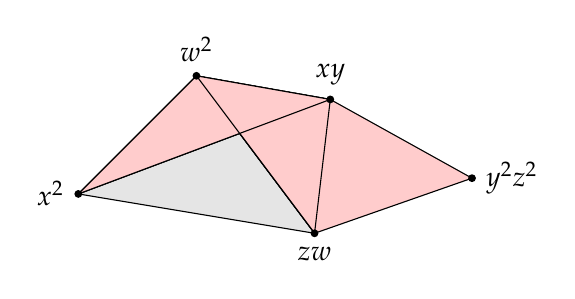
\begin{tikzpicture}[scale=1]

\draw[fill=gray!20] (0,0) -- (3,-0.5) -- (3.2,1.2)-- (0,0); 
\draw[fill=gray!20] (0,0) -- (1.5,1.5) -- (3.2,1.2)-- (0,0); 
\draw[] (1.5,1.5) -- (3,-0.5);

\draw[fill=red!20] (3,-0.5) -- (5,0.2) -- (3.2,1.2);
\draw[fill=red!20] (3,-0.5) -- (1.5,1.5) -- (3.2,1.2);
\draw[] (3,-0.5) -- (3.2,1.2);
\draw[fill=red!20] (0,0) -- (1.5,1.5) -- (3.2,1.2);

\node[circle, fill=black, inner sep=1pt, label=left:$x^2 $] (a) at (0,0) {};
\node[circle, fill=black, inner sep=1pt, label=above:$w^2 $] (b) at (1.5,1.5) {};
\node[circle, fill=black, inner sep=1pt, label=below:$zw $] (c) at (3,-0.5) {};
\node[circle, fill=black, inner sep=1pt, label=above:$xy $] (d) at (3.2,1.2) {}; 
\node[circle, fill=black, inner sep=1pt, label=right:$y^2 z^2 $] (e) at (5,0.2) {};


\draw[color=black!100] (1.5,1.5) -- (3,-0.5);
\draw[color=black!100] (0,0) -- (3.2,1.2);

\end{tikzpicture} \end{center} We now ask: is $\iota'$ an MDG algebra homomorphism? The answer
is no. Indeed, clearly this map is a chain map which fixes the identity
element, however it is not multiplicative. In fact, it's not even
$2$-multiplicative. To see this, assume for a contradiction that
it was $2$-multiplicative. Then we'd have
\begin{align*}
0 & =\iota'(0)\\
 & =\iota'([e_{1}',e_{2}',e_{3}'])\\
 & =[\iota'(e_{1}'),\iota'(e_{2}'),\iota'(e_{3}')]\\
 & =[e_{1},e_{2},e_{5}]\\
 & \neq0,
\end{align*}
which is an obvious contradiction.

\hfill

~~~Next let $\boldsymbol{m}''=x^{2},w^{2},zw,xy$ and let $T''=\mathcal{T}(\boldsymbol{m}'')$
be the Taylor algebra which resolves $R\slash\boldsymbol{m}''$. The
standard homogeneous basis of $T''$ is denoted by $e_{\sigma}''$.
Choose a comparison map $\iota''\colon T''\to F$ which lifts the
projection $R\slash\boldsymbol{m}''\to R\slash\boldsymbol{m}$ such
that $\iota''$ is unital and respects the multigrading. Then $\iota''$
being a chain map together with the fact that it is multigraded forces
us to have $\iota''(e_{\sigma}'')=e_{\sigma}$ for all $\sigma$.
We can picture $\iota''(T'')$ inside of $F$ as being supported on
the red-shaded subcomplex  below: \begin{center}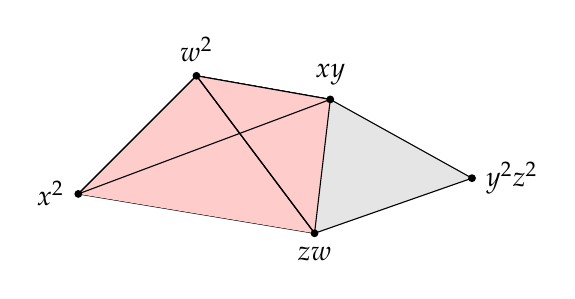
\begin{tikzpicture}[scale=1]

\draw[fill=gray!20] (0,0) -- (3,-0.5) -- (3.2,1.2)-- (0,0); 
\draw[fill=gray!20] (0,0) -- (1.5,1.5) -- (3.2,1.2)-- (0,0); 
\draw[fill=gray!20] (3,-0.5) -- (5,0.2) -- (3.2,1.2);
\draw[] (1.5,1.5) -- (3,-0.5);

\draw[fill=red!20] (0,0) -- (1.5,1.5) -- (3.2,1.2);
\draw[fill=red!20] (3,-0.5) -- (1.5,1.5) -- (3.2,1.2);
\draw[] (3,-0.5) -- (3.2,1.2);
\draw[fill=red!20] (0,0) -- (1.5,1.5) -- (3,-0.5);

\node[circle, fill=black, inner sep=1pt, label=left:$x^2 $] (a) at (0,0) {};
\node[circle, fill=black, inner sep=1pt, label=above:$w^2 $] (b) at (1.5,1.5) {};
\node[circle, fill=black, inner sep=1pt, label=below:$zw $] (c) at (3,-0.5) {};
\node[circle, fill=black, inner sep=1pt, label=above:$xy $] (d) at (3.2,1.2) {}; 
\node[circle, fill=black, inner sep=1pt, label=right:$y^2 z^2 $] (e) at (5,0.2) {};


\draw[color=black!100] (1.5,1.5) -- (3,-0.5);
\draw[color=black!100] (0,0) -- (3.2,1.2);

\end{tikzpicture} \end{center} This time it is easy to check that $\iota''$ is an MDG algebra homomorphism.
We give $F$ the structure of an MDG $T''$-module using $\iota''$
in the usual way. Notice that $F$ is \emph{not }associative as a
$T''$-module, that is $F$ is not a DG $T''$-module. Indeed, we
have $[e_{1},e_{2},e_{5}]\neq0$.

\hfill

~~~Finally let $\boldsymbol{t}=x^{2}+w^{2},w^{2}+xy,x^{2}+zw$.
One can check that $\boldsymbol{t}$ is an $R$-regular sequence contained
in $\langle\boldsymbol{m}\rangle$. Let $E=\mathcal{K}(\boldsymbol{t})$
be the Koszul $R$-algebra which resolve $R\slash\boldsymbol{t}$.
The standard homogeneous basis of $E$ is denoted by $\epsilon_{\sigma}$.
We begin to construct a comparison map $\iota\colon E\to F$ which
lifts the projection $R\slash\boldsymbol{t}\to R\slash\boldsymbol{m}$
by setting
\begin{align*}
\iota(\epsilon_{1}) & =e_{1}+e_{2}\\
\iota(\epsilon_{2}) & =e_{2}+e_{3}\\
\iota(\epsilon_{3}) & =e_{3}+e_{4}
\end{align*}
It is straightforward to check that this extends to a unique MDG algebra
homomorphism by setting
\[
\iota(\epsilon_{\sigma})=\prod_{i\in\sigma}\iota(\epsilon_{i}).
\]
We give $F$ the structure of an MDG $E$-module using $\iota$ in
the usual way. Again, note that $F$ is not a DG $E$-module, however
$\iota\colon E\to F$ \emph{is }an MDG algebra homomorphism. \end{example}

\subsubsection{Multiplicator Identities}

We want to familiarize ourselves with the multiplicator of $\varphi\colon X\to Y$,
so in this subsubsection we collect together some identities which
the multiplicator satisfies:
\begin{itemize}
\item For all $a\in A$ homogeneous and $x\in X$, we have the Leibniz law:
\[
\mathrm{d}[a,x]=[\mathrm{d}a,x]+(-1)^{|a|}[a,\mathrm{d}x].
\]
\item For all $a\in A$ homogeneous and $x\in X$ homogeneous, we have
\begin{equation}
[a,x]=(-1)^{|a||x|}[x,a].\label{eq:identity3-1-1-1}
\end{equation}
\item For all $a_{1},a_{2}\in A$ and $x\in X$, we have
\begin{equation}
a_{1}[a_{2},x]-[a_{1}a_{2},x]+[a_{1},a_{2}x]=[a_{1},a_{2},x]_{\varphi}\label{eq:identity1-1-1-1}
\end{equation}
\end{itemize}
Furthermore, if $Z$ is another MDG $A$-module and $\psi\colon Y\to Z$
is another chain map, then for all $a\in A$ and $x\in X$, we have
\begin{equation}
[a,x]_{\psi\varphi}=\psi([a,x]_{\varphi})+[a,\varphi(x)]_{\psi}\label{eq:identityjklfds}
\end{equation}
In particular, if $\psi$ is multiplicative, then $\psi([Y]_{\varphi})\subseteq[Z]_{\psi\varphi}$.

\begin{rem}\label{rem} Let $A$ and $B$ be MDG $R$-algebras and
let $\varphi\colon A\to B$ be a chain map such that $\varphi(1)=1$.
Then we can rewrite (\ref{eq:identity1-1-1-1}) as follows: for all
$a_{1},a_{2},a_{3}\in A$, we have
\begin{equation}
\varphi(a_{1})[a_{2},a_{3}]-[a_{1}a_{2},a_{3}]+[a_{1},a_{2}a_{3}]-[a_{1},a_{2}]\varphi(a_{3})=[\varphi(a_{1}),\varphi(a_{2}),\varphi(a_{3})]-\varphi([a_{1},a_{2},a_{3}])\label{eq:identity1-1-1}
\end{equation}
Indeed, this follows from the fact that
\[
[\varphi(a_{1}),\varphi(a_{2}),\varphi(a_{3})]=[a_{1},a_{2},\varphi(a_{3})]-[a_{1},a_{2}]\varphi(a_{3}).
\]
In this case, we also have $[a,a]_{\varphi}=0$ for all $a\in A$
where $|a|$ is odd. \end{rem}

\begin{prop}\label{prop} Let $A$ and $B$ be MDG algebras and let
$\varphi\colon A\to B$ be a chain map such that $\varphi(1)=1$.
The multiplicator map $[\cdot]_{\varphi}\colon A^{\otimes2}\to B$
defined by
\[
[a_{1}\otimes a_{2}]_{\varphi}=[a_{1},a_{2}]=a_{1}a_{2}-a_{1}\star a_{2},
\]
where $\cdot$ denotes the multiplication in $B$ and $\star$ denotes
the multiplication in $A$ is strictly graded-commutative. \end{prop}

\begin{proof}\label{proof} Graded-commutativity is clear. To see
why it is associative, observe that
\begin{align*}
[[a_{1},a_{2}],a_{3}]-[a_{1},[a_{2},a_{3}]] & =[a_{1}a_{2},a_{3}]-[a_{1}\star a_{2},a_{3}]-[a_{1},a_{2}a_{3}]+[a_{1},a_{2}\star a_{3}]\\
 & =[a_{1}\star a_{2},a_{3}]-[a_{1},a_{2}\star a_{3}]+[a_{1}a_{2},a_{3}]-[a_{1},a_{2}a_{3}]\\
 & =a_{1}[a_{2},a_{3}]-[a_{1},a_{2}]a_{3}+[a_{1}a_{2},a_{3}]-[a_{1},a_{2}a_{3}]-[a_{1},a_{2},a_{3}]_{\mu}+[a_{1},a_{2},a_{3}]_{\nu}\\
 & =(a_{1}\star a_{2})a_{3}-a_{1}(a_{2}\star a_{3})+a_{1}\star(a_{2}a_{3})-(a_{1}a_{2})\star a_{3}-[a_{1},a_{2},a_{3}]_{\mu}+[a_{1},a_{2},a_{3}]_{\nu}\\
 & =[a_{1},a_{2},a_{3}]_{\mu,\nu}-[a_{1},a_{2},a_{3}]_{\nu,\mu}+[a_{1},a_{2},a_{3}]_{\nu}-[a_{1},a_{2},a_{3}]_{\mu}
\end{align*}
Where we used
\[
a_{1}[a_{2},a_{3}]-[a_{1},a_{2}]a_{3}=[a_{1}\star a_{2},a_{3}]-[a_{1},a_{2}\star a_{3}]+[a_{1},a_{2},a_{3}]_{\mu}-[a_{1},a_{2},a_{3}]_{\nu}
\]

Note that
\begin{align*}
a_{1}[a_{2},a_{3}] & =a_{1}(a_{2}a_{3})-a_{1}(a_{2}\star a_{3})\\{}
[a_{1},a_{2}]a_{3} & =(a_{1}a_{2})a_{3}-(a_{1}\star a_{2})a_{3}\\{}
[a_{1}a_{2},a_{3}] & =(a_{1}a_{2})a_{3}-(a_{1}a_{2})\star a_{3}\\{}
[a_{1},a_{2}a_{3}] & =a_{1}(a_{2}a_{3})-a_{1}\star(a_{2}a_{3})
\end{align*}

Alternatively we have just shown
\[
[\cdot,\cdot,\cdot]_{\nu-\mu}=[\cdot,\cdot,\cdot]_{\nu}-[\cdot,\cdot,\cdot]_{\mu}-[\cdot,\cdot,\cdot]_{\nu,\mu}+[\cdot,\cdot,\cdot]_{\mu,\nu}
\]

\end{proof}

\subsubsection{The Maximal Multiplicative Quotient}

The \textbf{multiplicator complex }of $\varphi$, denoted $[Y]_{\varphi}$,
is the $R$-subcomplex of $Y$ given by $[Y]_{\varphi}:=\mathrm{im}\,[\cdot]_{\varphi}$,
so the underlying graded module of $[Y]_{\varphi}$
\[
[Y]_{\varphi}:=\mathrm{span}_{R}\{[a,x]_{\varphi}\mid a\in A\text{ and }x\in X\},
\]
and the differential of $[Y]_{\varphi}$ is simply the restriction
of the differential of $Y$ to $[Y]_{\varphi}$. In order to avoid
confusion with the associator complex, we will always write $\varphi$
in the subscript of $[Y]_{\varphi}$. Even though the multiplicator
complex of $\varphi$ is closed under the differential, it need not
be closed under $A$-scalar multiplication. In other words, if $a_{1},a_{2}\in A$
and $x\in X$, then it need not be the case that $a_{1}[a_{2},x]_{\varphi}\in[Y]_{\varphi}$.
We denote by $\langle Y\rangle_{\varphi}$ to be the MDG $A$-submodule
of $Y$ generated by $[Y]_{\varphi}$. In other words, $\langle Y\rangle_{\varphi}$
is the smallest MDG $A$-submodule of $Y$ which contains $[Y]_{\varphi}$.
Unlike the associator submodule, the multiplicator submodule is difficult
to describe in terms of an $R$-span of elements. Indeed, as a first
guess, one might think that $\langle Y\rangle_{\varphi}$ is given
by
\begin{equation}
\mathrm{span}_{R}\{[a,x]_{\varphi}\mid a\in A\text{ and }x\in X\}.\label{eq:multiplci-1}
\end{equation}
However this is clearly incorrect in general as we may need to adjoin
elements of the form $a_{1}[a_{2},x]$ to (\ref{eq:multiplci-1}).
As a second guess, one might think that $\langle Y\rangle_{\varphi}$
is given by
\begin{equation}
\mathrm{span}_{R}\{a_{1}[a_{2},x]_{\varphi}\mid a_{1},a_{2}\in A\text{ and }x\in X\}.\label{eq:multiplci}
\end{equation}
However this isn't correct in general either since the identity
\[
a_{1}(a_{2}[a_{3},x]_{\varphi})=(a_{1}a_{2})[a_{3},x]_{\varphi}-[a_{1},a_{2},[a_{3},x]_{\varphi}]
\]
tells us that should really adjoin elements of the form $a_{1}[a_{2},a_{3},[a_{4},x]]$
to (\ref{eq:multiplci}) as well. As a third guess, one might think
that $\langle Y\rangle_{\varphi}$ is given by
\begin{equation}
\mathrm{span}_{R}\{a_{1}[a_{2},x]_{\varphi},\,a_{1}[a_{2},a_{3},[a_{4},x]_{\varphi}]\mid a_{1},a_{2},a_{3},a_{4}\in A\text{ and }x\in X\}.\label{eq:multiplicatorcomplexrspan-1}
\end{equation}
Again this isn't correct in general since the identity
\[
a_{1}(a_{2}[a_{3},a_{4},[a_{5},x]_{\varphi}])=(a_{1}a_{2})[a_{3},a_{4},[a_{5},x]]-[a_{1},a_{2},[a_{3},a_{4},[a_{5},x]_{\varphi}]].
\]
tells us that we should really adjoin elements of the form $a_{1}[a_{2},a_{3},[a_{4},a_{5},[a_{6},x]_{\varphi}]]$
to (\ref{eq:multiplicatorcomplexrspan-1}) as well. The problem continues
getting worse with no end in sight. It turns out however, that if
$\varphi$ is $2$-multiplicative, then $\langle Y\rangle_{\varphi}$
given by (\ref{eq:multiplci-1}).

\begin{prop}\label{prop} If $\varphi$ is $2$-multiplicative, then
for all $a_{1},a_{2},a_{3}\in A$ and $x\in X$ we have
\begin{equation}
a_{1}[a_{2},x]_{\varphi}=[a_{1}a_{2},x]_{\varphi}-[a_{1},a_{2}x]_{\varphi}\quad\text{and}\quad[a_{1},a_{2},[a_{3},x]_{\varphi}]=[[a_{1},a_{2},a_{3}],x]_{\varphi}-[a_{1},[a_{2},a_{3},x]]_{\varphi}.\label{eq:2multiident}
\end{equation}
In particular, $\langle Y\rangle_{\varphi}$ is given by (\ref{eq:multiplci-1}).
\end{prop}

\begin{proof}\label{proof} A straightforward calculation yields
\begin{align*}
a_{1}[a_{2},a_{3},x]_{\varphi} & =[a_{1}a_{2},a_{3},x]_{\varphi}-[a_{1},a_{2}a_{3},x]_{\varphi}+[a_{1},a_{2},a_{3}x]_{\varphi}-[[a_{1},a_{2},a_{3}],x]_{\varphi}+[a_{1},[a_{2},a_{3},x]]_{\varphi}-[a_{1},a_{2},[a_{3},x]_{\varphi}].
\end{align*}
Using this identity together with the identity (\ref{eq:identity1-1-1-1}),
we see that if $\varphi$ is $2$-multiplicative, then we obtain (\ref{eq:2multiident}).
This implies all elements of the form $a_{1}[a_{2},x]$ and $a_{1}[a_{2},a_{3},[a_{4},x]]$
belong to (\ref{eq:multiplci-1}). An easy induction argument shows
that $\langle Y\rangle_{\varphi}$ is given by (\ref{eq:multiplci-1}).
\end{proof}

~~~The quotient $Y\slash\langle Y\rangle_{\varphi}$ is an MDG
$A$-module. We denote by $\pi\colon Y\to Y\slash\langle Y\rangle_{\varphi}$
to be the canonical quotient map. Note that both $\pi$ and $\pi\varphi$
are multiplicative. Therefore (\ref{eq:identityjklfds}) implies $[Y]_{\varphi}\subseteq\ker\pi$
which implies $\langle Y\rangle_{\varphi}\subseteq\ker\pi$. We call
$Y\slash\langle Y\rangle_{\varphi}$ (together with its canonical
quotient map $\pi$) the \textbf{maximal multiplicative quotient }of\textbf{
}$\varphi\colon X\to Y$; it satisfies the following universal mapping
property: 

\begin{prop}\label{prop} For all MDG $A$-modules $Z$ and for all
chain maps $\psi\colon Y\to Z$ where both $\psi$ and $\psi\varphi$
are MDG $A$-module homomorphisms (hence both are multiplicative),
there exists a unique MDG $A$-module homomorphism $\overline{\psi}\colon Y\slash\langle Y\rangle_{\varphi}\to Z$
such that $\overline{\psi}\pi=\psi$. We express this in terms of
a commutative diagram as below:

\begin{equation}\label{equationump2}\begin{tikzcd}[row sep =40, column sep = 40]  X \arrow[r, " \varphi "] & Y \arrow[d, " \pi "] \arrow[dl, "\psi ",swap] \\ Z  & Y \slash \langle Y \rangle _{ \varphi } \arrow[l," \overline{\psi }",dashed] \end{tikzcd}\end{equation}

\end{prop}\begin{proof}\label{proof} Suppose $\psi\colon Y\to Z$
is such a map. Then (\ref{eq:identityjklfds}) implies $[Y]_{\varphi}\subseteq\ker\psi$
which implies $\langle Y\rangle_{\varphi}\subseteq\ker\psi$. Thus
the map $\overline{\psi}\colon Y\slash\langle Y\rangle_{\varphi}\to Z$
given by
\[
\overline{\psi}(\overline{y}):=\psi(y),
\]
where $\overline{y}\in Y\slash\langle Y\rangle_{\varphi}$ and where
$y\in Y$ is a choice of an element in $Y$ such that $\pi(y)=\overline{y}$,
is well-defined. Furthermore, it is easy to check that $\overline{\psi}$
is an MDG $A$-module homomorphism and the unique such map which makes
the diagram (\ref{equationump2}) commute. \end{proof}

\begin{rem}\label{rem} Let $[a_{1},a_{2}]=a_{1}a_{2}-a_{1}\star a_{2}$.
Observe that

\end{rem}

\section{The Symmetric DG Algebra}

Let $R$ be a commutative ring, let $A$ be a $\mathbb{Z}$-graded
$R$-module such that $A_{0}=R$ which is also equipped with a $\mathbb{Z}$-linear
differential $\mathrm{d}\colon A\to A$ giving it the structure of
a chain complex. Note that that the differential need not be $R$-linear
and note that $A$ may be nonzero in negative homological degree.
In this section, we will construct the symmetric DG algebra of $A$,
which we denote by $\mathrm{S}(A)=\mathrm{S}$ (where we omit $A$
from the notation when context is clear). After constructing the symmetric
DG algebra in this general setting, we then specialize to the case
we are mostly interesting in: we say $A$ is \textbf{centered }at\textbf{
$R$} if $A$ is an $R$-complex with $A_{0}=R$ and $A_{<0}=0$ (in
particular the differential of $A$ is $R$-linear). In this case,
we sometimes denote the symmetric DG algebra of $A$ by $\mathrm{S}_{R}(A)$
with $R$ in the subscript in order to emphasize that $A$ is centered
at $R$. 

~~~Before we give a rigorous construction of the symmetric DG algebra,
we wish to help motivate the reader by giving an informal description
of it in this special case where $A$ is centered at $R$. In this
case, the underlying graded algebra of $\mathrm{S}=\mathrm{S}_{R}(A)$
is the usual symmetric $R$-algebra $\mathrm{Sym}(A_{+})$ where we
view $A_{+}$ as just an $R$-module. However $\mathrm{S}$ obtains
a bi-graded structure using homological degree and total degree: we
have a decomposition of $\mathrm{S}$ into $R$-modules:
\[
\mathrm{S}=\bigoplus_{i\geq0}\mathrm{S}_{i}=\bigoplus_{m\geq0}\mathrm{S}^{m}=\bigoplus_{i,m\geq0}\mathrm{S}_{i}^{m}.
\]
We refer to the $i$ in the subscript as homological degree\textbf{
}and we refer to the $m$ in the superscript as total degree. We have
\[
\mathrm{S}_{0}=\mathrm{S}^{0}=\mathrm{S}_{0}^{0}=R\quad\text{and}\quad\mathrm{S}^{1}=A_{+}.
\]
More generally, for $i,m\geq1$, the $R$-module $\mathrm{S}_{i}^{m}$
is the $R$-span of all homogeneous elementary products of the form
$\boldsymbol{a}=a_{1}\cdots a_{m}$ where $a_{1},\dots,a_{m}\in A_{+}$
are homogeneous (with respect to homological degree of course) such
that
\[
|\boldsymbol{a}|=|a_{1}|+\cdots+|a_{m}|=i.
\]
In particular, note that $A=\mathrm{S}^{\leq1}=R+A_{+}$, thus we
may (and do) view $A$ a sitting inside $\mathrm{S}$. The differential
of $\mathrm{S}$ extends the differential of $A$ in a natural way
and is defined on homogeneous elementary products $\boldsymbol{a}=a_{1}\cdots a_{m}$
by
\begin{align}
\mathrm{d}\boldsymbol{a} & =\sum_{j=1}^{m}(-1)^{|a_{1}|+\cdots+|a_{j-1}|}a_{1}\cdots\mathrm{d}(a_{j})\cdots a_{m}.\label{eq:caretaken}
\end{align}
If each of the $a_{j}$ in (\ref{eq:caretaken}) live in homological
degree $\ge2$, then $\mathrm{d}\boldsymbol{a}$ and $\boldsymbol{a}$
has the same total degree, namely $\deg(\mathrm{d}\boldsymbol{a})=m=\deg\boldsymbol{a}$.
However if one of the $a_{j}$ in (\ref{eq:caretaken}) lives in homological
degree $1$, then $\deg(\mathrm{d}\boldsymbol{a})=m-1$. The diagram
below illustrates how the differential acts on the bi-graded components:
\begin{center}\begin{tikzcd}[column sep = 7] 


A_i \arrow[dr] && \cdots \arrow[dl] \arrow[dr] && \mathrm{S}_i ^{m-1} \arrow[dl] \arrow[dr] && \mathrm{S}_i ^{m}  \arrow[dl] \arrow[dr] &&  \mathrm{S}_i ^{m+1} \arrow[dl] \arrow[dr] && \cdots \arrow[dl] \arrow[dr] && \mathbb{K} _i \arrow[dl]

\\

& A_{i-1} && \mathrm{S}_{i-1} ^{m-2}   && \mathrm{S}_{i-1} ^{m-1}  && \mathrm{S}_{i-1} ^{m} && \mathrm{S}_{i-1} ^{m+1} && \mathbb{K} _{i-1}



\end{tikzcd}\end{center}where we set $\mathbb{K}$ to be the koszul DG algebra induced by
$\mathrm{d}\colon A_{1}\to A_{0}$. Thus the differential of $\mathrm{S}$
connects the usual differential of $A$ on the far left to a koszul
differential on the far right. In order to keep track of how the differential
operates on the bi-graded components, we express $\mathrm{d}$ as
\[
\mathrm{d}=\eth+\partial,
\]
where $\eth$ is the component of $\mathrm{d}$ which respects total
degree and where $\partial$ is the component of $\mathrm{d}$ which
drops total degree by $1$. In the next example, we consider a free
resolution of a cyclic module and work out what the symmetric DG algebra
looks like in this case.

\begin{example}\label{example} Let $R=\Bbbk[x,y]$, let $I=\langle x^{2},xy\rangle$,
and let $F$ be Taylor resolution of $R\slash I$. Let's write down
the homogeneous components of $F$ as a graded $R$-module as well
as how the differential acts on the homogeneous basis:
\begin{align*}
F_{0} & =R & \mathrm{d}e_{1} & =x^{2}\\
F_{1} & =Re_{1}+Re_{2} & \mathrm{d}e_{2} & =xy\\
F_{2} & =Re_{12}, & \mathrm{d}e_{12} & =xe_{2}-ye_{1},
\end{align*}
Note that the Taylor resolution usually comes equipped with a multiplication
called the Taylor multiplication. Let us denote this by $\star$ so
as not to confuse it with the multiplication $\cdot$ of $\mathrm{S}=\mathrm{S}_{R}(F)$.
Now let's write down the homogeneous components of $\mathrm{S}$ as
a graded $R$-module (with respect to homological degree): we have
\begin{align*}
\mathrm{S}_{0} & =R\\
\mathrm{S}_{1} & =Re_{1}+Re_{2}\\
\mathrm{S}_{2} & =Re_{12}+Re_{1}e_{2}\\
\mathrm{S}_{3} & =Re_{1}e_{12}+Re_{2}e_{12}\\
\mathrm{S}_{4} & =Re_{12}^{2}+Re_{1}e_{2}e_{12}\\
 & \vdots
\end{align*}
Thus we see that $\mathrm{S}$ is much larger than $F$. Note that
$\mathrm{S}_{4}^{3}=Re_{1}e_{2}e_{12}$ and $\mathrm{S}_{4}^{2}=Re_{12}^{2}$.
Also note that
\begin{align*}
\mathrm{d}(e_{1}e_{2}-e_{1}\star e_{2}) & =\mathrm{d}(e_{1}e_{2}-xe_{12})\\
 & =\mathrm{d}(e_{1})e_{2}-e_{1}\mathrm{d}(e_{2})-x\mathrm{d}(e_{12})\\
 & =x^{2}e_{2}-xye_{1}-x(xe_{2}-ye_{1})\\
 & =x^{2}e_{2}-xye_{1}-x^{2}e_{2}+xye_{1}\\
 & =0.
\end{align*}
In fact, we claim that $f_{12}:=e_{1}e_{2}-xe_{12}$ represents a
nonzero element in $\mathrm{H}_{2}(\mathrm{S})$. To see this, note
that $f_{12}$ lives in $\mathrm{S}_{2}^{1}\oplus\mathrm{S}_{2}^{2}$.
Therefore if $\mathrm{d}f=f_{12}$, then $f$ must live in $\mathrm{S}_{3}^{2}=Re_{1}e_{12}+Re_{2}e_{12}$
since $\mathrm{S}_{3}^{1}=0=\mathrm{S}_{3}^{3}$ . However a calculation
shows
\begin{align*}
\mathrm{d}(e_{1}e_{12}) & =x^{2}e_{12}-e_{1}(xe_{2}-ye_{1})=xf_{12}\\
\mathrm{d}(e_{2}e_{12}) & =xye_{12}-e_{2}(xe_{2}-ye_{1})=yf_{12}.
\end{align*}
In particular we see that $\mathrm{H}_{2}(\mathrm{S})=\Bbbk\overline{f}_{12}$.
\end{example}

\subsection{Construction of the Symmetric DG Algebra of $A$}

We now provide a rigorous construction of $\mathrm{S}(A)=\mathrm{S}$
in the general case where the differential of $A$ need not be $R$-linear
and where $A_{<0}$ is not necessarily zero. Our construction will
occur in three steps:

\hfill

\textbf{Step 1: }We define the \textbf{non-unital} \textbf{tensor
DG algebra} of $A$ to be
\[
\mathrm{U}(A)=\mathrm{U}:=\bigoplus_{n=1}^{\infty}A^{\otimes n},
\]
where the tensor product is taken as $\mathbb{Z}$-complexes. An elementary
tensor in $\mathrm{U}$ is denoted $\boldsymbol{a}=a_{1}\otimes\cdots\otimes a_{n}$
where $a_{1},\dots,a_{n}\in A$ and $n\ge1$. The differential of
$\mathrm{U}$ is denoted by $\mathrm{d}$ again to simplify notation
and is defined on $\boldsymbol{a}$ by
\[
\mathrm{d}\boldsymbol{a}=\sum_{j=1}^{n}(-1)^{|a_{1}|+\cdots+|a_{j-1}|}a_{1}\otimes\cdots\otimes\mathrm{d}a_{j}\otimes\cdots\otimes a_{n}.
\]

We say\textbf{ $\boldsymbol{a}$} is a homogeneous elementary tensors
if each $a_{i}$ is a homogeneous element in $A$. In this case, we
set
\[
|\boldsymbol{a}|=\sum_{i=1}^{n}|a_{i}|\quad\text{and}\quad\deg\boldsymbol{a}=\sum_{i=1}^{n}\deg a_{i},
\]
where $\deg$ is defined on elements $a\in A$ by
\[
\deg a=\begin{cases}
1 & \text{if }a\in A_{>0}\\
0 & \text{if }a\in R\\
-1 & \text{if }a\in A_{<0}
\end{cases}
\]
We call $|\boldsymbol{a}|$ the \textbf{homological degree }of $\boldsymbol{a}$
and we call $\deg\boldsymbol{a}$ the \textbf{total degree }of $\boldsymbol{a}$.
With $|\cdot|$ and $\deg$ defined, we observe that $\mathrm{U}$
admits a bi-graded decomposition:
\[
\mathrm{U}=\bigoplus_{i\in\mathbb{Z}}\mathrm{U}_{i}=\bigoplus_{m\in\mathbb{Z}}\mathrm{U}^{m}=\bigoplus_{i,m\in\mathbb{Z}}\mathrm{U}_{i}^{m},
\]
where the component $\mathrm{U}_{i}^{m}$ consists of all finite $\mathbb{Z}$-linear
combinations of homogeneous elementary tensors $\boldsymbol{a}\in\mathrm{U}$
such that $|\boldsymbol{a}|=i$ and $\deg\boldsymbol{a}=m$. We equip
$\mathrm{U}$ with an associative (but not commutative nor unital)
bi-graded $\mathbb{Z}$-bilinear multiplication which is defined on
homogeneous elementary tensors by $(\boldsymbol{a},\boldsymbol{a}')\mapsto\boldsymbol{a}\otimes\boldsymbol{a}'$
and is extended $\mathbb{Z}$-bilinearly everywhere else. This multiplication
is easily seen to satisfy Leibniz law, however note that $\mathrm{U}$
is not unital under this multiplication since $(1,1)\mapsto1\otimes1\neq1$
(hence why we call this the \emph{non-unital }tensor DG algebra).
Also note that $\mathrm{U}$ already comes equipped with an $R$--scalar
multiplication (from the $R$-module structure on $A$), denoted $(r,\boldsymbol{a})\mapsto r\boldsymbol{a}$,
however the multiplication of $\mathrm{U}$ only agrees with the $R$-scalar
multiplication wherever they are both defined and vanish. Let $\mathfrak{u}$
to be the $\mathrm{U}$-ideal by all elements of the form
\begin{align*}
[r,a]_{\mu} & =r\otimes a-ra & [a,r]_{\mu} & =a\otimes r-ar\\{}
[r,a]_{\mathrm{d}} & =\mathrm{d}r\otimes a-\mathrm{d}(ra)+r(\mathrm{d}a) & [a,r]_{\mathrm{d}} & =(-1)^{|a|}a\otimes\mathrm{d}r-\mathrm{d}(ar)+(\mathrm{d}a)r
\end{align*}
where $r\in R$ and $a\in A$. We claim that the differential of $\mathrm{U}$
maps $\mathfrak{u}$ to itself. Indeed, given $r\in R$ and $a\in A$,
we have
\begin{align*}
\mathrm{d}[r,a]_{\mu} & =\mathrm{d}(r\otimes a)-\mathrm{d}(ra)\\
 & =\mathrm{d}r\otimes a+r\otimes\mathrm{d}a-\mathrm{d}r\otimes a+r(\mathrm{d}a)+[r,a]_{\mathrm{d}}\\
 & =r\otimes\mathrm{d}a+r(\mathrm{d}a)+[r,a]_{\mathrm{d}}\\
 & =[r,\mathrm{d}a]_{\mu}+[r,a]_{\mathrm{d}}\\
 & \in\mathfrak{u}.
\end{align*}
Similarly we have
\begin{align*}
\mathrm{d}[r,a]_{\mathrm{d}} & =\mathrm{d}(\mathrm{d}r\otimes a-\mathrm{d}(ra)+r(\mathrm{d}a))\\
 & =-\mathrm{d}r\otimes\mathrm{d}a+\mathrm{d}(r(\mathrm{d}a))\\
 & =-\mathrm{d}r\otimes\mathrm{d}a+\mathrm{d}(r\otimes\mathrm{d}a-[r,\mathrm{d}a]_{\mu})\\
 & =-\mathrm{d}r\otimes\mathrm{d}a+\mathrm{d}r\otimes\mathrm{d}a-\mathrm{d}[r,\mathrm{d}a]_{\mu}\\
 & =-\mathrm{d}[r,\mathrm{d}a]_{\mu}\\
 & =-[r,\mathrm{d}a]_{\mathrm{d}}\\
 & \in\mathfrak{u}.
\end{align*}
Similar calculations show $\mathrm{d}[a,r]_{\mu}\in\mathfrak{u}$
and $\mathrm{d}[r,a]_{\mathrm{d}}\in\mathfrak{u}$. 

\hfill

\textbf{Step 2: }We define the \textbf{tensor DG algebra }of $A$
to be the quotient
\[
\mathrm{T}(A)=\mathrm{T}:=\mathrm{U}\slash\mathfrak{u}.
\]

The multiplication of $\mathrm{U}$ induces a multiplication on $\mathrm{T}$
which not only becomes unital but also agrees with the $R$-scalar
multiplication on $\mathrm{T}$ where they are both defined. Since
$\mathfrak{u}$ is generated by elements which are homogeneous with
respect to homological degree and since the differential of $\mathrm{U}$
maps $\mathfrak{u}$ to itself, it follows that the differential of
$\mathrm{U}$ induces a differential on $\mathrm{T}$, which we again
denote by $\mathrm{d}$ again. This gives $\mathrm{T}$ the structure
of a non-commutative (but unital) DG $\Bbbk$-algebra, where
\[
\Bbbk=\{r\in R\mid\mathrm{d}r\otimes a=0\text{ for all }a\in A\}.
\]
In other words, the differential of $\mathrm{T}$ satisfies Leibniz
law and is $\Bbbk$-linear. Note that the generators $[r,a]_{\mu}$
of $\mathfrak{u}$ is also homogeneous with respect to total degree,
however the generator $[r,a]_{\mathrm{d}}$ is homogeneous with respect
to total degree if and only if either $\mathrm{d}r\otimes a=0$, or
$\mathrm{d}(ra)=r\mathrm{d}a$, or $|a|\in\{0,1\}$. In particular,
$\mathfrak{u}$ will be homogeneous with respect to total degree if
$A$ is centered at $R$ (which is a case we are interested in). In
this case, $\mathrm{T}$ inherits from $\mathrm{U}$ a bi-graded $R$-algebra
structure:
\[
\mathrm{T}=\bigoplus_{i\in\mathbb{Z}}\mathrm{T}_{i}=\bigoplus_{m\in\mathbb{Z}}\mathrm{T}^{m}=\bigoplus_{i,m\in\mathbb{Z}}\mathrm{T}_{i}^{m}.
\]
If we assume in addition that the differential of $A$ is $R$-linear
to begin with, then we have 
\[
\mathrm{T}_{0}=\mathrm{T}^{0}=\mathrm{T}_{0}^{0}=R\quad\text{and}\quad\mathrm{T}^{1}=A_{+}.
\]
More generally, for $i,m\geq1$ the component $\mathrm{T}_{i}^{m}$
consists of all finite $R$-linear combinations of homogeneous elementary
tensors of the form $\boldsymbol{a}=a_{1}\otimes\cdots\otimes a_{m}$
where $a_{1},\dots,a_{m}\in A_{+}$ and where $|\boldsymbol{a}|=i$.

\begin{example}\label{example} Let us describe what the total degree
$m$ component of $\mathrm{T}$ looks like in the case where the differential
of $A$ is $R$-linear and where $A_{<0}=0$. We have
\begin{align*}
\mathrm{T}^{0} & =R\\
\mathrm{T}^{1} & =\bigoplus_{1\leq i}A_{i}\\
\mathrm{T}^{2} & =\bigoplus_{\substack{1\leq i<j}
}((A_{i}\otimes A_{j})\oplus(A_{j}\otimes A_{i}))\oplus\bigoplus_{1\leq i}A_{i}^{\otimes2}
\end{align*}
The component $\mathrm{T}^{3}$ is slightly more complicated:
\[
\bigoplus_{\substack{1\leq i<j<k\\
\pi\in S_{3}
}
}(A_{\pi(i)}\otimes A_{\pi(j)}\otimes A_{\pi(k)})\oplus\bigoplus_{\substack{1\leq i<j\\
\pi\in S_{2}
}
}((A_{\pi(i)}^{\otimes2}\otimes A_{\pi(j)})\oplus(A_{\pi(i)}\otimes A_{\pi(j)}\otimes A_{\pi(i)})\oplus(A_{\pi(i)}\otimes A_{\pi(j)}^{\otimes2}))\oplus\bigoplus_{1\leq i}A_{i}^{\otimes3}.
\]

\end{example}

We set $\mathfrak{t}$ to be the $\mathrm{T}$-ideal generated by
all elements of the form
\[
[a_{1},a_{2}]_{\sigma}\colon=(-1)^{|a_{1}||a_{2}|}a_{2}\otimes a_{1}-a_{1}\otimes a_{2}\quad\text{and}\quad[a]_{\tau}:=a\otimes a,
\]
where $a,a_{1},a_{2}\in A$ are homogeneous and $|a|$ is odd. Observe
that $\mathrm{d}$ maps $\mathfrak{t}$ to itself since if $a,a_{1},a_{2}\in A$
are homogeneous with $|a|$ odd, then we have
\begin{align*}
\mathrm{d}[a_{1},a_{2}]_{\sigma} & =[\mathrm{d}a_{1},a_{2}]_{\sigma}+(-1)^{|a_{1}|}[a_{1},\mathrm{d}a_{2}]_{\sigma}\in\mathfrak{t}\quad\text{and}\quad\mathrm{d}[a]_{\tau}=[\mathrm{d}a,a]_{\sigma}\in\mathfrak{t}
\end{align*}

\hfill

\textbf{Step 3: }We define the \textbf{symmetric DG algebra }of $A$
to be the quotient
\[
\mathrm{S}(A)=\mathrm{S}:=\mathrm{T}\slash\mathfrak{t}
\]
The image of a homogeneous elementary tensor $a_{1}\otimes\cdots\otimes a_{m}$
in $\mathrm{S}$ is often denoted $a_{1}\cdots a_{n}$ and is called
a homogeneous elementary product. Since $\mathfrak{t}$ is generated
by elements which are homogeneous with respect to both homological
degree and since the differential of $\mathrm{T}$ maps $\mathfrak{t}$
to itself, we see that the differential of $\mathrm{T}$ induces a
differential on $\mathrm{S}$, which we again denote by $\mathrm{d}\colon\mathrm{S}\to\mathrm{S}$,
giving it the structure of a strictly graded-commutative DG $\Bbbk$-algebra.
Furthemore, if $\mathrm{T}$ inherits the bi-graded structure from
$\mathrm{U}$, then $\mathrm{S}$ inherits from $\mathrm{T}$ the
bi-graded structure from $\mathrm{T}$ since $\mathfrak{t}$ is generated
by elements which are homogeneous with respect to total degree. 

\subsection{The Symmetric DG $R$-Algebra}

We now focus our attention to the case where $A$ is an $R$-complex
centered at $R$ and we wish to study $\mathrm{S}=\mathrm{S}_{R}(A)$
the symmetric DG $R$-algebra of $A$. Then $\mathrm{S}$ is also
centered at $R$. In fact, the underlying graded $R$-algebra of $\mathrm{S}$
is the usual symmetric algebra of $A_{+}$:
\[
\mathrm{Sym}(A_{+})=\mathrm{Sym}_{R}(A_{+})=\frac{\bigoplus_{m\ge0}A_{+}^{\otimes m}}{\langle\{[a_{1},a_{2}]_{\sigma},[a]_{\tau}\}\rangle},
\]
where we view $A_{+}$ as just a graded $R$-module and where the
tensor product is taken as graded $R$-modules. 

\subsubsection{Properties of the Symmetric DG $R$-Algebra}

The symmetric DG $R$-algebra construction enjoys the following properties:

\begin{prop}\label{prop} Let $R$ be a commutative ring and let $A$
be an $R$-complex centered at $R$. 
\begin{enumerate}
\item (Universal Mapping Property) For every chain map of the form $\varphi\colon A\to A'$,
where $A'$ is a DG algebra centered at a ring $R'$ and where $\varphi$
restricts to a ring homomorphism $\varphi_{0}\colon R\to R'$, there
exists a unique DG algebra homomorphism $\widetilde{\varphi}\colon\mathrm{S}_{R}(A)\to A'$
which extends $\varphi\colon A\to A'$, that is, such that $\widetilde{\varphi}\circ\iota=\varphi$
where $\iota\colon A\hookrightarrow\mathrm{S}$ is the inclusion map.
We express this in terms of a commutative diagram as below:\begin{equation}\label{equationump2}\begin{tikzcd}[row sep =40, column sep = 40]  A \arrow[dr,"\varphi ", swap] \arrow[r, " \iota ", hook  ] & \mathrm{S}_R (A) \arrow[d, "  \widetilde { \varphi }  " ] \\ & A' \end{tikzcd}\end{equation}
\item (Base Change) Let $R'$ be an $R$-algebra. Then
\[
\mathrm{S}_{R}(A)\otimes_{R}R'=\mathrm{S}_{R'}(A\otimes_{R}R').
\]
\item (Direct Sums) 
\item (Short Exact Sequences) Let \begin{equation}\label{equation}\begin{tikzcd} B \arrow[r] &  A \arrow[r] &  A' \arrow[r] & 0 \end{tikzcd}\end{equation}be
an exact sequence of $R$-complexes where $A'$ is centered at a cyclic
$R$-algebra, say $R'=R\slash I$ for some ideal $I$ of $R$. Then
we obtain an exact sequence\begin{equation}\label{equation}\begin{tikzcd} \mathrm{S}_R (A) \otimes _R B \arrow[r] &  \mathrm{S}_R (A) \arrow[r] &  \mathrm{S}_{R'} (A') \arrow[r] & 0 \end{tikzcd}\end{equation}.
\end{enumerate}
\end{prop}

\begin{proof}\label{proof} 1) Let $\varphi\colon A\to A'$ be such
a chain map and denote $\mathrm{S}=\mathrm{S}_{R}(A)$. We define
$\widetilde{\varphi}\colon\mathrm{S}\to A'$ by setting $\widetilde{\varphi}|_{A}=\varphi$
and
\begin{equation}
\widetilde{\varphi}(a_{1}\cdots a_{m})=\varphi(a_{1})\cdots\varphi(a_{m})\label{eq:satisfythis-1}
\end{equation}
for all homogeneous elementary products $a_{1}\cdots a_{m}$ in $\mathrm{S}^{\geq2}$
and then extending it $R$-linearly everywhere else. By construction,
$\widetilde{\varphi}$ is multiplicative and extends $\varphi\colon A\to A'$.
Furthermore, $\widetilde{\varphi}$ is a chain map since it is a graded
$R$-linear map which commutes with the differential. Indeed, we clearly
have $\widetilde{\varphi}\mathrm{d}(1)=0=\mathrm{d}\widetilde{\varphi}(1)$,
and for all homogeneous elementary products $a_{1}\cdots a_{m}$ in
$\mathrm{S}^{\ge2}$, we have
\begin{align*}
\widetilde{\varphi}\mathrm{d}(a_{1}\cdots a_{m}) & =\sum_{j=1}^{m}(-1)^{|a_{1}|+\cdots+|a_{j-1}|}\widetilde{\varphi}(a_{1}\cdots\mathrm{d}(a_{j})\cdots a_{m})\\
 & =\sum_{j=1}^{m}(-1)^{|a_{1}|+\cdots+|a_{j-1}|}\varphi(a_{1})\cdots\varphi\mathrm{d}(a_{j})\cdots\varphi(a_{m})\\
 & =\sum_{j=1}^{m}(-1)^{|a_{1}|+\cdots+|a_{j-1}|}\varphi(a_{1})\cdots\mathrm{d}\varphi(a_{j})\cdots\varphi(a_{m})\\
 & =\mathrm{d}(\varphi(a_{1})\cdots\varphi(a_{m}))\\
 & =\mathrm{d}\widetilde{\varphi}(a_{1}\cdots a_{m}).
\end{align*}
Finally, if $\widehat{\varphi}\colon\mathrm{S}\to A'$ were another
DG algebra homomorphism which extended $\varphi\colon A\to B$, then
we'd have
\[
\widetilde{\varphi}(a_{1}\cdots a_{m})=\widehat{\varphi}(a_{1})\cdots\widehat{\varphi}(a_{m})=\varphi(a_{1})\cdots\varphi(a_{m})=\widetilde{\varphi}(a_{1}\cdots a_{m})
\]
for all homogeneous elementary products $a_{1}\cdots a_{m}$ in $\mathrm{S}^{\ge2}$,
which implies $\widehat{\varphi}=\widetilde{\varphi}$.

\hfill

2. Note that the underlying graded $R$-algebra of $\mathrm{S}$ is
the usual symmetric of $A_{+}$:
\[
\mathrm{Sym}_{R}(A_{+})=\frac{\bigoplus_{m\ge0}A_{+}^{\otimes m}}{\langle\{[a_{1},a_{2}]_{\sigma},[a]_{\tau}\}\rangle},
\]
where the tensor product is taken as graded $R$-modules.

\end{proof}

\subsubsection{A Presentation of the Maximal Associative Quotient}

We now equip $A$ with a multiplication $(\mu,\star)$ giving it the
structure of an MDG $R$-algebra. In particular, note that if $a_{1},a_{2}\in A_{1}$,
then
\[
a_{1}a_{2}\in\mathrm{S}_{2}^{2},\,\,\,a_{1}\star a_{2}\in\mathrm{S}_{2}^{1},\,\,\,\text{and}\,\,\,[a_{1},a_{2}]\in\mathrm{S}_{2},
\]
where $[a_{1},a_{2}]=a_{1}\star a_{2}-a_{1}a_{2}$ is the multiplicator
of the inclusion map $\iota\colon A\hookrightarrow\mathrm{S}$ evaluated
at $(a_{1},a_{2})\in A^{2}$. Let $\mathfrak{s}=\mathfrak{s}(\mu)$
be the $\mathrm{S}$-ideal generated by all such multiplicators, so
\[
\mathfrak{s}=\mathrm{span}_{\mathrm{S}}\{[a_{1},a_{2}]\mid a_{1},a_{2}\in A\}.
\]
Also let $\pi\colon\mathrm{S}\to\mathrm{S}\slash\mathfrak{s}$ and
$\pi^{\mathrm{as}}\colon A\twoheadrightarrow A^{\mathrm{as}}$ denote
the canonical quotient maps. The universal mapping property of the
symmetric DG $R$-algebra of $A$ implies $\pi^{\mathrm{as}}\colon A\twoheadrightarrow A^{\mathrm{as}}$
extends uniquely to a DG algebra homomorphism $\mathrm{S}\twoheadrightarrow A^{\mathrm{as}}$
which we again denote by $\pi^{\mathrm{as}}$. We let $\mathrm{S}^{\geq2}=\mathrm{S}\slash A$
be the complex whose underlying graded $R$-module is $\mathrm{S}^{\geq2}$
and whose differential $\mathrm{d}^{\geq2}$ is defined by
\[
\mathrm{d}^{\geq2}|_{\mathrm{S}^{m}}=\begin{cases}
\eth|_{\mathrm{S}^{2}} & \text{if }m=2\\
\mathrm{d}|_{\mathrm{S}^{m}} & \text{if }m>2.
\end{cases}
\]
We also let $\rho\colon\mathrm{S}\twoheadrightarrow S\slash A=\mathrm{S}^{\geq2}$
be the canonical quotient map. 

\begin{theorem}\label{theorempresentationsym} With the notation as
above, we have
\[
A^{\mathrm{as}}=\mathrm{coker}(\mathfrak{s}\hookrightarrow\mathrm{S})=\mathrm{S}\slash\mathfrak{s}
\]
More specifically, there is a unique isomorphism $A^{\mathrm{as}}\to\mathrm{S}\slash\mathfrak{s}$
of $\mathrm{DG}$ $\mathrm{S}$-algebras (thus we are justified in
writing $\rho\colon\mathrm{S}\to A^{\mathrm{as}}$ to denote both
$\rho^{\mathrm{as}}\colon\mathrm{S}\to A^{\mathrm{as}}$ and $\rho\colon\mathrm{S}\to\mathrm{S}\slash\mathfrak{s}$
in order to simplify notation) In particular, this implies
\[
\langle A\rangle=A\cap\mathfrak{s}=\mathfrak{s}^{\leq1}=\ker(\mathfrak{s}\to S^{\geq2})
\]
Thus we have the following canonically defined hexagonal-shaped diagram
which is exact everywhere (in every direction) and which is natural
in $A=(A,\mathrm{d},\mu)$:\begin{equation}\label{canondiagram}\begin{tikzcd}[row sep=30 ]& \mathrm{S} ^{\geq 2} \arrow[r] & 0 \\ \mathfrak{s} \arrow[ur, two heads ]  \arrow[r, hook, "i "] & \mathrm{S} \arrow[u, two heads, "\rho ", swap ] \arrow[r, two heads, "\pi "] & A^{\mathrm{as}}  \arrow[u] \\ \mathfrak{s} ^{\leq 1} \arrow[r, hook] \arrow[u, hook' ] & A \arrow[u, hook, "\iota ", swap] \arrow[ur, two heads]\end{tikzcd}\end{equation}In
particular, if $\mathrm{H}_{+}(A)=0$, then $\mathrm{H}_{+}(\mathrm{S})=\mathrm{H}(\mathrm{S}^{\geq2})$
and we obtain a canonically defined sequence of graded $\mathrm{H}(\mathrm{S})$-modules:
\begin{equation}\label{fundamentalsequence}\begin{tikzcd}  \mathrm{H} _{+ }(\mathfrak{s} ) \arrow[r] & \mathrm{H} ( \mathrm{S} ^{\geq 2} ) \arrow[r] & \mathrm{H}_{+ }(A^{\mathrm{as}}) \arrow[r, " \partial " ]  & \Sigma \mathrm{H} (\mathfrak{s} )  \arrow[r] & \Sigma  \mathrm{H} ( \mathrm{S} )  \end{tikzcd}\end{equation}which
is natural in $A=(A,\mathrm{d},\mu)$. \end{theorem}

\begin{rem}\label{rem} By ``natural in $A=(A,\mathrm{d},\mu)$''
we mean that if $R'$ is an $R$-algebra and $\varphi\colon A\to A'$
is an MDG $R$-algebra homomorphism where $A'=(A',\mathrm{d}',\mu')$
is an MDG $R'$-algebra centered at $R'$, then we obtain canonically
defined maps $\mathrm{S}\to\mathrm{S}'$ and $\mathfrak{s}\to\mathfrak{s}'$,
where we set $\mathrm{S}'=\mathrm{S}_{R'}(A')$ and $\mathfrak{s}'=\mathfrak{s}(\mu')$,
which induces a map of diagrams in which everything commutes. For
instance, if $\mathrm{H}_{+}(A)=0=\mathrm{H}_{+}(A')$, then then
we have a commutative diagram of graded $\mathrm{H}(\mathrm{S}')$-modules
of the form:\begin{equation}\label{fundamentalequationtwo}\begin{tikzcd} \mathrm{H}_{ +}(\mathfrak{s} ) \arrow[r] \arrow[d] & \mathrm{H}( \mathrm{S} ^{\geq 2}) \arrow[r] \arrow[d] & \mathrm{H}_{+ }(A^{\mathrm{as}}) \arrow[r, " \partial " ] \arrow[d] & \Sigma \mathrm{H} (\mathfrak{s} )  \arrow[r] \arrow[d] & \Sigma  \mathrm{H}( \mathrm{S} ) \arrow[d] \\ \mathrm{H}_{ +}(\mathfrak{s}' ) \arrow[r] & \mathrm{H} ( (\mathrm{S}')^{\geq 2}) \arrow[r] & \mathrm{H}_{+ }((A' ) ^{\mathrm{as}}) \arrow[r, " \partial '" ]  & \Sigma \mathrm{H} (\mathfrak{s} ')  \arrow[r] & \Sigma  \mathrm{H} ( \mathrm{S} ' ) \end{tikzcd}\end{equation}We
are especially interested in the case where $A=A'$ but allow $\mu\neq\mu'$.
In that case, we are basically studying the DG ideals $\mathfrak{s}=\mathfrak{s}(\mu)$
and $\mathfrak{s}'=\mathrm{s}(\mu')$ in $\mathrm{S}=\mathrm{S}'$.
\end{rem}

\begin{proof}\label{proof} Observe that $\pi^{\mathrm{as}}\colon\mathrm{S}\twoheadrightarrow A^{\mathrm{as}}$
satifies
\begin{align*}
\pi^{\mathrm{as}}[a_{1},a_{2}] & =\pi^{\mathrm{as}}(a_{1}\star a_{2}-a_{1}a_{2})\\
 & =\pi^{\mathrm{as}}(a_{1}\star a_{2})-\pi^{\mathrm{as}}(a_{1}a_{2})\\
 & =\pi^{\mathrm{as}}(a_{1})\star\pi^{\mathrm{as}}(a_{2})-\pi^{\mathrm{as}}(a_{1})\star\pi^{\mathrm{as}}(a_{2})\\
 & =0.
\end{align*}
Thus the universal mapping property of the quotient $\mathrm{S}\slash\mathfrak{s}=\mathrm{coker}(\mathfrak{s}\hookrightarrow\mathrm{S})$
implies there is a unique DG algebra homomorphism $\overline{\pi}^{\mathrm{as}}\colon\mathrm{S}\slash\mathfrak{s}\to A^{\mathrm{as}}$
such that 
\[
\overline{\pi}^{\mathrm{as}}\circ\pi=\pi^{\mathrm{as}}.
\]
Similarly, note that the composite $\pi\circ\iota\colon A\to\mathrm{S}\slash\mathfrak{s}$
is an MDG algebra homomorphism which is surjective. Indeed, if $a_{1}\cdots a_{m}$
is a homogeneous elementary tensor in $\mathrm{S}^{m}$, then we have
\[
a_{1}a_{2}a_{3}\cdots a_{m}=((\cdots(a_{1}\star a_{2})\star a_{3})\star\cdots)\star a_{m}
\]
in $\mathrm{S}\slash\mathfrak{s}$. Thus every element in $\mathrm{S}\slash\mathfrak{s}$
can be represented by an element in $A=\mathrm{S}^{1}$ which implies
$\pi\circ\iota\colon A\twoheadrightarrow\mathrm{S}\slash\mathfrak{s}$
is surjective as claimed. In particular, since $\mathrm{S}\slash\mathfrak{s}$
is associative, it follows from the universal mapping property of
the maximal associative quotient of $A$ that there is a unique DG
algebra homomorphism $\overline{\pi}\colon A^{\mathrm{as}}\to\mathrm{S}\slash\mathfrak{s}$
such that
\[
\pi\circ\iota=\overline{\pi}\circ\pi^{\mathrm{as}}.
\]
Combining all of this together, we have a commutative diagram of MDG
$\mathrm{S}$-modules: \begin{center}\begin{tikzcd}[column sep=50, row sep =50]


 \mathrm{S} \arrow[r, " \pi  ", two heads] \arrow[dr, " \pi ^{\mathrm{as}} ", dashed ] & \mathrm{S} \slash \mathfrak{s} \arrow[d, "\overline{\pi } ^{\mathrm{as}} ", shift left= 0.2, dashed ]

\\

 A \arrow[u, " \iota ", hook' ] \arrow[r, " \pi ^{\mathrm{as}} ", swap, two heads] & A^{\mathrm{as} } \arrow[u, dashed, " \overline{\pi } ", shift left=1] \end{tikzcd}\end{center}where the dashed arrows indicates uniqueness. \end{proof}

\begin{cor}\label{cor} Continuing with the notation as above, if
$A$ is associative, then the map $\mathfrak{s}\to\mathrm{S}^{\geq2}$
defined on multiplicators by
\[
[a_{1},a_{2}]\mapsto a_{1}a_{2}
\]
is an isomorphism of DG $\mathrm{S}$-modules. In this case, if we
denote $\varepsilon\colon\mathrm{S}^{\ge2}\to\mathfrak{s}$ be the
inverse isomorphism, then we have two short exact sequences of $R$-compexes:\begin{center}\begin{tikzcd}[column sep=20] 0 \arrow[r] & \mathrm{S} ^{\geq 2} \arrow[r, "\varepsilon "] & \mathrm{S} \arrow[r, "\rho "]  & A  \arrow[r] & 0  & \mathrm{and} & 0 \arrow[r] & A \arrow[r, "\iota "] & \mathrm{S} \arrow[r, "\pi "]  & \mathrm{S} ^{\geq 2}  \arrow[r] & 0    \end{tikzcd}\end{center}both
of which are split. In particular, a necessary condition for there
to be a DG algebra structure on $A$ is the following vanishings in
$\mathrm{Ext}$:
\[
\mathrm{Ext}_{R}^{1}(A,\mathrm{S}^{\geq2})=0\quad\text{\text{and}}\quad\mathrm{Ext}_{R}^{1}(\mathrm{S}^{\ge2},A)=0.
\]

\end{cor} 

\subsubsection{Homology of the Symmetric DG Algebra of a Minimal Free Resolution }

\begin{theorem}\label{theorem} Let $R=(R,\mathfrak{m},\Bbbk)$ be
a local noetherian ring and let $F=(F,\mathrm{d})$ be the minimal
free resolution of $R\slash I$ over $R$ where $I\subseteq\mathfrak{m}$.
Equip $F$ with a multiplication $(\mu,\star)$ giving it the sructure
of an MDG algebra and let $\mathrm{S}=\mathrm{S}_{R}(F)$ be the symmetric
DG $R$-algebra of $F$. Finally set $\mathfrak{s}$ to be the DG
$\mathrm{S}$-ideal generated by all multiplicators:
\[
f_{\boldsymbol{i}}:=[e_{i_{1}},e_{i_{2}}]=e_{i_{1}}e_{i_{2}}-e_{i_{1}}\star e_{i_{2}}.
\]
Then every nonzero multiplicator $f_{\boldsymbol{i}}$ represents
a nonzero element in $\mathrm{H}(\mathrm{S})$ and in $\mathrm{H}(\mathfrak{s})$.
\end{theorem}

\begin{proof}\label{proof} Clearly we have $\mathrm{d}f_{\boldsymbol{i}}=0$.
Suppose that $\mathrm{d}f=f_{\boldsymbol{i}}$ where $f\in\mathrm{S}_{k+1}$
where $|f_{\boldsymbol{i}}|=k$. Let $f^{2}$ and $f^{3}$ be the
components of $F$ that lie in $\mathrm{S}_{k+1}^{2}$ and $\mathrm{S}_{k+1}^{3}$
respectively. Then in particular, we must have
\begin{equation}
e_{i_{1}}e_{i_{2}}=\partial f^{3}+\eth f^{2}.\label{eq:rhsoflll}
\end{equation}
However this is a contradiction as minimality of $F$ implies that
the RHS of (\ref{eq:rhsoflll}) lies in $\mathfrak{m}F$. Indeed,
let $e_{\boldsymbol{j}}=e_{j_{1}}e_{j_{2}}$ be a monomial of $f^{2}$
such that $\eth(e_{\boldsymbol{j}})\neq0$. Then we must have $|e_{j_{1}}|,|e_{j_{2}}|\geq2$,
which implies
\[
\eth e_{\boldsymbol{j}}=\mathrm{d}e_{\boldsymbol{j}}\in\mathfrak{m}F.
\]
Similarly, let $e_{\boldsymbol{j}}=e_{j_{1}}e_{j_{2}}e_{j_{3}}$ be
a monomial of $f^{3}$ such that $\partial e_{\boldsymbol{j}}\neq0$
and ordered such that $|e_{j_{1}}|\leq|e_{j_{2}}|\leq|e_{j_{3}}|$.
Then we must have $|e_{j_{1}}|=1$. If $|e_{j_{2}}|>1$, then 
\[
\partial e_{\boldsymbol{j}}=\begin{cases}
\mathrm{d}(e_{j_{1}})e_{j_{2}}e_{j_{3}} & \text{if }|e_{j_{2}}|>1\\
\mathrm{d}(e_{j_{1}}e_{j_{2}})e_{j_{3}} & \text{if }|e_{j_{2}}|=1\text{ and }|e_{j_{3}}|>1\\
\mathrm{d}(e_{j_{1}}e_{j_{2}}e_{j_{3}}) & \text{if }|e_{j_{3}}|=1,
\end{cases}
\]
and in each case we have $\partial e_{\boldsymbol{j}}\in\mathfrak{m}F$
as claimed. \end{proof}


\subsection{The Symmetric DG Algebra of a Finite Free Complex over an Integral
Domain}

Throughout this subsection, we assume that $R$ is an integral domain
with quotient field $K$. Let $F$ be an $R$-complex centered at
$R$ such that the underlying graded $R$-module of $F$ is a finite
and free as an $R$-module. Let $e_{1},\dots,e_{n}$ be an ordered
homogeneous basis of $F_{+}$ as a graded $R$-module which is ordered
in such a way that if $|e_{j}|>|e_{i}|$, then $j>i$. We denote by
$R[\boldsymbol{e}]=R[e_{1},\dots,e_{n}]$ to be the free \emph{non-strict
}graded-commutative $R$-algebra generated by $e_{1},\dots,e_{n}$.
In particular, if $e_{i}$ and $e_{j}$ are distinct, then we have
\[
e_{i}e_{j}=(-1)^{|e_{i}||e_{j}|}e_{j}e_{i},
\]
in $R[\boldsymbol{e}]$, however elements of odd degree do not square
to zero in $R[\boldsymbol{e}]$. The reason we do not allow elements
of odd degree to square to zero is because we will want to calculate
the Gr�bner basis of an ideal in $K[\boldsymbol{e}]$, and the theory
of Gr�bner bases for $K[\boldsymbol{e}]$ is simpler when we don't
have any zero-divisors. In any case, one recovers the symmetric DG
$R$-algebra of $F$ as below:
\[
R[\boldsymbol{e}]\slash\langle\{e_{i}^{2}\mid|e_{i}|\text{ is odd}\}\rangle\simeq\mathrm{S}_{R}(F).
\]
Finally, let $(\mu,\star)$ be a multiplication of $F$. Our goal
is to compute the maximal associative quotient of $F$ using the presentation
given in Theorem~(\ref{theorempresentationsym}) as well as the theory
of Gr�bner bases in $K[\boldsymbol{e}]$. Before we can do this, we
need to introduce some notation for Gr�bner basis applications in
$K[\boldsymbol{e}]$. Our notation mostly follows \cite{BE77} however
we introduce some of our own notation as well.

\subsubsection{Monomials and Monomial Orderings in $K[\boldsymbol{e}]$}

A \textbf{monomial }in $K[\boldsymbol{e}]$ is an element of the form
\begin{equation}
e^{\boldsymbol{\alpha}}=e_{1}^{\alpha_{1}}\cdots e_{n}^{\alpha_{n}}\label{eq:monomial}
\end{equation}
where $\boldsymbol{\alpha}=(\alpha_{1},\dots,\alpha_{n})\in\mathbb{N}^{n}$
is called the \textbf{multidegree }of $e^{\boldsymbol{\alpha}}$ and
is denoted $\mathrm{multideg}(e^{\boldsymbol{\alpha}})=\boldsymbol{\alpha}.$
Similarly we define its \textbf{total degree}, denoted $\mathrm{deg}(e^{\boldsymbol{\alpha}})$,
and its \textbf{homological degree} denoted $|e^{\boldsymbol{\alpha}}|$,
by
\[
\mathrm{deg}(e^{\boldsymbol{\alpha}})=\sum_{i=1}^{n}\alpha_{i}\quad\text{and}\quad|e^{\boldsymbol{\alpha}}|=\sum_{i=1}^{n}\alpha_{i}|e_{i}|.
\]
By convention we set $e^{\boldsymbol{0}}=1$ where $\boldsymbol{0}=(0,\dots,0)$
is the zero vector in $\mathbb{N}^{n}$. We define the \textbf{support
}of $e^{\boldsymbol{\alpha}}$, denoted $\mathrm{supp}(e^{\boldsymbol{\alpha}})$,
to be the set
\[
\mathrm{supp}(e^{\boldsymbol{\alpha}})=\{e_{i}\mid e_{i}\text{ divides }e^{\boldsymbol{\alpha}}\}=\{e_{i}\mid\alpha_{i}\neq0\}.
\]
Note that if the support of $e^{\boldsymbol{\alpha}}$ is empty if
and only if $e^{\boldsymbol{\alpha}}=1$. If $e^{\boldsymbol{\alpha}}$
has non-empty support, then we define its \textbf{initial variable
}and \textbf{terminal variable }to be the elements $e_{i}$ and $e_{k}$
where
\[
i=\inf\{j\mid e_{j}\in\mathrm{supp}(e^{\boldsymbol{\alpha}})\}\quad\text{and}\quad\max\{j\mid e_{j}\in\mathrm{supp}(e^{\boldsymbol{\alpha}})\}.
\]
For instance, suppose that $\mathrm{supp}(e^{\boldsymbol{\alpha}})=\{e_{i_{1}},\dots,e_{i_{k}}\}$
where $1\leq i_{1}<\cdots<i_{k}\leq n$, then can express (\ref{eq:monomial})
as
\[
e^{\boldsymbol{\alpha}}=e_{i_{1}}^{\alpha_{i_{1}}}\cdots e_{i_{k}}^{\alpha_{k}}.
\]
Then $e_{i_{1}}$ is the initial variable of $e^{\boldsymbol{\alpha}}$
and $e_{i_{k}}$ is the terminal variable of $e^{\boldsymbol{\alpha}}$.
Note how the ordering matters. In particular, if $i<j$ and both $|e_{i}|$
and $|e_{j}|$ are odd, then $e_{j}e_{i}$ is not a monomial in $K[\boldsymbol{e}]$
since it can be expressed as a non-trivial coefficient times a monomial:
\[
e_{j}e_{i}=-e_{i}e_{j}.
\]
On the other hand, if one of the $e_{i}$ or $e_{j}$ is even, then
$e_{j}e_{i}$ is a monomial in $K[\boldsymbol{e}]$ since $e_{j}e_{i}=e_{i}e_{j}$.
We equip $K[\boldsymbol{e}]$ with a weighted lexicographical ordering
$>$ with respect to the weighted vector\textbf{ $w=(|e_{1}|,\dots,|e_{n}|)$
}(the notation for this monomial ordering in Singular is Wp(w)). More
specifically, given two monomials $e^{\boldsymbol{\alpha}}$ and\textbf{
$e^{\boldsymbol{\beta}}$ }in $K[\boldsymbol{e}]$, we say $e^{\boldsymbol{\beta}}>e^{\boldsymbol{\alpha}}$
if either
\begin{enumerate}
\item $|e^{\boldsymbol{\beta}}|>|e^{\boldsymbol{\alpha}}|$ or;
\item $|e^{\boldsymbol{\beta}}|=|e^{\boldsymbol{\alpha}}|$ and $\beta_{1}>\alpha_{1}$
or;
\item $|e^{\boldsymbol{\beta}}|=|e^{\boldsymbol{\alpha}}|$ and there exists
$1<j\leq n$ such that $\beta_{j}>\alpha_{j}$ and $\beta_{i}=\alpha_{i}$
for all $1\leq i<j$. 
\end{enumerate}
Given a nonzero polynoimal $f\in K[\boldsymbol{e}]$, there exists
unique $c_{1},\dots,c_{m}\in K\backslash\{0\}$ and unique $\boldsymbol{\alpha}_{1},\dots,\boldsymbol{\alpha}_{m}\in\mathbb{N}^{n}$
where $\boldsymbol{\alpha}_{i}\neq\boldsymbol{\alpha}_{j}$ for all
$1\leq i<j\leq m$ such that
\begin{equation}
f=c_{1}e^{\boldsymbol{\alpha}_{1}}+\cdots+c_{m}e^{\boldsymbol{\alpha}_{m}}=\sum c_{i}e^{\boldsymbol{\alpha}_{i}}\label{eq:termldaklb-1}
\end{equation}
The $c_{i}e^{\boldsymbol{\alpha}_{i}}$ in (\ref{eq:termldaklb-1})
are called the \textbf{terms }of $f$, and the $e^{\boldsymbol{\alpha}_{i}}$
in (\ref{eq:termldaklb-1}) are called the \textbf{monomials }of $f$.
By reindexing the $\boldsymbol{\alpha}_{i}$ if necessary, we may
assume that $e^{\boldsymbol{\alpha}_{1}}>\cdots>e^{\boldsymbol{\alpha}_{m}}$.
In this case, we call $c_{1}e^{\boldsymbol{\alpha}_{1}}$ the \textbf{lead
term }of $f$, we call $e^{\boldsymbol{\alpha}_{1}}$ the \textbf{lead
monomial }of $f$, and we call $c_{1}$ the \textbf{lead coefficient
}of $f$. We denote these, respectively, by
\[
\mathrm{LT}(f)=c_{1}e^{\boldsymbol{\alpha}_{1}},\quad\mathrm{LM}(f)=e^{\boldsymbol{\alpha}_{1}},\quad\text{and}\quad\mathrm{LC}(f)=c_{1}.
\]
The \textbf{multidegree }of $f$ is defined to be the multidegree
of its lead monomial $e^{\boldsymbol{\alpha}_{1}}$ and is denoted
$\mathrm{multideg}(f)=\boldsymbol{\alpha}_{1}$. The \textbf{total
degree }of $f$ is defined to be the maximum of the total degrees
of its monomials and is denoted
\[
\mathrm{deg}(f)=\max_{1\leq i\leq m}\{\deg(e^{\boldsymbol{\alpha}_{i}})\}.
\]
We say $f$ is \textbf{homogeneous} of homological degree $i$ if
each of its monomials is homogeneous of homological degree $i$. In
this case, we say $f$ has \textbf{homological degree $i$ }and we
denote this by $|f|=i$. 

\begin{prop}\label{prop} For each $1\leq i,j\le n$, let $f_{ij}=-[e_{i},e_{j}]=e_{i}e_{j}-e_{i}\star e_{j}$.
We have
\[
\mathrm{LT}(f_{ij})=e_{i}e_{j}.
\]

\end{prop}

\begin{proof}\label{proof} If $e_{i}\star e_{j}=0$, then this is
clear, otherwise term of $e_{i}\star e_{j}$ has the form $r_{i,j}^{k}e_{k}$
for some $k$ where $r_{i,j}^{k}\neq0$. Since $\star$ respects homological
degree, we have $|e_{k}|=|e_{i}|+|e_{j}|=|e_{i}e_{j}|$. It follows
that $|e_{k}|>|e_{i}|$ and $|e_{k}|>|e_{j}|$ since $|e_{i}|,|e_{j}|\geq1.$
This implies $k>i$ and $k>j$ by our assumption on the ordering of
$e_{1},\dots,e_{n}$. Therefore since $|e_{i}e_{j}|=|e_{k}|$ and
$k>i$, we see that $e_{i}e_{j}>e_{k}$. \end{proof}


\subsubsection{Gr�bner Basis Calculations}

Our goal is to use the theory of Gr�bner bases to help us calculate
\[
F^{\mathrm{as}}=\mathrm{S}_{R}(F)\slash\mathfrak{s}(\mu)\simeq R[\boldsymbol{e}]\slash\langle\{f_{i,j}\}\rangle,
\]
where $f_{i,j}\in R[\boldsymbol{e}]$ are defined by
\[
f_{i,j}=e_{i}e_{j}-e_{i}\star e_{j}=e_{i}e_{j}-\sum_{k}r_{i,j}^{k}e_{k},
\]
where the $r_{i,j}^{k}\in R$ are the entries of the matrix representation
of $\mu$ with respect to the ordered homogeneous basis $e_{1},\dots,e_{n}$.
In order to do this though, we first need to base change to $K$ because
that's where the theory of Gr�bner basis works best. Thus we wish
to calculate:
\[
F_{K}^{\mathrm{as}}:=F^{\mathrm{as}}\otimes_{R}K=\mathrm{S}_{K}(F_{K})\slash\mathfrak{s}(\mu)\simeq K[\boldsymbol{e}]\slash\langle\{f_{i,j}\}\rangle.
\]
To this end, let $\mathcal{F}=\{f_{i,j}\mid1\leq i,j\leq n\}$ and
let $\mathfrak{a}$ be the $K[\boldsymbol{e}]$-ideal generated by
$\mathcal{F}$. We wish to construct a left Gr�bner basis for $\mathfrak{a}$
(which will turn out to be a two-sided Gr�bner basis) via Buchberger's
algorithm (as described in \cite{GP02}) using the monomial ordering
described above. Suppose $f,g$ are two nonzero polynomials in $K[\boldsymbol{e}]$
with $\mathrm{LT}(f)=re^{\boldsymbol{\alpha}}$ and $\mathrm{LT}(g)=se^{\boldsymbol{\beta}}$.
Set $\boldsymbol{\gamma}=\mathrm{lcm}(\boldsymbol{\alpha},\boldsymbol{\beta})$
and the left $\mathrm{S}$\textbf{-polynomial }of $f$ and $g$ to
be
\begin{align}
\mathrm{S}(f,g) & =e^{\boldsymbol{\gamma}-\boldsymbol{\alpha}}f\pm(r/s)e^{\boldsymbol{\gamma}-\boldsymbol{\beta}}g\label{eq:spolydef}
\end{align}
where the $\pm$ in (\ref{eq:spolydef}) is chosen to be $+$ or $-$,
depending on which sign will cancel out the lead terms. We begin Buchberger's
algorithm by calculating the $\mathrm{S}$-polynomials of all pairs
of polynomials in $\mathcal{F}$. In other words, we calculate all
$\mathrm{S}$-polynomials of the form $\mathrm{S}(f_{k,l},f_{i,j})$
where $1\leq i,j,k,l\leq n$. Note that if $k>l$, then
\[
f_{l,k}=(-1)^{|e_{k}||e_{l}|}f_{k,l},
\]
which implies 
\[
\mathrm{S}(f_{l,k},f_{i,j})=(-1)^{|e_{k}||e_{l}|}\mathrm{S}(f_{k,l},f_{i,j})=\pm\mathrm{S}(f_{i,j},f_{k,l}).
\]
Similarly, if $i\geq k$, then
\begin{align*}
\mathrm{S}(f_{i,j},f_{l,k}) & =\pm\mathrm{S}(f_{k,l},f_{i,j}).
\end{align*}
Thus we may assume that $j\geq i$ and $l\geq k\geq i$. Obviously
we have $\mathrm{S}(f_{i,j},f_{i,j})=0$ for each $i,j$, however
something interesting happens when we calculate the $\mathrm{S}$-polynomial
of $f_{j,k}$ and $f_{i,j}$ where $j>i$ and then divide this by
$\mathcal{F}$ (where division by $\mathcal{F}$ means taking the
left normal form of $\mathrm{S}(f_{j,k},f_{i,j})$ with respect to
$\mathcal{F}$ using the left normal form described in \cite{GP02}).
We have
\begin{align*}
\mathrm{S}(f_{j,k},f_{i,j}) & =e_{i}(e_{j}e_{k}-e_{j}\star e_{k})-(e_{i}e_{j}-e_{i}\star e_{j})e_{k}\\
 & =(e_{i}\star e_{j})e_{k}-e_{i}(e_{j}\star e_{k})\\
 & =\sum_{l}r_{i,j}^{l}e_{l}e_{k}-\sum_{l}r_{j,k}^{l}e_{i}e_{l}\\
 & \to\sum_{l}r_{i,j}^{l}e_{l}\star e_{k}-\sum_{l}r_{j,k}^{l}e_{i}\star e_{l}\\
 & =(e_{i}\star e_{j})\star e_{k}-e_{i}\star(e_{j}\star e_{k})\\
 & =[e_{i},e_{j},e_{k}],
\end{align*}
where in the fourth line we did division by $\mathcal{F}$ (note that
if $[e_{i},e_{j},e_{k}]\neq0$, then $\mathrm{deg}([e_{i},e_{j},e_{k}])=1$,
so we cannot divide this anymore by $\mathcal{F}$). Finally if $j>i$,
$l>k$, and $j\neq k$, then we have
\begin{align*}
\mathrm{S}(f_{k,l},f_{i,j}) & =e_{i}e_{j}f_{k,l}-f_{i,j}e_{k}e_{l}\\
 & =(e_{i}\star e_{j})e_{k}e_{l}-e_{i}e_{j}(e_{k}\star e_{l})\\
 & \to(e_{i}\star e_{j})\star(e_{k}\star e_{l})-(e_{i}\star e_{l})\star(e_{k}\star e_{l})\\
 & =0
\end{align*}
where in the third line we did division by $\mathcal{F}$. Next, suppose
that
\[
f=re_{k}+r'e_{k'}+\cdots+r''e_{k''}\in\langle F\rangle
\]
where $r,r',r''\in R$ with $r\neq0$ and where $\mathrm{LM}(f)=e_{k}$.
Then we have
\begin{align*}
\mathrm{S}(f,f_{j,k}) & =e_{j}f-rf_{j,k}\\
 & =r'e_{j}e_{k'}+\cdots+r''e_{j}e_{k''}+re_{j}\star e_{k}\\
 & \to r'e_{j}\star e_{k'}+\cdots+r''e_{j}\star e_{k''}+re_{j}\star e_{k}\\
 & =e_{j}\star(re_{k}+r'e_{k'}+\cdots+r''e_{k''})\\
 & =e_{j}\star f\\
 & \in\langle F\rangle
\end{align*}
where in the third line we did division by $\mathcal{F}$. Similarly,
we have if $i\neq k\neq j$, then we have
\begin{align*}
\mathrm{S}(f,f_{i,j}) & =e_{i}e_{j}f-rf_{i,j}e_{k}\\
 & =r'(e_{i}e_{j})e_{k'}+\cdots+r''(e_{i}e_{j})e_{k''}+r(e_{i}\star e_{j})e_{k}\\
 & \to r'(e_{i}\star e_{j})\star e_{k'}+\cdots+r''(e_{i}\star e_{j})\star e_{k''}+r(e_{i}\star e_{j})\star e_{k}\\
 & =(e_{i}\star e_{j})\star(re_{k}+r'e_{k'}+\cdots+r''e_{k''})\\
 & =(e_{i}\star e_{j})\star f\\
 & \in\langle F\rangle.
\end{align*}
where in the third line we did division by $\mathcal{F}$. Finally
suppose that
\[
g=se_{m}+s'e_{m'}+\cdots+s''e_{m''}\in\langle F\rangle
\]
where $s,s',s''\in R$ with $s\neq0$ and where $\mathrm{LM}(g)=e_{m}$.
If $k=m$, then we have
\[
s\mathrm{S}(f,g)=sf-rg\in\langle F\rangle.
\]
On the other hand, if $k\neq m$, then we have
\begin{align*}
s\mathrm{S}(f,g) & =se_{m}f-rge_{k}\\
 & =sr'e_{m}e_{k'}+\cdots+sr''e_{m}e_{k''}-rs'e_{m'}e_{k}-\cdots-rs''e_{m''}e_{k}\\
 & \to sr'e_{m}\star e_{k'}+\cdots+sr''e_{m}\star e_{k''}-rs'e_{m'}\star e_{k}-\cdots-rs''e_{m''}\star e_{k}\\
 & =se_{m}\star(r'e_{k'}+\cdots+r''e_{k''})-r(s'e_{m'}+\cdots+s''e_{m''})\star e_{k}\\
 & =se_{m}\star(f-re_{k})-r(g-se_{m})\star e_{k}\\
 & =se_{m}\star f+rg\star e_{k}-sre_{m}\star e_{k}+rse_{m}\star e_{k}\\
 & =se_{m}\star f+rg\star e_{k}\\
 & \in\langle F\rangle.
\end{align*}
It follows that we can construct a Gr�bner basis
\[
\mathcal{G}:=\mathcal{F}\cup\{g_{1},\dots,g_{m}\}
\]
of $\mathfrak{a}$ such that the $g_{i}$ all belong to $\langle F\rangle$.


\section{The Associator Functor}

Let $X$ and $Y$ be MDG $A$-modules and let $\varphi\colon X\to Y$
be a chain map. If $\varphi$ is multiplicative, then observe that
for all $a_{1},a_{2},a_{3}\in A$ and $x\in X$, we have 
\begin{equation}
\varphi(a_{1}[a_{2},a_{3},x])=a_{1}[a_{2},a_{3},\varphi(x)].\label{eq:asfunctorid}
\end{equation}
Thus $\varphi$ restricts to an MDG $A$-module homomorphism $\varphi\colon\langle X\rangle\to\langle Y\rangle$.
In particular, the assignment $X\mapsto\langle X\rangle$ induces
a functor from category of MDG $A$-modules to itself. We call this
the \textbf{associator functor.}

\subsection{Failure of Exactness}

The associator functor need not be exact. Indeed, let \begin{equation}\label{diagram23423}\begin{tikzcd} 0 \arrow[r] & X \arrow[r,"\varphi "]  & Y \arrow[r," \psi "] & Z  \arrow[r] & 0 \end{tikzcd}\end{equation}be
a short exact sequence of MDG $A$-modules. We obtain an induced sequence
of MDG $A$-modules \begin{equation}\label{diagramfjklsdfmklsd}\begin{tikzcd} 0 \arrow[r] & \langle X \rangle  \arrow[r," \varphi   "]  & \langle Y \rangle \arrow[r,"  \psi   "] & \langle Z \rangle \arrow[r] & 0 \end{tikzcd}\end{equation}which
is exact at $\langle X\rangle$ and $\langle Z\rangle$ but not necessarily
exact at $\langle Y\rangle$. In order to ensure exactness of (\ref{diagramfjklsdfmklsd}),
we need to place a condition on (\ref{diagram23423}). This leads
us to consider the following definition:

\begin{defn}\label{defn} Let $X$ be an MDG $A$-submodule of $Y$.
We say $Y$ is an \textbf{associative extension }of $X$ if it satisfies
\[
\langle X\rangle=X\cap\langle Y\rangle.
\]
\end{defn}

~~~It is easy to see that (\ref{diagramfjklsdfmklsd}) is a short
exact sequence of MDG $A$-modules if and only if $Y$ is an associative
extension of $\varphi(X)$. In this case, we obtain a long exact sequence
in homology: \begin{equation}\label{diagram3}\begin{tikzcd}[row sep=40]  && \cdots \arrow[r] \arrow[d, phantom, ""{coordinate, name=Z'}] & \mathrm{H}_{i+1} \langle Z   \rangle \arrow[dll,  swap, rounded corners, to path={ -- ([xshift=2ex]\tikztostart.east) |- (Z') [near end]\tikztonodes -| ([xshift=-2ex]\tikztotarget.west) -- (\tikztotarget)}] \\  & \mathrm{H}_{i} \langle X \rangle \arrow[r] & \mathrm{H}_{i} \langle Y \rangle \arrow[r] \arrow[d, phantom, ""{coordinate, name=Z}] & \mathrm{H}_{i} \langle Z \rangle \arrow[dll,  swap, rounded corners, to path={ -- ([xshift=2ex]\tikztostart.east) |- (Z) [near end]\tikztonodes -| ([xshift=-2ex]\tikztotarget.west) -- (\tikztotarget)}] \\ & \mathrm{H}_{i-1} \langle X \rangle \arrow[r] & \cdots \end{tikzcd}\end{equation}We
can use this long exact sequence to deduce interesting theorems like:

\begin{theorem}\label{theorem} Let $X$ be an MDG $A$-module and
suppose $Y$ is an associative extension of $X$. Then $Y$ is homologically
associative if and only if $X$ and $Y\slash X$ are homologically
associative. \end{theorem}

\subsection{An Application of the Long Exact Sequence}

Assume that $(R,\mathfrak{m})$ is a local ring. Let $I\subseteq\mathfrak{m}$
be an ideal of $R$, let $F$ be the minimal $R$-free resolution
of $R\slash I$, which is equipped with a multiplication $\mu$ giving
it the structure of an MDG $R$-algebra, and let $r\in\mathfrak{m}$
be an $(R\slash I)$-regular element. Then the mapping cone $F+eF$
is the minimal $R$-free resolution of $R\slash\langle I,r\rangle$.
Here, $e$ is thought of as an exterior variable of degree $1$. The
differential of the mapping cone is given by
\[
\mathrm{d}(a+eb)=\mathrm{d}(a)+rb-e\mathrm{d}(b)
\]
for all $a,b\in F$. We give $F+eF$ the structure of an MDG $R$-algebra
by extending the multiplication on $F$ to a multiplication on $F+eF$
by setting
\[
(a+eb)(c+ed)=ac+e(bc+(-1)^{|a|}ad)
\]
for all $a,b,c,d\in F$. In particular, note that $(eb)c=e(bc)$ for
all $b,c\in F$, so $e$ belongs to the nucleus of $F+eF$. We denote
by $\iota\colon F\to F+eF$ to be the inclusion map. We can view $F+eF$
either as an MDG $F$-module or as an MDG $R$-algebra, thus we potentially
have two different associator complexes to consider. It turns out
that however these give rise to the same $R$-complex since $e$ is
in the nucleus of $F+eF$:

\begin{theorem}\label{theorem} Let $\langle F+eF\rangle_{F}$ be
the associator $F$-submodule of $F+eF$ and let $\langle F+eF\rangle$
be the associator $(F+eF)$-ideal of $F+eF$. Then
\begin{equation}
\langle F+eF\rangle_{F}=\langle F\rangle+e\langle F\rangle=\langle F+eF\rangle.\label{eq:idfjklss}
\end{equation}
In particular, $F+eF$ is an associative extension of $F$. More generally,
suppose $\boldsymbol{r}=r_{1},\dots,r_{m}$ is a maximal $(R\slash I)$-regular
sequence contained in $\mathfrak{m}$. We set
\[
F+\boldsymbol{e}F=F+\sum_{i=1}^{m}e_{i}F
\]
to be minimal $R$-free resolution of $R\slash\langle I,\boldsymbol{r}\rangle$
obtained by iterating the mapping cone construction as above, where
$e_{i}$ is an exterior variable of degree $1$ which satisfies $\mathrm{d}e_{i}=r_{i}$,
and where we extend the multiplication of $F$ to a multiplication
on $F+\boldsymbol{e}F$ by extending it from $F+\sum_{i=1}^{k}e_{i}F$
to $F+\sum_{i=1}^{k+1}e_{i}F$ for each $1\leq k<m$ as above. Then
\begin{equation}
\langle F+\boldsymbol{e}F\rangle_{F}=\langle F\rangle+\boldsymbol{e}\langle F\rangle=\langle F+\boldsymbol{e}F\rangle\label{eq:dfsd}
\end{equation}
where we set $\boldsymbol{e}\langle F\rangle:=\sum_{i=1}^{m}e_{i}\langle F\rangle$.
In particular, $F+\boldsymbol{e}F$ is an associative extension of
$F$. \end{theorem}

\begin{proof}\label{proof} Since $e$ is in the nucleus, we have
$e[a,b,c]=[ea,b,c]$ for all $a,b,c\in F$. Similarly we have
\begin{align*}
[a,b,ec] & =-(-1)^{|a||b|+|a||ec|+|ec||b|}[ec,b,a]\\
 & =-(-1)^{|a||b|+|a||c|+|b||c|}[ec,b,a]\\
 & =-(-1)^{|a||b|+|a||c|+|b||c|}e[c,b,a]\\
 & =e[a,b,c]
\end{align*}
for all $a,b,c\in F$. Similarly we have
\begin{align*}
[a,eb,c] & =-(-1)^{|a||eb|+|a||c|}[eb,c,a]-(-1)^{|eb||c|+|a||c|}[c,a,eb]\\
 & =e(-(-1)^{|a||eb|+|a||c|}[b,c,a]-(-1)^{|eb||c|+|a||c|}[c,a,b])\\
 & =e[a,b,c]
\end{align*}
for all $a,b,c\in F$. Thus we have
\begin{align*}
(a+ea')[b+eb',c+ec',d+ed'] & =(a+ea')[b,c,d]+(a+ea')(e[b',c',d'])\\
 & =a[b,c,d]+ea'[b,c,d]+(-1)^{|a|}ea[b',c',d']\\
 & =a[b,c,d]+e(a'[b,c,d]+(-1)^{|a|}a[b',c',d'])
\end{align*}
for all $a,b,c,d,a',b',c',d'\in F$. Thus we obtain (\ref{eq:idfjklss}).
To see why (\ref{eq:idfjklss}) implies $F+eF$ is an associative
extension of $F$, note that
\[
F\cap\langle F+eF\rangle=F\cap(\langle F\rangle+e\langle F\rangle)=\langle F\rangle.
\]
The last part of the theorem follows from induction.\end{proof} 

\begin{theorem}\label{theorem} Let $\varepsilon=\mathrm{lha}(F)$
and let $\delta=\mathrm{uha}(F)$. Then $\mathrm{lha}(F+eF)=\varepsilon$
and
\begin{equation}
\mathrm{uha}(F+eF)=\begin{cases}
\delta & \text{if }r\text{ is }\mathrm{H}_{\delta}\langle F\rangle\text{-regular}\\
\delta+1 & \text{otherwise}
\end{cases}\label{eq:uha(F+eF)}
\end{equation}
Moreover, we have a short exact sequence of $R\slash\langle I,r\rangle$-modules
\begin{equation}\label{applicationlong2}\begin{tikzcd} 0 \arrow[r] & \mathrm{H}_i \langle F \rangle \slash r \mathrm{H}_i \langle F \rangle \arrow[r] & \mathrm{H}_i \langle F + eF \rangle \arrow[r] & 0 : _{ \mathrm{H}_{i-1} \langle F \rangle } r \arrow[r] & 0   \end{tikzcd}\end{equation}
for each $i\in\mathbb{Z}$. In particular, we have an isomorphism
of $R\slash\langle I,r\rangle$-modules
\[
\mathrm{H}_{\varepsilon}\langle F\rangle\slash r\mathrm{H}_{\varepsilon}\langle F\rangle\cong\mathrm{H}_{\varepsilon}\langle F+eF\rangle.
\]

\end{theorem}

\begin{proof}\label{proof} Since $F+eF$ is an associative extension
of $F$, we obtain a long exact sequence in homology: \begin{equation}\label{applicationlong}\begin{tikzcd}[row sep=40,ampersand replacement=\&]  \& \& \cdots \arrow[r] \arrow[d, phantom, ""{coordinate, name=Z'}] \& \mathrm{H}_{i} \langle F \rangle  \arrow[dll, "r" , swap, rounded corners, to path={ -- ([xshift=2ex]\tikztostart.east) |- (Z') [near end]\tikztonodes -| ([xshift=-2ex]\tikztotarget.west) -- (\tikztotarget)}] \\  \& \mathrm{H}_{i} \langle F \rangle \arrow[r] \& \mathrm{H}_{i} \langle F+eF \rangle \arrow[r] \arrow[d, phantom, ""{coordinate, name=Z}] \& \mathrm{H}_{i-1} \langle F \rangle \arrow[dll,  "r" ,swap, rounded corners, to path={ -- ([xshift=2ex]\tikztostart.east) |- (Z) [near end]\tikztonodes -| ([xshift=-2ex]\tikztotarget.west) -- (\tikztotarget)}] \\ \& \mathrm{H}_{i-1} \langle F \rangle \arrow[r] \& \cdots \end{tikzcd}\end{equation}
We obtain (\ref{applicationlong2}) as well as (\ref{applicationlong})
from this long exact sequence. We obtain $\mathrm{lha}(F+eF)=\varepsilon$
from the longe exact sequence together with an application of Nakayama's
lemma. \end{proof}

\begin{cor}\label{cor} Suppose $\boldsymbol{r}=r_{1},\dots,r_{m}$
is a maximal $(R\slash I)$-regular sequence contained in $\mathfrak{m}$
and let $F+\boldsymbol{e}F$ be th corresponding $R$-free resolution
of $R\slash\langle I,\boldsymbol{r}\rangle$ obtained by iterating
the mapping cone construction. Then we obtain a short exact sequence
of $R\slash\langle I,\boldsymbol{r}\rangle$-modules \begin{equation}\label{applicationlong2}\begin{tikzcd} 0 \arrow[r] & \mathrm{H}_i \langle F \rangle \slash \boldsymbol{r} \mathrm{H}_i \langle F \rangle \arrow[r] & \mathrm{H}_i \langle F + \boldsymbol{e} F \rangle \arrow[r] & 0 : _{ \mathrm{H}_{i-1} \langle F \rangle } \boldsymbol{r} \arrow[r] & 0   \end{tikzcd}\end{equation}
In particular, have an isomorphism of $R\slash\langle I,\boldsymbol{r}\rangle$-modules:
\[
\mathrm{H}_{\varepsilon}\langle F\rangle\slash\boldsymbol{r}\mathrm{H}_{\varepsilon}\langle F\rangle\cong\mathrm{H}_{\varepsilon}\langle F+\boldsymbol{e}F\rangle.
\]
We also have the length formula:
\[
\ell(\mathrm{H}_{i}\langle F+\boldsymbol{e}F\rangle)=\ell(\mathrm{H}_{i}\langle F\rangle\slash\boldsymbol{r}\mathrm{H}_{i}\langle F\rangle)+\ell(0:_{\mathrm{H}_{i-1}\langle F\rangle}\boldsymbol{r}),
\]
here $\ell(-)$ is the length function. \end{cor}  

\part{Appendix}

\section{Localization, Tensor, and Hom}

Let $A$ be an MDG $R$-algebra and let $X$ and $Y$ be MDG $A$-modules.
In this subsection we define the tensor complex $X\otimes_{A}Y$ (which
turns out to be an MDG $A$-module with the obvious $A$-scalar multiplication)
as well as the hom complex $\mathrm{Hom}_{A}^{\star}(X,Y)$ (which
need not be an MDG $A$-module using the naive $A$-scalar multiplication
since this map need not be well-defined). Before defining these complexes
however, we first discuss localization.

\subsection{Localization}

A subset $S\subseteq A$ is called \textbf{multiplicatively closed
}if it satisfies the following conditions:
\begin{enumerate}
\item We have $1\in S$ and if $s_{1},s_{2}\in S$ we have $s_{1}s_{2}\in S$.
\item Each $s\in S$ must be homogeneous of even degree.
\item We have $S\subseteq\mathrm{N}(A)$.
\end{enumerate}
Given a multiplicatively closed subset $S\subseteq A$, we define
an MDG $R$-algebra $A_{S}$, called the \textbf{localization of $A$
at $S$}, as follows: as a set, $A_{S}$ is given by
\[
A_{S}:=\{a/s\mid a\in A\text{ and }s\in S\}
\]
where $a/s$ denotes the equivalence class of $(a,s)\in A\times S$
with respect to the following equivalence relation:
\begin{equation}
(a,s)\sim(a',s')\mbox{ if and only if there exists }s''\in S\mbox{ such that }s''s'a=s''sa'.\label{eq:equivrellocal}
\end{equation}
Notice how we are not bothering to put in parenthesis in (\ref{eq:equivrellocal})
since each $s\in S$ belongs to the nucleus of $A$ and thus associates
with everything else. One can check that (\ref{eq:equivrellocal})
is indeed an equivalence relation because every $s\in S$ associates
and commutes with everything else. We give $A_{S}$ the structure
of an $R$-module by defining addition and $R$-scalar multiplication
on $A_{S}$ by
\begin{equation}
\frac{a_{1}}{s_{1}}+\frac{a_{2}}{s_{2}}=\frac{s_{2}a_{1}+s_{1}a_{2}}{s_{1}s_{2}}\quad\mbox{and}\quad r\cdot\frac{a}{s}=\frac{ra}{s},\label{eq:addandmultlocal}
\end{equation}
for all $a/s$, $a_{1}/s_{1}$, and $a_{2}/s_{2}$ in $A_{S}$, and
for all $r\in R$. Again, (\ref{eq:addandmultlocal}) is well-defined
since $S\subseteq\mathrm{N}(A)\cap\mathrm{Z}(A)$ where $\mathrm{Z}(A)$
is the center of $A$ (the set of all elements which commutes with
everything else). In fact, $A_{S}$ is a graded $R$-module where
the homogeneous component in degree $i\in\mathbb{Z}$, denoted $A_{S,i}$,
is the $R$-span of all fractions of the form $a/s$ where $a$ is
homogeneous and where $|a/s|:=i=|a|-|s|$. We give $A_{S}$ the structure
of an $R$-complex by attaching to it the differential $\mathrm{d}_{S}\colon A_{S}\to A_{S}$
which is defined by
\[
\mathrm{d}_{S}\left(\frac{a}{s}\right)=\frac{\mathrm{d}(a)s-(-1)^{|a|}a\mathrm{d}(s)}{s^{2}}
\]
for all $a/s\in A_{S}$. A straightforward computation shows that
$\mathrm{d}_{S}\colon A_{S}\to A_{S}$ is a graded $R$-linear map
of degree $-1$ which satisfies $\mathrm{d}_{S}^{2}=0$, so $\mathrm{d}_{S}$
really is a differential. As usual, we denote $\mathrm{d}_{S}$ more
simply by $\mathrm{d}$ if context is understood. Finally we give
$A_{S}$ the structure of an MDG $R$-algebra by defining the multiplication
$\mu_{S}$ of $A_{S}$ via the formula
\[
\frac{a_{1}}{s_{1}}\frac{a_{2}}{s_{2}}=\frac{a_{1}a_{2}}{s_{1}s_{2}}
\]
for all $a_{1}/s_{1}$ and $a_{2}/s_{2}$ in $A_{S}$.

\hfill

~~~If $X$ is an MDG $A$-module and $S\subseteq A$ is a multiplicatively
closed set such that $S\subseteq\mathrm{N}_{A}(X)$, then we can also
define an MDG $A_{S}$-module $X_{S}$, called \textbf{localization
of $X$ with respect to $S$}. The construction of $X_{S}$ is almost
identical to the construction of $A_{S}$, however we really do need
to have $S\subseteq\mathrm{N}_{A}(X)$ (and not just $S\subseteq\mathrm{N}(A)$)
in order for this construction to be well-defined). In particular,
we cannot view localization as a functor
\[
-_{S}\colon\mathbf{MDGmod}_{A}\to\mathbf{MDGmod}_{A_{S}}.
\]
However if we consider the subcategory $\mathbf{MDGmod}_{A}^{\star}$
of $\mathbf{MDGmod}_{A}$, where the objects of $\mathbf{MDGmod}_{A}^{\star}$
are the MDG $A$-modules $X$ such that $\mathrm{N}(A)\subseteq\mathrm{N}_{A}(X)$,
then we do obtain a functor
\[
-_{S}\colon\mathbf{MDGmod}_{A}^{\star}\to\mathbf{MDGmod}_{A_{S}}^{\star}.
\]


\subsection{Tensor}

We now discuss the tensor complex $X\otimes_{A}Y$. The underlying
graded $R$-module of $X\otimes_{A}Y$ in degree $i$ is the $R$-span
of homogeneous elementary tensors $x\otimes y$ where $|x|+|y|=i$
subject to the relations
\begin{align*}
(x_{1}+x_{2})\otimes y & =x_{1}\otimes y+x_{2}\otimes y\\
x\otimes(y_{1}+y_{2}) & =x\otimes y_{1}+x\otimes y_{2}
\end{align*}
for all $x_{1},x_{2},x\in X$ and $y_{1},y_{2},y\in Y$ as well as
the relations
\begin{equation}
a(x\otimes y)=ax\otimes y=(-1)^{|a||x|}x\otimes ay\label{eq:ascalaractiontensor}
\end{equation}
for all homogeneous $a\in A$, $x\in X$, and $y\in Y$. The differential
of the tensor complex $X\otimes_{A}Y$ is defined on homogeneous elementary
tensors $x\otimes y$ by
\[
\mathrm{d}(x\otimes y)=\mathrm{d}(x)\otimes y+(-1)^{|x|}x\otimes\mathrm{d}(y).
\]
The tensor complex $X\otimes_{A}Y$ inherits the structure of an MDG
$A$-module where the $A$-scalar multiplication is defined via (\ref{eq:ascalaractiontensor}),
thus $X\otimes_{A}Y$ is in fact an MDG $A$-module. A calculation
shows that
\[
[a_{1},a_{2},x\otimes y]=[a_{1},a_{2},x]\otimes y=(-1)^{|a_{1}+a_{2}||x|}x\otimes[a_{1},a_{2},y]
\]
for all homogeneous $a_{1},a_{2}\in A$ and for all homogeneous elementary
tensors $x\otimes y\in X\otimes_{A}Y$. In particular, if either $X$
or $Y$ is associative, then $X\otimes_{A}Y$ is associative. Here's
an important warning to keep in mind when dealing with tensor complexes
however: the map $\varphi\colon A\otimes_{A}X\to X$ defined by $\varphi(a\otimes x)=ax$
is \emph{not }well-defined if $X$ is not associative. Indeed, suppose
$[a_{1},a_{2},x]\neq0$. Then
\begin{align*}
0 & =\varphi(0)\\
 & =\varphi(a_{1}a_{2}\otimes x-a_{1}\otimes a_{2}x)\\
 & =[a_{1},a_{2},x]\\
 & \neq0
\end{align*}
shows that $\varphi$ is not well-defined. More generally, given an
MDG $A$-ideal $\mathfrak{a}$, the map $A\slash\mathfrak{a}\otimes_{A}X\to X\slash\mathfrak{a}X$,
defined on elementary tensors by $\overline{a}\otimes x\mapsto\overline{ax}$,
is only well-defined if $[X]\subseteq\mathfrak{a}X$. Similarly, given
a multiplicative subset $S\subseteq\mathrm{N}(A)\cap\mathrm{N}(X)$,
the map $A_{S}\otimes_{A}X\to X_{S}$, defined on elementary tensors
by $(a/1)\otimes x\mapsto ax/1$, is only well-defined if $[X]_{S}=0$.

\subsection{Hom}

Next we discuss the hom complex $\mathrm{Hom}_{A}^{\star}(X,Y)$.
The hom complex $\mathrm{Hom}_{A}^{\star}(X,Y)$ is the $R$-complex
whose underlying graded module in degree $i\in\mathbb{Z}$ is

\[
\mathrm{Hom}_{A}^{\star}(X,Y)_{i}:=\{\varphi\colon X\to Y\mid\varphi\text{ is a graded }A\text{-module homomorphism of degree }i\}.
\]
A graded $A$-module homomorphism of degree $i:=|\varphi|$ is a graded
linear map $\varphi\colon X\to Y$ of degree $|\varphi|$ which satisfies
$\varphi(ax)=(-1)^{|a||\varphi|}a\varphi(x)$ for all homogeneous
$a\in A$ and $x\in X$. The differential of $\mathrm{Hom}_{A}^{\star}(X,Y)$
is denoted $\mathrm{d}^{\star}$ and is defined on homogeneous $\varphi\in\mathrm{Hom}_{A}^{\star}(X,Y)$
by
\[
\mathrm{d}^{\star}(\varphi)=\mathrm{d}\varphi-(-1)^{|\varphi|}\varphi\mathrm{d}.
\]
Note that $\mathrm{d}^{\star}(\varphi)$ really is a graded $A$-module
homomorhism of degree $|\varphi|-1$! Indeed, for all homogeneous
$a\in A$ and $x\in X$, we have
\begin{align*}
\mathrm{d}^{\star}(\varphi)(ax) & =(\mathrm{d}\varphi)(ax)-(-1)^{|\varphi|}(\varphi\mathrm{d})(ax)\\
 & =(-1)^{|a||\varphi|}\mathrm{d}(a\varphi(x))-(-1)^{|\varphi|}\varphi(\mathrm{d}(a)x)-(-1)^{|\varphi|+|a|}\varphi(a\mathrm{d}(x))\\
 & =(-1)^{|a||\varphi|}\mathrm{d}(a)\varphi(x)+(-1)^{|a||\varphi|+|a|}a(\mathrm{d}\varphi(x))-(-1)^{|\varphi|+|\varphi|(|a|+1)}\mathrm{d}(a)\varphi(x)-(-1)^{|\varphi|+|a|+|a||\varphi|}a\varphi(\mathrm{d}(x))\\
 & =(-1)^{|a|(|\varphi|+1)}a(\mathrm{d}\varphi(x))-(-1)^{|\varphi|+|a|(|\varphi|+1)}a\varphi(\mathrm{d}(x))+(-1)^{|a||\varphi|}\mathrm{d}(a)\varphi(x)-(-1)^{|a||\varphi|}\mathrm{d}(a)\varphi(x)\\
 & =(-1)^{|a|(|\varphi|+1)}a(\mathrm{d}\varphi(x))-(-1)^{|\varphi|+|a|(|\varphi|+1)}a(\varphi\mathrm{d}(x))\\
 & =(-1)^{|a|(|\varphi|+1)}a(\mathrm{d}\varphi(x)-(-1)^{|\varphi|}\varphi\mathrm{d}(x))\\
 & =(-1)^{|a|(|\varphi|-1)}a\mathrm{d}^{\star}(\varphi)(x).
\end{align*}

The hom complex $\mathrm{Hom}_{A}^{\star}(X,Y)$ doesn't necessarily
inherit the structure of an MDG $A$-module where the $A$-scalar
multiplication is defined by $\varphi\mapsto a\varphi$ where $a\varphi\colon X\to Y$
is defined by
\[
(a\varphi)(x)=(-1)^{|a||\varphi|}\varphi(ax)=a\varphi(x)
\]
for all $x\in X$. Indeed, given homogeneous $a_{1},a_{2}\in A$ we
have
\begin{align*}
(a_{1}\varphi)(a_{2}x) & =a_{1}\varphi(a_{2}x)\\
 & =(-1)^{|a_{2}||\varphi|}a_{1}(a_{2}\varphi(x))\\
 & =(-1)^{|a_{2}||\varphi|}(a_{1}a_{2})\varphi(x)-(-1)^{|a_{2}||\varphi|}[a_{1},a_{2},\varphi(x)]\\
 & =(-1)^{|a_{2}||\varphi|+|a_{1}||a_{2}|}(a_{2}a_{1})\varphi(x)-(-1)^{|a_{2}||\varphi|}[a_{1},a_{2},\varphi(x)]\\
 & =(-1)^{|a_{2}||\varphi|+|a_{1}||a_{2}|}a_{2}(a_{1}\varphi(x))+(-1)^{|a_{2}||\varphi|+|a_{1}||a_{2}|}[a_{2},a_{1},\varphi(x)]-(-1)^{|a_{2}||\varphi|}[a_{1},a_{2},\varphi(x)]
\end{align*}
for all $x\in X$. If we knew that
\begin{equation}
[a_{1},a_{2},\varphi(x)]=(-1)^{|a_{1}||a_{2}|}[a_{2},a_{1},\varphi(x)],\label{eq:associatorident}
\end{equation}
then we could continue the calculation and conclude that $a_{1}\varphi$
is $A$-linear, however we need not have the identity (\ref{eq:associatorident})
in general. However recall that the identity (\ref{eq:associatorident})
holding for all $a_{1},a_{2}\in A$ is equivalent to the condition
that $\varphi(x)\in\mathrm{M}(Y)$. Therefore if we knew that $\varphi$
landed in $\mathrm{M}(Y)$, then $a_{1}\varphi$ would be $A$-linear. 

~~~Just as in the case of the tensor product where it need not
be true that $A\otimes_{A}X\simeq X$, it need not be the case that
$\mathrm{Hom}_{A}^{\star}(A,X)\simeq X$. In fact, we have
\[
\mathrm{Hom}_{A}^{\star}(A,X)\simeq\mathrm{N}(X).
\]
Indeed, suppose $\varphi\in\mathrm{Hom}_{A}^{\star}(A,X)$ and suppose
$\varphi(1)=x$. Thus by $A$-linearity of $\varphi$, we have $\varphi(a)=(-1)^{|a||\varphi|}ax$
for all $a\in A$. Note that
\begin{align*}
0 & =\varphi([a_{1},a_{2},1])\\
 & =[a_{1},a_{2},\varphi(1)]\\
 & =[a_{1},a_{2},x]
\end{align*}
for all $a_{1},a_{2}\in A$ forces $x\in\mathrm{N}(X)$.
\begin{thebibliography}{Avr81}
\bibitem[BE77]{BE77}D. A. Buchsbaum and D. Eisenbud. \textquotedblleft Algebra
structures for finite free resolutions, and some structure theorems
for ideals of codimension 3''. In: Amer. J. Math. 99.3 (1977), pp.
447--485.

\bibitem[Avr81]{Avr81}L. L. Avramov. ``Obstructions to the Existence
of Multiplicative Structures on Minimal Free Resolutions''. In: Amer.
J. Math. 103.1 (1981), pp. 1--31.

\bibitem[Luk26]{Luk26} Lukas Katth�n. ``The structure of DGA resolutions
of monomial ideals''. In: Preprint (2016). arXiv:1610.06526

\bibitem[BPS98]{BPS98} D. Bayer, I. Peeva, and B. Sturmfels. \textquotedblleft Monomial
resolutions\textquotedblright . In: Math. Res. Lett. 5.1-2 (1998),
pp. 31--46.

\bibitem[BS98]{BS98} D. Bayer and B. Sturmfels. \textquotedblleft Cellular
resolutions of monomial modules.\textquotedblright{} In: J. Reine
Angew. Math. 502 (1998), pp. 123--140.

\bibitem[GP02]{GP02} Gert-Martin Greuel and Gerhard Pfister, A Singular
Introduction to Commutative Algebra, second ed.
\end{thebibliography}

\end{document}
